\documentclass[10pt,adobefonts,fancyhdr,hyperref,UTF8]{ctexbook}

\usepackage{multirow}
% for \soul 删除线
\usepackage{ulem}
% 表头斜线
\usepackage{diagbox}

\makeatletter
\usepackage[centering,paperwidth=180mm,paperheight=230mm,%
body={390pt,530pt},marginparsep=10pt,marginpar=50pt]{geometry}
\usepackage{color}
\usepackage{enumitem}
\usepackage{fancyvrb}
\usepackage[bottom,perpage,symbol*]{footmisc}
\usepackage{graphicx}
\usepackage[hidelinks]{hyperref}
\usepackage{makeidx}
\usepackage[toc]{multitoc}
\usepackage{pifont}
\usepackage{underscore}
\usepackage{amsmath}

\DefineFNsymbols*{chinese}{{\ding{172}}{\ding{173}}{\ding{174}}{\ding{175}}%
{\ding{176}}{\ding{177}}{\ding{178}}{\ding{179}}{\ding{180}}{\ding{181}}}
\setfnsymbol{chinese}

\hypersetup{bookmarksnumbered=true,bookmarksdepth=2}

\CTEXsetup[number={\thechapter}]{chapter}
\CTEXsetup[format+={\raggedleft}]{chapter}
\CTEXsetup[beforeskip={10pt}]{chapter}
\CTEXsetup[afterskip={30pt}]{chapter}
\def\CTEX@chapter@aftername{\par} % \CTEXsetup[aftername={\par}]{chapter}
\CTEXsetup[format+={\raggedright}]{section}
\CTEXsetup[beforeskip={-3.0ex plus -1ex minus -.2ex}]{section}
\CTEXsetup[afterskip={2.3ex plus .2ex minus 0.2ex}]{section}

\renewcommand \thefigure{\thechapter-\arabic{figure}}
\renewcommand \thetable{\thechapter-\arabic{table}}

\newcommand\figcaption[1]{\def\@captype{figure}\caption{#1}}
\newcommand\tabcaption[1]{\def\@captype{table}\caption{#1}}

\long\def\@caption#1[#2]#3{%
  \addcontentsline{\csname ext@#1\endcsname}{#1}%
    {\protect\numberline{\csname fnum@#1\endcsname}{ \ignorespaces #2}}% change "the" to "fnum@"
    \normalsize
    \@makecaption{\csname fnum@#1\endcsname}{\ignorespaces #3}}

\long\def\@makecaption#1#2{%
  \vskip\abovecaptionskip
  \sbox\@tempboxa{#1\quad#2}%
  \ifdim \wd\@tempboxa >\hsize
    #1\quad#2\par
  \else
    \global \@minipagefalse
    \hb@xt@\hsize{\hfil\box\@tempboxa\hfil}%
  \fi
  \vskip\belowcaptionskip}

\setlength\abovecaptionskip{0pt}
  
%\setmainfont{Times New Roman}
\setmainfont{Linux Libertine O}
%\setmainfont{TeX Gyre Pagella}
\newfontfamily\urlfont{PT Sans Narrow}
%\setmonofont[AutoFakeBold=1.6,AutoFakeSlant=0.17,Mapping=tex-text-tt]{Inconsolata}
\setCJKfamilyfont{zhyou}{YouYuan}

\newcommand{\fn}[1]{\texttt{#1}}
\newcommand{\sfn}[1]{\texttt{\small #1}}
\newcommand{\kw}[1]{\textsf{#1}}
\newcommand{\myurl}[1]{{\urlfont #1}}
\newcommand{\mpar}[1]{\marginpar[\hfill\kaishu #1]{\kaishu #1}}
\newcommand{\mn}[1]{\texttt{\bs #1}}
\renewcommand{\today}{\the\year-\the\month-\the\day}
\newcommand\bs{\textbackslash}

\newcommand\begindot{\begin{itemize}
[itemsep=2pt plus 2pt minus 2pt,%
topsep=3pt plus 2pt minus 2pt,%
parsep=0pt plus 2pt minus 2pt]}
\newcommand\myenddot{\end{itemize}}

\newcommand\beginnum{\begin{enumerate}
[itemsep=2pt plus 2pt minus 2pt,%
topsep=3pt plus 2pt minus 2pt,%
parsep=0pt plus 2pt minus 2pt]}
\newcommand\myendnum{\end{enumerate}}

\DefineVerbatimEnvironment%
  {Code}{Verbatim}
  {fontsize=\small,baselinestretch=0.9,xleftmargin=3mm}

\raggedbottom
%\setlength{\parskip}{1ex plus .5ex minus .5ex}

\def\FV@SetLineWidth{%
  \if@FV@ResetMargins\else
    \advance\leftmargin\@totalleftmargin
  \fi
  \advance\leftmargin\FV@XLeftMargin\relax
  \advance\rightmargin\FV@XRightMargin\relax
  \linewidth\hsize
  %\advance\linewidth-\leftmargin
  %\advance\linewidth-\rightmargin
  \hfuzz\FancyVerbHFuzz\relax}


\def\FV@SingleFrameLine#1{%
%% DG/SR modification end
  \hbox to\z@{%
    %\kern\leftmargin
%% DG/SR modification begin - Jun. 22, 1998
    \ifnum#1=\z@
      \let\FV@Label\FV@LabelBegin
    \else
      \let\FV@Label\FV@LabelEnd
    \fi
    \ifx\FV@Label\relax
%% DG/SR modification end
      \FancyVerbRuleColor{\vrule \@width\linewidth \@height\FV@FrameRule}%
%% DG/SR modification begin - Jun. 22, 1998
    \else
      \ifnum#1=\z@
        \setbox\z@\hbox{\strut\enspace\urlfont\FV@LabelBegin\strut}%
      \else
        \setbox\z@\hbox{\strut\enspace\urlfont\FV@LabelEnd\strut}%
      \fi
      \@tempdimb=\dp\z@
      \advance\@tempdimb -.5\ht\z@
      \@tempdimc=\linewidth
      \advance\@tempdimc -\wd\z@
      %\divide\@tempdimc\tw@
      \ifnum#1=\z@              % Top line
        \ifx\FV@LabelPositionTopLine\relax
          \FancyVerbRuleColor{\vrule \@width\linewidth \@height\FV@FrameRule}%
        \else
          \FV@FrameLineWithLabel
        \fi
      \else                     % Bottom line
        \ifx\FV@LabelPositionBottomLine\relax
          \FancyVerbRuleColor{\vrule \@width\linewidth \@height\FV@FrameRule}%
        \else
          \FV@FrameLineWithLabel
        \fi
      \fi
    \fi
%% DG/SR modification end
    \hss}}


%% DG/SR modification begin - May. 19, 1998
\def\FV@FrameLineWithLabel{%
  \ht\z@\@tempdimb\dp\z@\@tempdimb%
  \FancyVerbRuleColor{%
    \raise 0.5ex\hbox{\vrule \@width\@tempdimc \@height\FV@FrameRule}%
    \raise\@tempdimb\box\z@}}
%% DG/SR modification end


\def\FV@EndListFrame@Lines{%
  \begingroup
    %\vskip 0.5ex
    \baselineskip\z@skip
    \kern\FV@FrameSep\relax
%% DG/SR modification begin - May. 19, 1998
%%    \FV@SingleFrameLine
    \FV@SingleFrameLine{\@ne}%
%% DG/SR modification end
  \endgroup}

\newskip\mytopsep
\setlength{\mytopsep}{4pt plus 2pt minus 3pt}

\def\FV@ListVSpace{%
  \@topsepadd\mytopsep
  \if@noparlist\advance\@topsepadd\partopsep\fi
  \if@inlabel
    \vskip\parskip
  \else
    \if@nobreak
      \vskip\parskip
      \clubpenalty\@M
    \else
      \addpenalty\@beginparpenalty
      \@topsep\@topsepadd
      \advance\@topsep\parskip
      \addvspace\@topsep
    \fi
  \fi
  %\showthe \@topsepadd
  %\showthe \topsep
  %\showthe \partopsep
  %\showthe \parskip
  \global\@nobreakfalse
  \global\@inlabelfalse
  \global\@minipagefalse
  \global\@newlistfalse}

\def\FV@EndList{%
  \FV@ListProcessLastLine
  \FV@EndListFrame
  %\showthe \@topsepadd
  \@endparenv
  \endgroup
  \@endpetrue}

\def\theFancyVerbLine{\sffamily\scriptsize\arabic{FancyVerbLine}}

\DefineVerbatimEnvironment%
  {Codex}{Verbatim}
  {fontsize=\small,baselinestretch=0.9,xleftmargin=3mm,%
  frame=lines,labelposition=all,framesep=5pt}

\DefineVerbatimEnvironment%
  {Code}{Verbatim}
  {fontsize=\small,baselinestretch=0.9,xleftmargin=3mm}

\makeindex

\makeatother

\begin{document}
\sloppy
\newcommand\BookTitle{手写代码必备手册}
\pagestyle{fancy}
\fancyhf{}
\fancyhead[RE]{\normalfont\small\rmfamily\nouppercase{\leftmark}}
\fancyhead[LO]{\normalfont\small\rmfamily\nouppercase{\rightmark}}
\fancyhead[LE,RO]{\thepage}
%\fancyfoot[LE,LO]{\small\normalfont\youyuan\BookTitle}
%\fancyfoot[RE,RO]{\textsf{\small \color{blue} https://github.com/soulmachine/acm-cheatsheet}}

\makeatletter
\@openrightfalse
\makeatother

\frontmatter % 开始前言目录,页码用罗马数字

\thispagestyle{plain}
\begin{center}
  {\LARGE\textbf{\BookTitle}}

  \vspace{1em}
  {\large 灵魂机器 (soulmachine@gmail.com)}

  \vspace{1ex}
  \myurl{https://github.com/soulmachine/acm-cheat-sheet}
  
  \vspace{1ex}
  最后更新 \today
  
  \vspace{1em}
  \textbf{\large 版权声明}
\end{center}
\noindent 本作品采用“Creative Commons 署名-非商业性使用-相同方式共享 3.0 Unported许可协议 
(cc by-nc-sa)”进行许可。
\texttt{\small http://creativecommons.org/licenses/by-nc-sa/3.0/}

\vspace{1em}
\subsubsection{内容简介}
这个手册包含了一些经典题目的范例代码,经过仔细编写,编码规范良好,适合在纸上默写。

一个人,成为一个好的作家之前,他需要背诵大量经典段落,写下很多练习的模仿作品。
类似的,成为一个好的程序员之前,也需要些大量的练习代码,反复模仿经典的代码。

这本手册的定位,比ACM 模板库的代码少,题型比ACM简单,对代码有一些讲解。ACM代码库
功能全,很多难度很高,且整本手册都是代码,没有讲解。本手册中的每一个题目,都至少在两
本纸质书中出现过。

全书的代码,使用 纯C + STL的风格。本书中的代码规范,跟在公司中的工程规范略有不同,
为了使代码短(方便迅速实现):

\begindot
\item 所有代码都是单一文件。这是因为一般OJ网站,提交代码的时候只有一个文本框,如果还是
按照标准做法,比如分为头文件.h和源代码.cpp,无法在网站上提交;

\item 喜欢在全局定义一个最大整数,例如MAX。一般的OJ题目,都会有数据规模的限制,所以定义
一个常量MAX表示这个规模,可以不用动态分配内存,让代码实现更简单;

\item 经常使用全局变量。比如用几个全局变量,定义某个递归函数需要的数据,减少递归函数的参数
个数,就减少了递归时栈内存的消耗,可以说这几个全局变量是这个递归函数的“环境”。
\myenddot

本手册假定读者已经学过《数据结构》\footnote{《数据结构》,严蔚敏等著,清华大学出版社,
\myurl{http://book.douban.com/subject/2024655/}},
《算法》\footnote{《Algorithms》,Robert Sedgewick, Addison-Wesley Professional, \myurl{http://book.douban.com/subject/4854123/}}
这两门课,熟练掌握C++或Java。

本手册是开源的,项目地址:\myurl{https://github.com/soulmachine/acm-cheatsheet}


\subsubsection{更新记录}
\begindot
\item[] 2013-04-17 v0.2
\item[] 2013-04-14 v0.1
\myenddot


\tableofcontents

\mainmatter % 开始正文,页码用阿拉伯数字

\graphicspath{{diagrams/}}

\chapter{编程技巧}
把较大的数组放在main函数外,作为全局变量,这样可以防止栈溢出,因为栈的大小是有限制的。

如果能够预估栈,队列的上限,则不要用\fn{stack, queue},使用数组来模拟,这样速度最快。

输入数据一般放在全局变量,且在运行过程中不要修改这些变量。

在判断两个浮点数a和b是否相等时,不要用\fn{a==b},应该判断二者之差的绝对值\fn{fabs(a-b)}是否小于某个阈值,例如\fn{1e-9}。

判断一个整数是否是为奇数,用\fn{x \% 2 != 0},不要用\fn{x \% 2 == 1},因为x可能是负数。

用\fn{char}的值作为数组下标(例如,统计字符串中每个字符出现的次数),要考虑到\fn{char}可能是负数。有的人考虑到了,先强制转型为\fn{unsigned int}再用作下标,这仍然是错的。正确的做法是,先强制转型为\fn{unsigned char},再用作下标。这涉及C++整型提升的规则,就不详述了。

\chapter{线性表}
线性表(Linear List)包含以下几种:
\begindot
\item 顺序存储:数组
\item 链式存储:单链表,双向链表,循环单链表,循环双向链表
\item 二者结合:静态链表
\myenddot
\chapter{字符串}


\section{字符串排序} %%%%%%%%%%%%%%%%%%%%%%%%%%%%%%


\section{单词查找树} %%%%%%%%%%%%%%%%%%%%%%%%%%%%%%


\section{子串查找} %%%%%%%%%%%%%%%%%%%%%%%%%%%%%%
字符串的一种基本操作就是\textbf{子串查找}(substring search):给定一个长度为$N$的文本和一个长度为$M$的模式串(pattern string),在文本中找到一个与该模式相符的子字符串。

最简单的算法是暴力查找,时间复杂度是$O(MN)$。下面介绍两个更高效的算法。


\subsection{KMP算法}
KMP算法是Knuth、Morris和Pratt在1976年发表的。它的基本思想是,当出现不匹配时,就能知晓一部分文本的内容(因为在匹配失败之前它们已经和模式相匹配)。我们可以利用这些信息避免将指针回退到所有这些已知的字符之前。这样,当出现不匹配时,可以提前判断如何重新开始查找,而这种判断只取决于模式本身。

详细解释请参考《算法》\footnote{《算法》,Robert Sedgewick,人民邮电出版社,\myurl{http://book.douban.com/subject/10432347/}}第5.3.3节。这本书讲的是确定有限状态自动机(DFA)的方法。

推荐网上的几篇比较好的博客,讲的是部分匹配表(partial match table)的方法(即next数组),“字符串匹配的KMP算法” \myurl{http://t.cn/zTOPfdh},图文并茂,非常通俗易懂,作者是阮一峰;“KMP算法详解” \myurl{http://www.matrix67.com/blog/archives/115},作者是顾森 Matrix67;"Knuth-Morris-Pratt string matching" \myurl{http://www.ics.uci.edu/~eppstein/161/960227.html}。

使用next数组的KMP算法的C语言实现如下。
\begin{Codex}[label=kmp.c]
#include <stdio.h>
#include <stdlib.h>
#include <string.h>

/*
 * @brief 计算部分匹配表,即next数组.
 *
 * @param[in] pattern 模式串
 * @param[in] m 模式串的长度
 * @param[out] next next数组
 * @return 无
 */
void compute_prefix(const char pattern[], const int m, int next[]) {
    int i;
    int j = -1;

    next[0] = j;
    for (i = 1; i < m; i++) {
        while (j > -1 && pattern[j + 1] != pattern[i]) j = next[j];

        if (pattern[i] == pattern[j + 1]) j++;
        next[i] = j;
    }
}

/*
 * @brief KMP算法.
 *
 * @param[in] text 文本
 * @param[in] n 文本的长度
 * @param[in] pattern 模式串
 * @param[in] m 模式串的长度
 * @return 成功则返回第一次匹配的位置,失败则返回-1
 */
int kmp(const char text[], const int n, const char pattern[], const int m) {
    int i;
    int j = -1;
    int *next = (int*)malloc(sizeof(int) * m);

    compute_prefix(pattern, m, next);

    for (i = 0; i < n; i++) {
        while (j > -1 && pattern[j + 1] != text[i]) j = next[j];

        if (text[i] == pattern[j + 1]) j++;
        if (j == m - 1) {
            free(next);
            return i-j;
        }
    }

    free(next);
    return -1;
}


int main(int argc, char *argv[]) {
    char text[] = "ABC ABCDAB ABCDABCDABDE";
    char pattern[] = "ABCDABD";
    char *ch = text;
    int i = kmp(text, strlen(text), pattern, strlen(pattern));

    if (i >= 0) printf("matched @: %s\n", ch + i);
    return 0;
}
\end{Codex}


\subsection{Boyer-Moore算法}
详细解释请参考《算法》\footnote{《算法》,Robert Sedgewick,人民邮电出版社,\myurl{http://book.douban.com/subject/10432347/}}第5.3.4节。

推荐网上的几篇比较好的博客,“字符串匹配的Boyer-Moore算法” \myurl{http://www.ruanyifeng.com/blog/2013/05/boyer-moore_string_search_algorithm.html},图文并茂,非常通俗易懂,作者是阮一峰;Boyer-Moore algorithm, \myurl{http://www-igm.univ-mlv.fr/~lecroq/string/node14.html}。

有兴趣的读者还可以看原始论文\footnote{BOYER R.S., MOORE J.S., 1977, A fast string searching algorithm. Communications of the ACM. 20:762-772.}。

Boyer-Moore算法的C语言实现如下。
\begin{Codex}[label=boyer_moore.c]
/**
 * 本代码参考了 http://www-igm.univ-mlv.fr/~lecroq/string/node14.html
 * 精力有限的话,可以只计算坏字符的后移,好后缀的位移是可选的,因此可以删除
 * suffixes(), pre_gs() 函数
 */
#include <stdio.h>
#include <stdlib.h>
#include <string.h>

#define ASIZE 256  /* ASCII字母的种类 */

/*
 * @brief 预处理,计算每个字母最靠右的位置.
 *
 * @param[in] pattern 模式串
 * @param[in] m 模式串的长度
 * @param[out] right 每个字母最靠右的位置
 * @return 无
 */
static void pre_right(const char pattern[], const int m, int right[]) {
    int i;

    for (i = 0; i < ASIZE; ++i) right[i] = -1;
    for (i = 0; i < m; ++i) right[pattern[i]] = i;
}


static void suffixes(const char pattern[], const int m, int suff[]) {
    int f, g, i;

    suff[m - 1] = m;
    g = m - 1;
    for (i = m - 2; i >= 0; --i) {
        if (i > g && suff[i + m - 1 - f] < i - g)
            suff[i] = suff[i + m - 1 - f];
        else {
            if (i < g)
                g = i;
            f = i;
            while (g >= 0 && pattern[g] == pattern[g + m - 1 - f])
                --g;
            suff[i] = f - g;
        }
    }
}

/*
 * @brief 预处理,计算好后缀的后移位置.
 *
 * @param[in] pattern 模式串
 * @param[in] m 模式串的长度
 * @param[out] gs 好后缀的后移位置
 * @return 无
 */
static void pre_gs(const char pattern[], const int m, int gs[]) {
    int i, j;
    int *suff = (int*)malloc(sizeof(int) * (m + 1));

    suffixes(pattern, m, suff);

    for (i = 0; i < m; ++i) gs[i] = m;

    j = 0;
    for (i = m - 1; i >= 0; --i) if (suff[i] == i + 1)
        for (; j < m - 1 - i; ++j) if (gs[j] == m)
            gs[j] = m - 1 - i;
    for (i = 0; i <= m - 2; ++i) 
        gs[m - 1 - suff[i]] = m - 1 - i;
    free(suff);
}

/**
 * @brief Boyer-Moore算法.
 *
 * @param[in] text 文本
 * @param[in] n 文本的长度
 * @param[in] pattern 模式串
 * @param[in] m 模式串的长度
 * @return 成功则返回第一次匹配的位置,失败则返回-1
 */
int boyer_moore(const char text[], const int n, 
                const char pattern[], const int m) {
    int i, j;
    int right[ASIZE];  /* bad-character shift */
    int *gs = (int*)malloc(sizeof(int) * (m + 1));  /* good-suffix shift */

    /* Preprocessing */
    pre_right(pattern, m, right);
    pre_gs(pattern, m, gs);

    /* Searching */
    j = 0;
    while (j <= n - m) {
        for (i = m - 1; i >= 0 && pattern[i] == text[i + j]; --i);

        if (i < 0) { /* 找到一个匹配 */
            /* printf("%d ", j);
            j += bmGs[0]; */
            free(gs);
            return j;
        } else {
            const int max = gs[i] > right[text[i + j]] - m + 1 + i ?
                gs[i] : i - right[text[i + j]];
            j += max;
        }
    }
    free(gs);
    return -1;
}


int main() {
    const char text[]="HERE IS A SIMPLE EXAMPLE";
    const char pattern[] = "EXAMPLE";
    const int pos = boyer_moore(text, strlen(text), pattern, strlen(pattern));
    printf("%d\n", pos); /* 17 */
    return 0;
}
\end{Codex}


\subsection{Rabin-Karp算法}
详细解释请参考《算法》\footnote{《算法》,Robert Sedgewick,人民邮电出版社,\myurl{http://book.douban.com/subject/10432347/}}第5.3.5节。

Rabin-Karp算法的C语言实现如下。
\begin{Codex}[label=rabin_karp.c]
#include <stdio.h>
#include <string.h>

const int R = 256;  /** ASCII字母表的大小,R进制 */
/** 哈希表的大小,选用一个大素数,这里用16位整数范围内最大的素数 */
const long Q = 0xfff1;

/*
 * @brief 哈希函数.
 *
 * @param[in] key 待计算的字符串
 * @param[int] M 字符串的长度
 * @return 长度为M的子字符串的哈希值
 */
static long hash(const char key[], const int M) {
    int j;
    long h = 0;
    for (j = 0; j < M; ++j) h = (h * R + key[j]) % Q;
    return h;
}

/*
 * @brief 计算新的hash.
 *
 * @param[int] h 该段子字符串所对应的哈希值
 * @param[in] first 长度为M的子串的第一个字符
 * @param[in] next 长度为M的子串的下一个字符
 * @param[int] RM R^(M-1) % Q
 * @return 起始于位置i+1的M个字符的子字符串所对应的哈希值
 */
static long rehash(const long h, const char first, const char next, 
                   const long RM) {
                       long newh = (h + Q - RM * first % Q) % Q;
                       newh = (newh * R + next) % Q;
                       return newh;
}

/*
 * @brief 用蒙特卡洛算法,判断两个字符串是否相等.
 * 
 * @param[in] pattern 模式串
 * @param[in] substring 原始文本长度为M的子串
 * @param[in] M 模式串的长度,也是substring的长度
 * @return 两个字符串相同,返回1,否则返回0
 */
static int check(const char pattern[], const char substring[], const int M) {
    return 1;
}

/**
 * @brief Rabin-Karp算法.
 *
 * @param[in] text 文本
 * @param[in] n 文本的长度
 * @param[in] pattern 模式串
 * @param[in] m 模式串的长度
 * @return 成功则返回第一次匹配的位置,失败则返回-1
 */
int rabin_karp(const char text[], const int n, 
               const char pattern[], const int m) {
    int i;
    const long pattern_hash = hash(pattern, m);
    long text_hash = hash(text, m);
    int RM = 1;
    for (i = 0; i < m - 1; ++i) RM = (RM * R) % Q;

    for (i = 0; i <= n - m; ++i) {
        if (text_hash == pattern_hash) {
            if (check(pattern, &text[i], m)) return i;
        }
        text_hash = rehash(text_hash, text[i], text[i + m], RM);
    }
    return -1;
}


int main() {
    const char text[]="HERE IS A SIMPLE EXAMPLE";
    const char pattern[] = "EXAMPLE";
    const int pos = rabin_karp(text, strlen(text), pattern, strlen(pattern));
    printf("%d\n", pos); /* 17 */
    return 0;
}
\end{Codex}

\subsection{总结}
\vspace{1ex}
\begin{center}
\begin{tabular}{llccccc}
\hline
\multirow{2}{*}{\textbf{算法}} & \multirow{2}{*}{\textbf{版本}} & \multicolumn{2}{c}{\textbf{复杂度}} & \textbf{在文本} & \multirow{2}{*}{\textbf{正确性}} & \textbf{辅助}\\
\cline{3-4} & & \textbf{最坏情况} & \textbf{平均情况} & \textbf{中回退} & & \textbf{空间}\\
\hline
\multirow{3}{*}{KMP算法} & 完整的DFA & 2N & 1.1N & 否 & 是 & MR\\
                         & 部分匹配表 & 3N & 1.1N & 否 & 是 & M\\
						 & 完整版本 & 3N & N/M & 是 & 是 & R\\
\hline
Boyer-Moore算法 & 坏字符向后位移 & MN & N/M & 是 & 是 & R\\
\hline
\multirow{2}{*}{Rabin-Karp算法$^*$} & 蒙特卡洛算法 & 7N & 7N & 否 & 是$^*$ & 1\\
                         & 拉斯维加斯算法 & $7N^*$ & 7N & 是 & 是 & 1\\
\hline
\end{tabular}
\end{center}
\small{* 概率保证,需要使用均匀和独立的散列函数}

\begin{table}[!hbp]
\begin{tabular}{|c|c|c|c|c|}
\hline
\hline
lable 1-1 & label 1-2 & label 1-3 & label 1 -4 & label 1-5 \\
\hline
label 2-1 & label 2-2 & label 3-3 & label 4-4 & label 5-5 \\
\hline
\multirow{2}{*}{Multi-Row} & \multicolumn{2}{|c|}{Multi-Column} & \multicolumn{2}{|c|}{\multirow{2}{*}{Multi-Row and Col}} \\
\cline{2-3}
& column-1 & column-2 & \multicolumn{2}{|c|}{}\\
\hline
\end{tabular}
\caption{My first table}
\end{table}

\section{正则表达式} %%%%%%%%%%%%%%%%%%%%%%%%%%%%%%

\chapter{栈和队列}

栈(stack)只能在表的一端插入和删除,先进后出(LIFO, Last In, First Out)。

队列(queue)只能在表的一端(队尾rear)插入,另一端(队头front)删除,先进先出(FIFO, First In, First Out)。

\section{栈} %%%%%%%%%%%%%%%%%%%%%%%%%%%%%%

\subsection{Hanoi塔问题}

\textbf{n阶Hanoi塔问题} 假设有三个分别命名为X、Y和Z的塔座,在塔座X上插有n个
直径大小各不相同、从小到大编号为1,2,...,n的圆盘,如图~\ref{fig:hanoiTower}所示。

\begin{center}
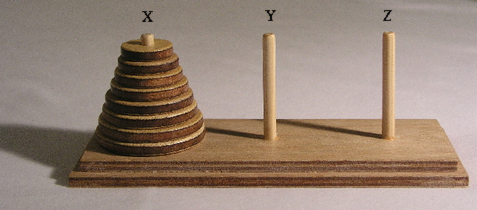
\includegraphics[width=180pt]{Tower-of-Hanoi.png}\\
\figcaption{Hanoi塔问题}\label{fig:hanoiTower}
\end{center}


现要求将X塔上的n个圆盘移动到Z上并仍按同样的顺序叠放,圆盘移动时必须遵循下列规则:
\begindot
\item 每次只能移动一个圆盘;
\item 圆盘可以插在X、Y和Z中的任一塔座上;
\item 任何时刻都不能将一个较大的圆盘压在较小的圆盘之上。
\myenddot

递归代码如下:
\begin{Codex}[label=hanoi.c]
/*
 * @brief 将塔座x上按直径有小到大且自上而下编号
 * 为1至n的n个圆盘按规则搬到塔座z上,y可用做辅助塔座.
 * @param[in] n 圆盘个数
 * @param[in] x 源塔座
 * @param[in] y 辅助塔座
 * @param[in] z 目标塔座
 * @return 无
 * @note 无
 * @remarks 无
 */
static void hanoi(int n, char x, char y, char z)
{
    if(n ==  1) {
        /* 移动操作move(x,n,z)可定义为(c是初始值为的全局
           变量,对搬动计数):
           printf("%i. Move disk %i from %c to %c\n",
                                        ++c, n, x, z);
        */
        move(1, x, z); /* 将编号为1的圆盘从x移动到z */
        return;
    } else {
        /* 将x上编号1至n-1的圆盘移到y,z作辅助塔*/
        hanoi(n-1, x, z, y); 
        move(n,x,z);  /* 将编号为n的圆盘从x移到z */
        /* 将y上编号至n-1的圆盘移到z,x作辅助塔*/
        hanoi(n-1, y, x, z); 
    }
}
\end{Codex}

\subsection{数制转换}
\begin{Codex}[label=convert_base.cpp]
 /*
  * @brief 数制转换,将一个整数转化为 d进制,d<=16.
  * @param[in] n 整数n
  * @param[in] d d进制
  * @return 无
  */
static void convert_base(int n, const int d)
{
	std::stack<int> s;
	int e;

	while(n != 0) {
		e = n % d;
		s.push(e);
		n /= d;
	}
	while(!s.empty()) {
		e = s.top();
		s.pop();
		printf("%x", e);
	}
	return;
}

#define MAX 64 // 栈的最大长度
static int stack[MAX];
static int top = -1;
 /*
  * @brief 数制转换,将一个整数转化为 d进制,d<=16,更优化的版本.
  *
  * 如果可以预估栈的最大空间,则用数组来模拟栈,这时常用的一个技巧。
  * 这里,栈的最大长度是多少?假设CPU是64位,最大的整数则是2^64,由于
  * 数制最小为2,在这个进制下,数的位数最长,这就是栈的最大长度,最长为64。
  *
  * @param[in] n 整数n
  * @param[in] d d进制
  * @return 无
  */
static void convert_base2(int n, const int d)
{
	int e;

	while(n != 0) {
		e = n % d;
		stack[++top] = e; // push
		n /= d;
	}
	while(top >= 0) {
		e = stack[top--]; // pop
		printf("%x", e);
	}
	return;
}
\end{Codex}

\section{队列} %%%%%%%%%%%%%%%%%%%%%%%%%%%%%%

\subsection{打印杨辉三角}

\begin{Codex}[label=yanghui_triangle.cpp]
#include <queue>
/**
 * @brief 打印杨辉三角系数.
 *
 * 分行打印二项式(a+b)^n展开式的系数。在输出上一行
 * 系数的同时,将其下一行的系数预先计算好,放入队列中。
 * 在各行系数之间插入一个0。
 *
 * @param[in] n (a+b)^n
 * @return 无
 */
void yanghui_triangle(const int n)
{
    int i = 1;
    std::queue<int> q;
    /* 预先放入第一行的1 */
    q.push(i);

    for(i = 0; i <= n; i++) {	 /* 逐行处理*/
        int j;
        int s = 0;
        q.push(s);      /* 在各行间插入一个0*/

        /* 处理第i行的i+2个系数(包括一个0)*/
        for(j = 0; j < i+2; j++) {
            int t;
            int tmp;
            t = q.front();  /*读取一个系数,放入t*/
            q.pop();
            tmp = s + t;      /* 计算下一行系数,并进队列*/
            q.push(tmp);
            s = t;            /* 打印一个系数,第i+2个是0*/
            if(j != i+1) {
                printf("%d ",s);    
            }
        }
        printf("\n"); 
    }
}
\end{Codex}

\chapter{树}

\section{二叉树的遍历} %%%%%%%%%%%%%%%%%%%%%%%%%%%%%%
\label{sec:binaryTreeTraversal}

在中序遍历中,一个节点的前驱,是其左子树的最右下角结点,后继,是其右子树的最左下角结点。

在后序遍历中,
\begindot
\item 若结点是根结点,则其后继为空;
\item 若结点是双亲的右子树,或是左子树但双亲无右子树,则其后继为双亲结点;
\item 若结点是双亲的左子树且双亲有右子树,则其后继为右子树按后序遍历的第一个结点
\myenddot


\begin{Codex}[label=binary_tree.cpp]
#include <stack>
#include <queue>

 /*
  *@struct
  *@brief 二叉树结点
  */
typedef struct binary_tree_node_t {
    binary_tree_node_t *lchild;   /* 左孩子*/
    binary_tree_node_t *rchild;   /* 右孩子*/
    void* data; /* 结点的数据*/
}binary_tree_node_t;

/** 
  * @brief 先序遍历,递归.
  * @param[in] root 根结点
  * @param[in] visit 访问数据元素的函数指针
  * @return 无
  */
void pre_order_r(const binary_tree_node_t *root, 
                 int (*visit)(void*)) {
    if(root != NULL) {
        (void)visit(root->data);
        pre_order_r(root->lchild, visit);
        pre_order_r(root->rchild, visit);
    }
}

/** 
  * @brief 中序遍历,递归.
  */
void in_order_r(const binary_tree_node_t *root, 
                int (*visit)(void*)) {
    if(root != NULL) {
        pre_order_r(root->lchild, visit);
        (void)visit(root->data);
        pre_order_r(root->rchild, visit);
    }
}

/** 
  * @brief 后序遍历,递归.
  */
void post_order_r(const binary_tree_node_t *root, 
                  int (*visit)(void*)) {
    if(root != NULL) {
        pre_order_r(root->lchild, visit);
        pre_order_r(root->rchild, visit);
        (void)visit(root->data);
    }
}

/** 
 * @brief 先序遍历,非递归.
 */
void pre_order(const binary_tree_node_t *root, 
               int (*visit)(void*)) {
    const binary_tree_node_t *p;
    std::stack<const binary_tree_node_t *> s;

    p = root;

    if(p != NULL) {
        s.push(p);
    }

    while(!s.empty()) {
        p = s.top();
        s.pop();
        visit(p->data);
        if(p->rchild != NULL) {
            s.push(p->rchild);
        }
        if(p->lchild != NULL) {
            s.push(p->lchild);
        }
    }
}

/** 
 * @brief 中序遍历,非递归.
 */
void in_order(const binary_tree_node_t *root, 
              int (*visit)(void*)) {
    const binary_tree_node_t *p;
    std::stack<const binary_tree_node_t *> s;

    p = root;

    while(!s.empty() || p!=NULL) {
        if(p != NULL) {
            s.push(p);
            p = p->lchild;
        } else {
            p = s.top();
            s.pop();
            visit(p->data);
            p = p->rchild;
        }
    }
}

/** 
 * @brief 后序遍历,非递归.
 */
void post_order(const binary_tree_node_t *root, 
                int (*visit)(void*)) {
    /* p,正在访问的结点,q,刚刚访问过的结点*/
    const binary_tree_node_t *p, *q;
    std::stack<const binary_tree_node_t *> s;

    p = root;

    do {
        while(p != NULL) { /* 往左下走*/
            s.push(p);
            p = p->lchild;
        }
        q = NULL;
        while(!s.empty()) {
            p = s.top();
            s.pop();
            /* 右孩子不存在或已被访问,访问之*/
            if(p->rchild == q) {
                visit(p->data);
                q = p; /* 保存刚访问过的结点*/
            } else {
                /* 当前结点不能访问,需第二次进栈*/
                s.push(p);
                /* 先处理右子树*/
                p = p->rchild;
                break;
            }
        }
    }while(!s.empty());
}

/** 
 * @brief 层次遍历,也即BFS.
 *
 * 跟先序遍历一模一样,唯一的不同是栈换成了队列
 */
void level_order(const binary_tree_node_t *root, 
                 int (*visit)(void*)) {
    const binary_tree_node_t *p;
    std::queue<const binary_tree_node_t *> q;

    p = root;

    if(p != NULL) {
        q.push(p);
    }

    while(!q.empty()) {
        p = q.front();
        q.pop();
        visit(p->data);
        if(p->lchild != NULL) { /*先左后右或先右后左无所谓*/
            q.push(p->lchild);
        }
        if(p->rchild != NULL) {
            q.push(p->rchild);
        }
    }
}
\end{Codex}

\section{线索二叉树} %%%%%%%%%%%%%%%%%%%%%%%%%%%%%%
二叉树中存在很多空指针,可以利用这些空指针,指向其前驱或者后继。这种利用起来的空指针称为线索,这种改进后的二叉树称为线索二叉树(threaded binary tree)。

一棵n个结点的二叉树含有n+1个空指针。这是因为,假设叶子节点数为$n_0$,度为1的节点数为$n_1$,度为2的节点数为$n_2$,每个叶子节点有2个空指针,每个度为1的节点有1个空指针,则空指针的总数为$2n_0+n_1$,又有$n_0=n_2+1$(留给读者证明),因此空指针总数为$2n_0+n_1=n_0+n_2+1+n_1=n_0+n_1+n_2+1=n+1$。

在二叉树线索化过程中,通常规定,若无左子树,令lchild指向前驱,若无右子树,令rchild指向后继。还需要增加两个标志域表示当前指针是不是线索,例如ltag=1,表示lchild指向的是前驱,ltag=0,表示lchild指向的是左孩子,rtag类似。

二叉树的线索化,实质上就是遍历一棵树,只是在遍历的过程中,检查当前节点的左右指针是否为空,若为空,将它们改为指向前驱或后继的线索。

以中序线索二叉树为例,指针pre表示前驱,succ表示后继,如图~\ref{fig:threadedBinaryTree}所示。

\begin{center}
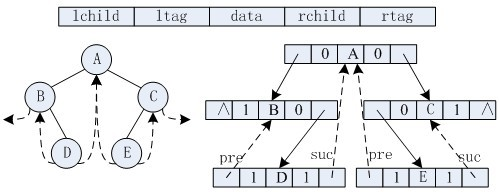
\includegraphics[width=300pt]{threaded-binary-tree.png} \\
\figcaption{中序线索二叉树}\label{fig:threadedBinaryTree}
\end{center}

在中序线索二叉树中,一个节点的前驱,是其左子树的最右下角结点,后继,是其右子树的最左下角结点。

中序线索二叉树的C语言实现如下。
\begin{Codex}[label=theaded_binary_tree.c]
/** @file threaded_binary_tree.c
  * @brief 线索二叉树.
  * @author soulmachine@gmail.com
  * @date 2013-06-16
  */
#include <stddef.h>    /* for NULL */
#include <stdio.h>

/* 结点数据的类型. */
typedef int elem_t;

 /**
  *@struct
  *@brief 线索二叉树结点.
  */
typedef struct tbt_node_t {
    int ltag; /** 1表示是线索,0表示是孩子 */
    int rtag; /** 1表示是线索,0表示是孩子 */
    struct tbt_node_t *lchild; /** 左孩子*/
    struct tbt_node_t *rchild; /** 右孩子*/
    elem_t data; /** 结点所存放的数据*/
}tbt_node_t;

/* 内部函数 */
static void in_thread(tbt_node_t *p, tbt_node_t **pre);
static tbt_node_t *first(tbt_node_t *p);
static tbt_node_t *next(const tbt_node_t *p);

 /**
  * @brief 建立中序线索二叉树.
  * @param[in] root 树根
  * @return 无
  */
void create_in_thread(tbt_node_t *root) {
    /* 前驱结点指针*/
	tbt_node_t *pre=NULL;
    if(root != NULL) { /* 非空二叉树,线索化*/
        /* 中序遍历线索化二叉树*/
        in_thread(root, &pre);
        /* 处理中序最后一个结点*/
        pre->rchild = NULL;
        pre->rtag = 1;
    }
}


/**
  * @brief 在中序线索二叉树上执行中序遍历.
  * @param[in] root 树根
  * @param[in] visit 访问结点的数据的函数
  * @return 无
  */
void in_order(tbt_node_t *root, int(*visit)(elem_t*)) {
	tbt_node_t *p;
    for(p = first(root); p != NULL; p = next(p)) {
        (void)visit(&(p->data));
    }
}


 /*
  * @brief 中序线索化二叉树的主过程.
  * @param[in] p 当前要处理的结点
  * @param[inout] pre 当前结点的前驱结点
  * @return 无
  */
static void in_thread(tbt_node_t *p, tbt_node_t **pre) {
    if(p != NULL) {
        in_thread(p->lchild, pre); /* 线索化左子树 */
        if(p->lchild == NULL) {  /* 左子树为空,建立前驱 */
            p->lchild = *pre;
            p->ltag = 1;
        }
        /* 建立前驱结点的后继线索 */
        if((*pre) != NULL &&
            (*pre)->rchild == NULL) {
            (*pre)->rchild = p;
            (*pre)->rtag = 1;
        }
        *pre = p; /* 更新前驱 */
        in_thread(p->rchild, pre); /* 线索化右子树 */
    }
}

 /*
  * @brief 寻找线索二叉树的中序下的第一个结点.
  * @param[in] p 线索二叉树中的任意一个结点
  * @return 此线索二叉树的第一个结点
  */
static tbt_node_t *first(tbt_node_t *p) {
    if(p == NULL)  return NULL;

    while(p->ltag == 0) {
        p = p->lchild;  /* 最左下结点,不一定是叶结点*/
    }
    return p;
}

 /*
  * @brief 求中序线索二叉树中某结点的后继.
  * @param[in] p 某结点
  * @return p的后继
  */
static tbt_node_t *next(const tbt_node_t *p) {
    if(p->rtag == 0) {
        return first(p->rchild);
    } else {
        return p->rchild;
    }
}
\end{Codex}

中序线索二叉树最简单,在中序线索的基础上稍加修改就可以实现先序,后续就要再费点心思了。


\section{Morris Traversal} %%%%%%%%%%%%%%%%%%%%%%%%%%%%%%
通过前面第\S \ref{sec:binaryTreeTraversal}节,我们知道,实现二叉树的前序(preorder)、中序(inorder)、后序(postorder)遍历有两个常用的方法,一是递归(recursive),二是栈(stack+iterative)。这两种方法都是O(n)的空间复杂度。

而Morris Traversal只需要O(1)的空间复杂度。这种算法跟线索二叉树很像,不过Morris Traversal一边建线索,一边访问数据,访问完后销毁线索,保持二叉树不变。

\subsection{Morris中序遍历}
Morris中序遍历的步骤如下:
\begin{enumerate}
\item 初始化当前节点cur为root节点
\item 如果cur没有左孩子,则输出当前节点并将其右孩子作为当前节点,即cur = cur->rchild。
\item 如果cur有左孩子,则寻找cur的前驱,即cur的左子树的最右下角结点。\\
   a) 如果前驱节点的右孩子为空,将它的右孩子指向当前节点,当前节点更新为当前节点的左孩子。\\
   b) 如果前驱节点的右孩子为当前节点,将它的右孩子重新设为空(恢复树的形状),输出当前节点,当前节点更新为当前节点的右孩子。
\item 重复2、3步骤,直到cur为空。
\end{enumerate}
如图~\ref{fig:inorderMorris}所示,cur表示当前节点,深色节点表示该节点已输出。

\begin{center}
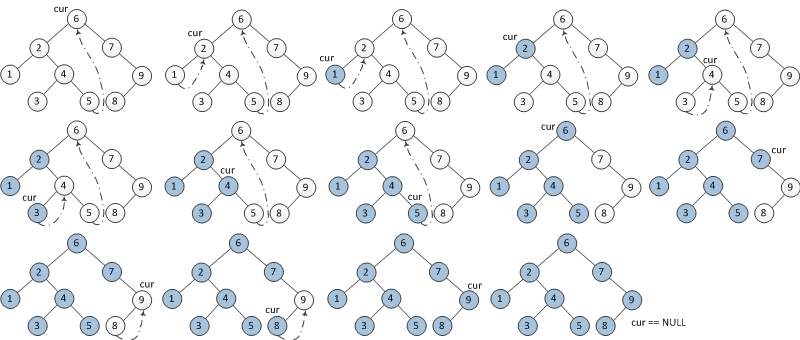
\includegraphics[width=360pt]{inorder-morris-traversal.png} \\
\figcaption{Morris中序遍历}\label{fig:inorderMorris}
\end{center}

C语言实现见第\S\ref{sec:morrisTraversalImpl}节。

\subsubsection{相关的题目}
\begindot
\item Leet Code - Binary Tree Inorder Traversal, \myurl{http://leetcode.com/onlinejudge\#question_94}
\myenddot


\subsection{Morris先序遍历}
Morris先序遍历的步骤如下:
\begin{enumerate}
\item 初始化当前节点cur为root节点
\item 如果cur没有左孩子,则输出当前节点并将其右孩子作为当前节点,即cur = cur->rchild。
\item 如果cur有左孩子,则寻找cur的前驱,即cur的左子树的最右下角结点。\\
   a) 如果前驱节点的右孩子为空,将它的右孩子指向当前节点,\textbf{输出当前节点(在这里输出,这是与中序遍历唯一的不同点)}当前节点更新为当前节点的左孩子。\\
   b) 如果前驱节点的右孩子为当前节点,将它的右孩子重新设为空(恢复树的形状),\sout{输出当前节点,}当前节点更新为当前节点的右孩子。
\item 重复2、3步骤,直到cur为空。
\end{enumerate}
如图~\ref{fig:preorderMorris}所示。

\begin{center}
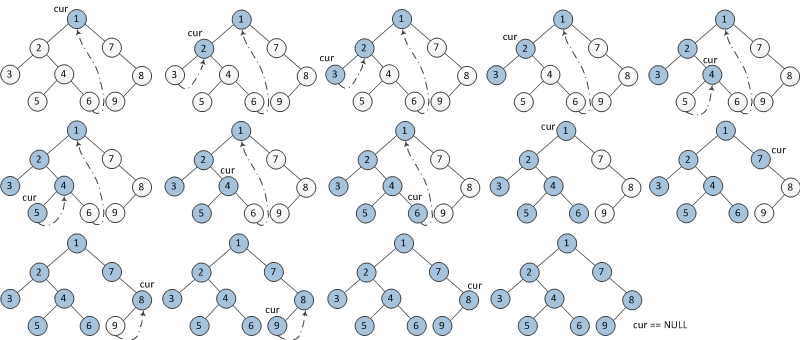
\includegraphics[width=360pt]{preorder-morris-traversal.png} \\
\figcaption{Morris先序遍历}\label{fig:preorderMorris}
\end{center}

C语言实现见第\S\ref{sec:morrisTraversalImpl}节。


\subsection{Morris后序遍历}
Morris后续遍历稍微复杂,需要建立一个临时节点dump,令其左孩子是root,并且还需要一个子过程,就是倒序输出某两个节点之间路径上的所有节点。

Morris后序遍历的步骤如下:
\begin{enumerate}
\item 初始化当前节点cur为root节点
\item 如果cur没有左孩子,则\sout{输出当前节点并}将其右孩子作为当前节点,即cur = cur->rchild。
\item 如果cur有左孩子,则寻找cur的前驱,即cur的左子树的最右下角结点。\\
   a) 如果前驱节点的右孩子为空,将它的右孩子指向当前节点,当前节点更新为当前节点的左孩子。\\
   b) 如果前驱节点的右孩子为当前节点,将它的右孩子重新设为空(恢复树的形状),\sout{输出当前节点,}\textbf{倒序输出从当前节点的左孩子到该前驱节点这条路径上的所有节点。}当前节点更新为当前节点的右孩子。
\item 重复2、3步骤,直到cur为空。
\end{enumerate}
如图~\ref{fig:postorderMorris}所示。

\begin{center}
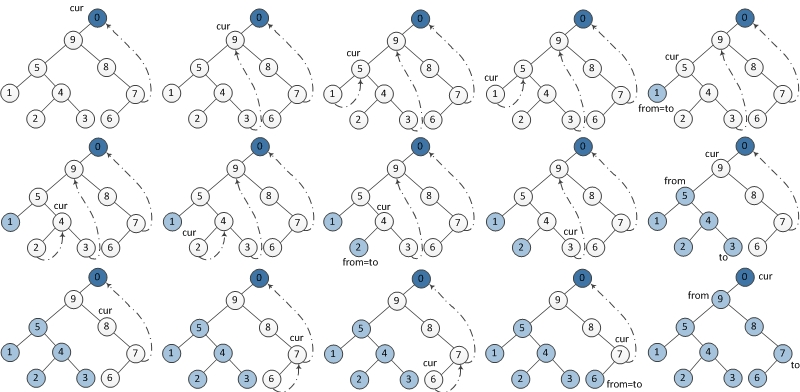
\includegraphics[width=360pt]{postorder-morris-traversal.png} \\
\figcaption{Morris后序遍历}\label{fig:postorderMorris}
\end{center}

C语言实现见第\S\ref{sec:morrisTraversalImpl}节。


\subsection{C语言实现}
\label{sec:morrisTraversalImpl}
\begin{Codex}[label=morris_traversal.cpp]
/** @file morris_traversal.c
 * @brief Morris遍历算法.
 * @author soulmachine@gmail.com
 * @date 2013-06-16
 */
#include<stdio.h>
#include<stdlib.h>

/* 结点数据的类型. */
typedef int elem_t;

/**
 *@struct
 *@brief 二叉树结点.
 */
typedef struct bt_node_t {
    elem_t data; /* 节点的数据 */
    struct bt_node_t *lchild; /* 左孩子 */
    struct bt_node_t *rchild; /* 右孩子 */
} bt_node_t;

/**
 * @brief 中序遍历,Morris算法.
 * @param[in] root 根节点
 * @param[in] visit 访问函数
 * @return 无
 */
void in_order_morris(bt_node_t *root, int(*visit)(elem_t*)) {
    bt_node_t *cur, *pre;

    cur = root;
    while (cur != NULL ) {
        if (cur->lchild == NULL ) {
            visit(cur->data);
            cur = cur->rchild;
        } else {
            /* 查找前驱 */
            pre = cur->lchild;
            while (pre->rchild != NULL && pre->rchild != cur)
                pre = pre->rchild;

            if (pre->rchild == NULL ) {    /* 还没线索化,则建立线索 */
                pre->rchild = cur;
                cur = cur->lchild;
            } else {    /* 已经线索化,则访问节点,并删除线索  */
                visit(cur->data);
                pre->rchild = NULL;
                cur = cur->rchild;
            }
        }
    }
}

/**
 * @brief 先序遍历,Morris算法.
 * @param[in] root 根节点
 * @param[in] visit 访问函数
 * @return 无
 */
void pre_order_morris(bt_node_t *root, int (*visit)(elem_t*)) {
    bt_node_t *cur = root, *pre = NULL;
    while (cur != NULL ) {
        if (cur->lchild == NULL ) {
            visit(cur->data);
            cur = cur->rchild;
        } else {
            pre = cur->lchild;
            while (pre->rchild != NULL && pre->rchild != cur)
                pre = pre->rchild;

            if (pre->rchild == NULL ) {
                visit(cur->data);  // 仅这一行与中序不同
                pre->rchild = cur;
                cur = cur->lchild;
            } else {
                pre->rchild = NULL;
                cur = cur->rchild;
            }
        }
    }
}

static void reverse(bt_node_t *from, bt_node_t *to);
static void visit_reverse(bt_node_t* from, bt_node_t *to, int (*visit)(elem_t*));
/**
 * @brief 后序遍历,Morris算法.
 * @param[in] root 根节点
 * @param[in] visit 访问函数
 * @return 无
 */
void post_order_morris(bt_node_t *root, int (*visit)(elem_t*)) {
    bt_node_t dump = { 0, NULL, NULL };
    dump.lchild = root;
    bt_node_t *cur = &dump, *pre = NULL;
    while (cur != NULL ) {
        if (cur->lchild == NULL ) {
            cur = cur->rchild;
        } else {
            pre = cur->lchild;
            while (pre->rchild != NULL && pre->rchild != cur)
                pre = pre->rchild;

            if (pre->rchild == NULL ) {
                pre->rchild = cur;
                cur = cur->lchild;
            } else {
                visit_reverse(cur->lchild, pre, visit);  // call print
                pre->rchild = NULL;
                cur = cur->rchild;
            }
        }
    }
}

/*
 * @brief 逆转路径.
 * @param[in] from from
 * @param[to] to to
 * @return 无
 */
static void reverse(bt_node_t *from, bt_node_t *to) {
    if (from == to) return;
    bt_node_t *x = from, *y = from->rchild, *z;
    while (x != to) {
        z = y->rchild;
        y->rchild = x;
        x = y;
        y = z;
    }
}

/*
 * @brief  访问逆转后的路径上的所有结点.
 * @param[in] from from
 * @param[to] to to
 * @return 无
 */
static void visit_reverse(bt_node_t* from, bt_node_t *to, int (*visit)(elem_t*)) {
    reverse(from, to);

    bt_node_t *p = to;
    while (1) {
        visit(p->data);
        if (p == from)
            break;
        p = p->rchild;
    }

    reverse(to, from);
}

/*
 * @brief 分配一个新节点.
 * @param[in] data 新节点的数据
 * @return 新节点
 */
bt_node_t* new_node(int data) {
    bt_node_t* node = (bt_node_t*) malloc(sizeof(bt_node_t));
    node->data = data;
    node->lchild = NULL;
    node->rchild = NULL;

    return (node);
}

static int print(const elem_t *data) {
    printf(" %d ", data);
    return 0;
}

/* test */
int main() {
    /* 构造的二叉树如下
       1
     /   \
    2      3
  /  \
4     5
     */
    bt_node_t *root = new_node(1);
    root->lchild = new_node(2);
    root->rchild = new_node(3);
    root->lchild->lchild = new_node(4);
    root->lchild->rchild = new_node(5);

    in_order_morris(root, print);
    printf("\n");
    pre_order_morris(root, print);
    printf("\n");
    post_order_morris(root, print);

    return 0;
}
\end{Codex}


\section{重建二叉树} %%%%%%%%%%%%%%%%%%%%%%%%%%%%%%
\begin{Codex}[label=binary_tree.cpp]
/** 
 * @brief 给定前序遍历和中序遍历,输出后序遍历.
 *
 * @param[in] n 序列的长度
 * @param[in] pre 前序遍历的序列
 * @param[in] in 中序遍历的序列
 * @param[out] post 后续遍历的序列
 * @return 无
 */
void build(const int n, const char * pre, const char *in, char *post) {
	if(n <= 0) return;
	int p = strchr(in, pre[0]) - in;
	build(p, pre + 1, in, post);
	build(n - p - 1, pre + p + 1, in + p + 1, post + p);
	post[n - 1] = pre[0];
}

// 测试
// BCAD CBAD,输出 CDAB
// DBACEGF ABCDEFG,输出 ACBFGED
int build_test() {
    const int MAX = 64;
    char pre[MAX] = {0};
    char in[MAX] = {0};
    char post[MAX] = {0};
    scanf("%s%s", pre, in);
    
    const int n = strlen(pre);
    build(n, pre, in, post);
    printf("%s\n", post);
}
\end{Codex}


\section{堆} %%%%%%%%%%%%%%%%%%%%%%%%%%%%%%

\subsection{堆的C语言实现}
C++可以直接使用\fn{std::priority_queue}。

\begin{Codex}[label=heap.c]
/** @file heap.c
 * @brief 堆,默认为小根堆,即堆顶为最小.
 * @author soulmachine@gmail.com
 * @date 2010-8-1
 * @version 1.0
 */
#include <stdlib.h>  /* for malloc() */
#include <string.h>  /* for memcpy() */

typedef int heap_elem_t; // 元素的类型

/**
 * @struct
 * @brief 堆的结构体
 */
typedef struct heap_t {
    int     size;   /** 实际元素个数 */
    int     capacity; /** 容量,以元素为单位 */
    heap_elem_t  *elems;   /** 堆的数组 */
    int (*cmp)(const heap_elem_t*, const heap_elem_t*);   /** 元素的比较函数 */
}heap_t;


/** 基本类型(如int, long, float, double)的比较函数 */
int cmp_int(const heap_elem_t *x, const heap_elem_t *y) {
    const int sub = *x - *y;
    if(sub > 0) {
        return 1;
    } else if(sub < 0) {
        return -1;
    } else {
        return 0;
    }
}

/** 
 * @brief 堆的初始化.
 * @param[out] h 堆对象的指针
 * @param[out] capacity 初始容量
 * @param[in] cmp cmp 比较函数,小于返回-1,等于返回0
 * 大于返回1,反过来则是大根堆
 * @return 成功返回0,失败返回错误码
 */
int heap_init(heap_t *h, const int capacity, 
              int (*cmp)(const heap_elem_t*, const heap_elem_t*)) {
    h->size = 0;
    h->capacity = capacity;
    h->elems = (heap_elem_t*)malloc(capacity * sizeof(heap_elem_t));
    h->cmp = cmp;
    
    return 0;
}

/** 
 * @brief 释放堆.
 * @param[inout] h 堆对象的指针
 * @return 成功返回0,失败返回错误码
 */
int heap_uninit(heap_t *h) {
    h->size = 0;
    h->capacity = 0;
    free(h->elems);
    h->elems = NULL;
    h->cmp = NULL;

    return 0;
}


/** 
 * @brief 判断堆是否为空.
 * @param[in] h 堆对象的指针
 * @return 是空,返回 1,否则返回 0
 */
int heap_empty(const heap_t *h) {
    return h->size == 0;
}

/** 
 * @brief 获取元素个数.
 * @param[in] s 堆对象的指针
 * @return 元素个数
 */
int heap_size(const heap_t *h) {
    return h->size;
}

/*
 * @brief 小根堆的自上向下筛选算法.
 * @param[in] h 堆对象的指针
 * @param[in] start 开始结点
 * @return 无
 */
void heap_sift_down(const heap_t *h, const int start) {
    int i = start;
    int j;
    const heap_elem_t tmp = h->elems[start];
       
    for(j = 2 * i + 1; j < h->size; j = 2 * j + 1) {
        if(j < (h->size - 1) && 
            // h->elems[j] > h->elems[j + 1]
            h->cmp(&(h->elems[j]), &(h->elems[j + 1])) > 0) {
                j++; /* j 指向两子女中小者*/
        }
        // tmp <= h->data[j]
        if(h->cmp(&tmp, &(h->elems[j])) <= 0) {
            break;
        } else {
            h->elems[i] = h->elems[j];
            i = j;
        }
    }
    h->elems[i] = tmp;
}
 
/* 
 * @brief 小根堆的自下向上筛选算法.
 * @param[in] h 堆对象的指针
 * @param[in] start 开始结点
 * @return 无
 */
void heap_sift_up(const heap_t *h, const int start) {
    int j = start;
    int i= (j - 1) / 2;
    const heap_elem_t tmp = h->elems[start];
 
    while(j > 0) {
        // h->data[i] <= tmp
        if(h->cmp(&(h->elems[i]), &tmp) <= 0) {
            break;
        } else {
            h->elems[j] = h->elems[i];
            j = i;
            i = (i - 1) / 2;
        }
    }
    h->elems[j] = tmp;
}

/** 
 * @brief 添加一个元素.
 * @param[in] h 堆对象的指针
 * @param[in] x 要添加的元素
 * @return 无
 */
void heap_push(heap_t *h, const heap_elem_t x) {
    if(h->size == h->capacity) { /*已满,重新分配内存*/
        heap_elem_t* tmp = 
            (heap_elem_t*)realloc(h->elems, h->capacity * 2 * sizeof(heap_elem_t));
        h->elems = tmp;
        h->capacity *= 2;
    }
 
    h->elems[h->size] = x;
    h->size++;

    heap_sift_up(h, h->size - 1);
}

/** 
 * @brief 弹出堆顶元素.
 * @param[in] h 堆对象的指针
 * @return 无
 */
void heap_pop(heap_t *h) {
    h->elems[0] = h->elems[h->size - 1];
    h->size --;
    heap_sift_down(h, 0);
}

/** 
 * @brief 获取堆顶元素.
 * @param[in] h 堆对象的指针
 * @return 堆顶元素
 */
heap_elem_t heap_top(const heap_t *h) {
    return h->elems[0];
}
\end{Codex}
\chapter{查找}

\section{折半查找} %%%%%%%%%%%%%%%%%%%%%%%%%%%%%%

\begin{Codex}[label=binary_search.c]
/** 数组元素的类型 */
typedef int elem_t;
/**
  * @brief 有序顺序表的折半查找算法.
  *
  * @param[in] a 存放数据元素的数组,已排好序
  * @param[in] n 数组的元素个数
  * @param[in] x 要查找的元素
  * @return 查找成功则返回元素所在下标,否则返回-1
  */
int binary_search(const elem_t a[], const int n, const elem_t x) {
    int left = 0, right = n -1, mid;
    while(left <= right) {
        mid = left + (right - left) / 2;
        if(x > a[mid]) {
            left = mid + 1;
        } else if(x < a[mid]) {
            right = mid - 1;
        } else {
            return mid;
        }
    }
    return -1;
}
\end{Codex}


\section{哈希表} %%%%%%%%%%%%%%%%%%%%%%%%%%%%%%


\subsection{原理和实现}
\label{sec:hash-set}
哈希表处理冲突有两种方式,开地址法(Open Addressing)和闭地址法(Closed Addressing)。

闭地址法也即拉链法(Chaining),每个哈希地址里不再是一个元素,而是链表的首地址。

开地址法有很多方案,有线性探测法(Linear Probing)、二次探测法(Quodratic Probing)和双散列法(Double Hashing)等。

下面是拉链法的C语言实现。

\subsubsection{代码}
\begin{Codex}[label=hash_set.c]
#include <stdio.h>
#include <string.h>
#include <stdlib.h>

#ifndef __cplusplus
typedef char bool;
#define false 0
#define true 1
#endif

/** 每个元素所带的数据 */
typedef int hash_set_elem_t;

/** 哈希表容量,一定要大于元素最大个数  */
#define HASH_SET_CAPACITY  100001
/** 哈希表取模的质数,也即哈希桶的个数,小于 HASH_SET_CAPACITY. */
#define PRIME  99997

/** 哈希集合. */
typedef struct hash_set_t {
    int head[PRIME];  /** 首节点下标 */

    struct {
        hash_set_elem_t elem;
        int next;
    } node[HASH_SET_CAPACITY];  /** 静态链表 */

    int size; /** 实际元素个数 */

    int (*hash)(const hash_set_elem_t *elem); /** 元素的哈希函数 */
    bool (*cmp)(const hash_set_elem_t *elem1,
            const hash_set_elem_t *elem2);  /** 元素的比较函数 */
} hash_set_t;

/** 创建一个哈希集合. */
hash_set_t* hash_set_create(int (*hash)(const hash_set_elem_t *elem),
        bool (*cmp)(const hash_set_elem_t *elem1,
                const hash_set_elem_t *elem2)) {
    hash_set_t *result = (hash_set_t*)malloc(sizeof(hash_set_t));
    memset(result->head, -1, sizeof(result->head));
    memset(result->node, -1, sizeof(result->node));
    result->size = 0;
    result->hash = hash;
    result->cmp = cmp;
    return result;
}

/** 销毁哈希集合. */
void hash_set_destroy(hash_set_t *set) {
    free(set);
    set = NULL;
}

/** 查找某个元素是否存在. */
bool hash_set_find(const hash_set_t *set, const hash_set_elem_t *elem) {
    int i;
    int hash = set->hash(elem);

    for (i = set->head[hash]; i != -1; i = set->node[i].next) {
        if (set->cmp(elem, &(set->node[i].elem))) {
            return true;
        }
    }
    return false;
}

/** 添加一个元素,如果已存在则添加失败. */
bool hash_set_add(hash_set_t *set, const hash_set_elem_t *elem) {
    int i;
    int hash = set->hash(elem);

    for (i = set->head[hash]; i != -1; i = set->node[i].next) {
        if (set->cmp(elem, &(set->node[i].elem))) {
            return false; /* 已经存在 */
        }
    }
    /* 不存在,则插入在首节点之前 */
    set->node[set->size].next = set->head[hash];
    set->node[set->size].elem = *elem;
    set->head[hash] = set->size++;
    return true;
}
\end{Codex}


\subsection{Babelfish}


\subsubsection{描述}
You have just moved from Waterloo to a big city. The people here speak an incomprehensible dialect of a foreign language. Fortunately, you have a dictionary to help you understand them.


\subsubsection{输入}
Input consists of up to 100,000 dictionary entries, followed by a blank line, followed by a message of up to 100,000 words. Each dictionary entry is a line containing an English word, followed by a space and a foreign language word. No foreign word appears more than once in the dictionary. The message is a sequence of words in the foreign language, one word on each line. Each word in the input is a sequence of at most 10 lowercase letters.


\subsubsection{输出}
Output is the message translated to English, one word per line. Foreign words not in the dictionary should be translated as "eh".


\subsubsection{样例输入}
\begin{Code}
dog ogday
cat atcay
pig igpay
froot ootfray
loops oopslay

atcay
ittenkay
oopslay
\end{Code}


\subsubsection{样例输出}
\begin{Code}
cat
eh
loops
\end{Code}


\subsubsection{分析}
最简单的方法是,把输入的单词对,存放在一个数组,排好序,查找的时候每次进行二分查找。

更快的方法是,用HashMap。C++有\fn{std::map},C++ 11以后有\fn{std::unordered_map},比\fn{std::map}快。也可以自己实现哈希表。


\subsubsection{代码}
使用 \fn{std::map} 。

\begin{Codex}[label=babelfish_map.cpp]
/* POJ 2503 Babelfish , http://poj.org/problem?id=2503 */
#include <cstdio>
#include <map>
#include <string>
#include <cstring>

using namespace std;

/** 字符串最大长度 */
const int MAX_WORD_LEN = 10;

int main() {
    char line[MAX_WORD_LEN * 2 + 1];
    char s1[MAX_WORD_LEN + 1], s2[MAX_WORD_LEN + 1];
    map<string, string> dict;

    while (gets(line) && line[0] != 0) {
        sscanf(line, "%s %s", s1, s2);
        dict[s2] = s1;
    }

    while (gets(line)) {
        if (dict[line].length() == 0) puts("eh");
        else printf("%s\n", dict[line].c_str());
    }
    return 0;
}
\end{Codex}


自己实现哈希表。

\begin{Codex}[label=babelfish.c]
/* POJ 2503 Babelfish , http://poj.org/problem?id=2503 */
/** 单词最大长度. */
#define MAX_WORD_LEN   11

/** 每个元素所带的数据 */
typedef struct hash_set_elem_t {
    char english[MAX_WORD_LEN];
    char foreign[MAX_WORD_LEN];
} hash_set_elem_t;

/** 哈希表容量,一定要大于元素最大个数  */
#define HASH_SET_CAPACITY  100001
/** 哈希表取模的质数,也即哈希桶的个数,小于 HASH_SET_CAPACITY. */
#define PRIME  99997

/* 等价于复制粘贴,这里为了节约篇幅,使用include,在OJ上提交时请用复制粘贴 */
#include "hash_set.c"  /* 见“查找->哈希表”这节 */

/* 与hash_set_find() 略有不同,用类似于HashMap的方式 */
bool hash_set_get(const hash_set_t *set, hash_set_elem_t *elem) {
    int i;
    int hash = set->hash(elem);

    for (i = set->head[hash]; i != -1; i = set->node[i].next) {
        if (set->cmp(elem, &(set->node[i].elem))) {
            // 返回对应 english, foreigh 作为key, english作为value
            strncpy(elem->english, set->node[i].elem.english, MAX_WORD_LEN-1);
            return true;
        }
    }
    return false;
}

int elem_hash(const hash_set_elem_t *elem) {
    const char *str = elem->foreign;
    unsigned int r = 0;
    int len = strlen(str);
    int i;

    for (i = 0; i < len; i++) {
        r = (r * 31 + str[i]) % PRIME;
    }
    return r % PRIME;
}

bool elem_cmp(const hash_set_elem_t *elem1, const hash_set_elem_t *elem2) {
    return strcmp(elem1->foreign, elem2->foreign) == 0;
}

int main() {
    char line[MAX_WORD_LEN * 2];
    hash_set_t *set = hash_set_create(elem_hash, elem_cmp);
    hash_set_elem_t e;

    while (gets(line) && line[0] != 0) {
        sscanf(line, "%s %s", e.english, e.foreign);
        hash_set_add(set, &e);
    }
    while (gets(e.foreign)) {
        if (hash_set_get(set, &e)) printf("%s\n", e.english);
        else printf("eh\n");
    }
    hash_set_destroy(set);
    return 0;
}
\end{Codex}


\subsubsection{相关的题目}
与本题相同的题目:
\begindot
\item POJ 2503 Babelfish, \myurl{http://poj.org/problem?id=2503}
\myenddot

与本题相似的题目:
\begindot
\item  无
\myenddot

\chapter{排序}

\section{快速排序} %%%%%%%%%%%%%%%%%%%%%%%%%%%%%%

\begin{Codex}[label=quick_sort.c]
/** 数组元素的类型 */
typedef int elem_t;
 /*
  * @brief 一趟划分.
  * @param[inout] a 待排序元素序列
  * @param[in] start 开始位置
  * @param[in] end 结束位置,最后一个元素后一个位置
  * @return 基准元素的新位置
  */
static int partition(elem_t a[], const int start, const int end)
{
    int i = start;
    int j = end - 1;
    const elem_t pivot = a[i];

    while(i < j) {
        while(i < j && a[j] >= pivot) j--;
        a[i] = a[j];
        while(i < j && a[i] <= pivot) i++;
        a[j] = a[i];
    }
    a[i] = pivot;
    return i;
}

/**
  * @brief 快速排序.
  * @param[inout] a 待排序元素序列
  * @param[in] start 开始位置
  * @param[in] end 结束位置,最后一个元素后一个位置
  * @return 无
  */
void quick_sort(elem_t a[], const int start, const int end)
{
    if(start < end - 1) { /* 至少两个元素*/
        const int pivot_pos = partition(a, start, end);
        quick_sort(a, start, pivot_pos);
        quick_sort(a, pivot_pos + 1, end);
    }
}
\end{Codex}
\chapter{暴力枚举法}

\section{算法思想} %%%%%%%%%%%%%%%%%%%%%%%%%%%%%%
生成--测试法。

\section{简单枚举} %%%%%%%%%%%%%%%%%%%%%%%%%%%%%%

\subsection{分数拆分}
输入正整数$k$,找到所有的正整数 $x \geq y$,使得 $\dfrac{1}{k}=\dfrac{1}{x}+\dfrac{1}{y}$。

\textbf{样例输入}\\
2 \\
12 \\

\textbf{样例输出} \\
2 \\
1/2=1/6+1/3 \\
1/2=1/4+1/4 \\
8
1/12=1/156+1/13 \\
1/12=1/84+1/14 \\
1/12=1/60+1/15 \\
1/12=1/48+1/16 \\
1/12=1/36+1/18 \\
1/12=1/30+1/20 \\
1/12=1/28+1/21 \\
1/12=1/24+1/24 \\

\subsubsection{分析}
既然说找出所有的$x,y$,枚举对象自然就是他们了。可问题在于:枚举范围如何?
从$\dfrac{1}{12}=\dfrac{1}{156}+\dfrac{1}{13}$,可以看出,$x$可以比$y$大很多。
难道要无休止地枚举下去?当然不是。由于$x \geq y$,
有$\dfrac{1}{x} \leq \dfrac{1}{y}$,因此 $\dfrac{1}{k}-\dfrac{1}{y} \leq \dfrac{1}{y}$,
即$y \leq 2k$。这样,只需要在$2k$范围之类枚举$y$,然后根据$y$算出$x$即可。

\section{枚举排列} %%%%%%%%%%%%%%%%%%%%%%%%%%%%%%

\subsection{生成1~n的排列}

\subsection{生成可重复集合的排列}

\subsection{下一个排列}

\section{子集生成} %%%%%%%%%%%%%%%%%%%%%%%%%%%%%%

\subsection{增量构造法}

\subsection{位向量法}

\subsection{二进制法}

\chapter{广度优先搜索}
当题目看不出任何规律,既不能用分治,贪心,也不能用动规时,这时候万能方法——搜索,
就派上用场了。搜索分为广搜和深搜,广搜里面又有普通广搜,双向广搜,A*搜索等。
深搜里面又有普通深搜,回溯法等。

广搜和深搜非常类似(除了在扩展节点这部分不一样),二者有相同的框架,如何表示状态?
如何扩展状态?如何判重?尤其是判重,解决了这个问题,基本上整个问题就解决了。


\section{算法框架} %%%%%%%%%%%%%%%%%%%%%%%%%%%%%%
思考的步骤:
\begin{enumerate}
\item 如何表示状态?即一个状态需要存储哪些些必要的数据,就可以完整表示该状态?这一步不考虑是求长度还是求路径的问题,纯粹考虑状态本身的数据。
\item 是求最短路径长度,还是最短路径(或动作序列)?如果是求长度,则状态里面要存路径长度;如果是求路径或动作序列,则要用一棵树存储宽搜过程中的路径。
    \begin{enumerate}
    \item 如果是求长度,则状态里面要存路径长度
    \end{enumerate}
\item 是求最短路径长度,还是最短路径(或动作序列)?如果是求路径或动作序列
    \begin{enumerate}
    \item 要用一棵树存储宽搜过程中的路径
    \item 是否可以预估状态个数的上限?能够预估状态总数,则开一个大数组,用树的双亲表示法;如果不能预估状态总数,则要使用一棵通用的树(自己实现或用标准库)。这一步也是第4步的必要不充分条件。
   \end{enumerate}
\item 关于判重,状态是否存在完美哈希方案?即将状态一一映射到整数,互相之间不会冲突。
    \begin{enumerate}
    \item 如果不存在,则需要使用通用的哈希表(自己实现或用标准库,例如\fn{std::unordered_set})来判重;自己实现哈希表的话,如果能够预估状态个数的上限,则可以开两个数组,head和next,表示哈希表,参考第 \S \ref{subsec:eightDigits}节方案2。
    \item 如果存在,则可以开一个大布尔数组,作为哈希表来判重,且此时可以精确计算出状态总数,而不仅仅是预估上限。
    \end{enumerate}
\end{enumerate}

\begin{Codex}[label=bfs_template.c]
#include <stdio.h>
#include <string.h>

/***** 输入数据,用全局变量存放 *****/
...
/*
例如
int m = MAXN, n = MAXN;  // 迷宫的行数,列数
// 迷宫,0表示空地,1表示障碍物
int map[MAXN][MAXN];  // 迷宫,0表示空地,1表示障碍物
 */

/***** 一些常量 *****/
...
/* 例如
// 四个方向
const char name[4] = { 'U', 'R', 'D', 'L' };
const int dx[4] = { -1, 0, 1, 0 }; // 行
const int dy[4] = { 0, 1, 0, -1 }; // 列
*/

#ifndef __cplusplus
typedef char bool;
#define false 0
#define true 1
#endif

/**
 * @strut 状态
 */
typedef struct state_t {
    ... data1;  /** 状态的数据,可以有多个字段. */
    ... data2;  /** 状态的数据,可以有多个字段. */
    int action; /** 由父状态移动到本状态的动作 */
    int index;  /** 本状态在path[]中的下标,求路径或动作序列时需要。
                    如果存在完美哈希,则不需要本字段(此时将
                   状态的哈希值作为下标,而哈希值可以直接计算出) */
    int father; /** 父状态在path[]中的下标,,求路径或动作序列时需要 */
    int count;  /** 所花费的步骤数(也即路径长度-1),求路径长度时需要 */
} state_t;

/********** 如果题目要求输出路径或动作序列,则需要下面的变量和函数 ***********/

#define STATE_MAX ...  /* 状态总数 */
/**
 * 记录动作序列,树的双亲表示法.
 * 如果不能预估状态个数的上限,则不能用数组,要用通用树
 * 一般此时会有完美哈希方案,开一个大数组存储每个状态的动作,下标就是状态的哈希值
 * 其实一般用不了这么大的数组,广搜很很快就会结束
 */
state_t path[STATE_MAX];
int path_index = 0;  /** 每出现一个新状态,就增1,将状态存到该位置 */

/**
 * @brief 打印动作序列.
 * 如果有完美哈希方案,状态的哈希值就是下标。
 * 起点状态没有父亲和动作为-1,因为它没有父状态,也就没有所谓的从父节点到它的动作。
 * @param[in] end 终点状态的下标
 * @return 父状态
 */
void print_action(const int end) {
    if (path[end].father == -1) return;

    print_action(path[end].father);
    putchar(name[path[end].action]);
}

/**
 * @brief 打印坐标序列.
 * 如果有完美哈希方案,状态的哈希值就是下标。
 * 起点状态没有父亲和动作为-1,因为它没有父状态,也就没有所谓的从父节点到它的动作。
 * @param[in] end 终点状态的哈希值
 * @return 父状态
 */
void print_path(const int end) {
    if (path[end].father == -1) {
        printf("(%d, %d)\n", end / n, end % n);
        return;
    }
    print_path(path[end].father);
    printf("(%d, %d)\n", end / n, end % n);
}

/********** 如果题目要求输出路径或动作序列,则需要上面的变量和函数 ***********/

/** 计算状态的哈希值,如果存在完美哈希方案,则定义本函数,否则不需要.
 * 哈希值只依赖state_t的数据字段。
 */
int state_hash(const state_t *s);

/** 初始化查找表. */
void history_init();

/**
 * @brief 状态判重.
 * 一般用哈希表(set::unordered_set),如果存在完美哈希,则用数组
 * @param[in] s 状态
 * @return 已经访问过,返回true,否则false
 */
bool history_contains(const state_t *s);

/**
 * @brief 标记该状态已经被访问
 * @param[in] s 状态
 * @return 无
 */
void history_insert(const state_t *s);

/**
 * @brief 扩展第一个状态.
 * @param[in] s 状态
 * @param[out] next 第一个状态
 * @return 如果还有下一个状态,返回true,否则返回false
 */
void state_extend_init(const state_t *s);

/**
 * @brief 扩展下一个状态.
 * @param[in] s 状态
 * @param[out] next 下一个状态
 * @return 如果还有下一个状态,返回true,否则返回false
 */
bool state_extend(const state_t *s, state_t *next);

/**
 * @brief 判断状态是否为目标.
 * @param[in] s 状态
 * @return 如果已经达到目标状态,返回true,否则false
 */
bool state_is_target(const state_t *s);

typedef state_t queue_elem_t; // 元素的类型
/* 等价于复制粘贴,这里为了节约篇幅,使用include,在OJ上提交时请用复制粘贴 */
#include "queue.c"  /* 见“栈和队列->队列”这节,如果是C++,则使用std::queue */
// 队列
queue_t q;

/*
 * @brief 广搜
 *
 * @param[in] x 入口的x坐标
 * @param[in] y 入口的y坐标
 * @return 目标状态在path[]中的下标,如果不需要求路径,则声明为 void
 */
int bfs(state_t *start) {
    queue_init(&q, 16);
    history_init();

    start->action = -1;   /* 起点状态没有动作 */
    start->index = path_index++;
    start->father = -1;   /* 起点状态没有父状态 */
    start->count = 0;

    path[state_hash(start) or start->index] = *start;
    history_insert(start); // 千万别忘记了标记此处的访问记录
    queue_push(&q, *start);

    while (!queue_empty(&q)) {
        const state_t s = queue_front(&q);
        state_t next;
        queue_pop(&q);

        state_extend_init(&s);
        while (state_extend(&s, &next)) {
            if (state_is_target(&next)) {
                // printf("%d\n", next.count);
                queue_uninit(&q);
                return next.index or state_hash(&next);
            }
            queue_push(&q, next);
            history_insert(&next);
        }
    }
    queue_uninit(&q);
    return -1;
}

int main(void) {
    state_t start;
    int end; /* 目标状态在path[]中的下标 */
    input(&start);

    end = bfs(&start);

    print_action(end);
    printf("\n");
    print_path(end);
    return 0;
}

/************ functions implement ************/

/* 哈希表容量,要大于状态总数,若存在完美哈希方案,则等于状态总数 */
#define HASH_CAPACITY ...

/** 哈希表,标记状态是否已访问过。
 * 如果存在完美哈希方案,则用数组作为哈希表,否则用std::unordered_set
 */
... visited
// 例如 bool visited[HASH_MAX];

int state_hash(const state_t *s) {
    ...
}

void history_init() {
    /* 如果是数组 */
    memset(visited, 0, sizeof(visited));
    /* 如果是 std::unordered_set */
    visited.clear();
}

bool history_contains(const state_t *s) {
    /* 如果是数组 */
    return visited[state_hash(s)] == true;
    /* 如果是 std::unordered_set */
    return visited.count(s) > 0;
}

void history_insert(const state_t *s) {
    /* 如果是数组 */
    visited[state_hash(s)] = true;
    /* 如果是 std::unordered_set */
    visited.insert(s);
}

/** 扩展节点时,记录当前到了什么哪一步.
 * 是state_extend_init()和state_extend()的共享变量
 */
int action_cur;
/* 动作的范围 */
#define ACTION_BEGIN ...
#define ACTION_END ...

/* 扩展点的位置,是 state_extend_init()和state_extend()的共享变量 */
int extend_pos;

void state_extend_init(const state_t *s) {
    action_cur = ACTION_BEGIN;
    extend_pos = // 根据 s 进行计算
}

bool state_extend(const state_t *s, state_t *next) {
    // extract values from s
    value1 = ...
    value2 = ...
    while(action_cur < ACTION_END) {
        // apply action_cur to values
        value1 = ...
        value2 = ...
        next->count = s->count + 1;
        if (values are valid) {
            // assign new values to next's data fields
            next->data1 = value1
            next->data2 = value2

            if (!history_contains(next)) { /* 判重 */
                next->action = action_cur;
                next->index = path_index++;
                next->father = s->index or state_hash(s);
                /* 记录路径 */
                path[next->index or state_hash(next)] = *next;
                action_cur++;  /* return前别忘了增1 */
                return true;
            }
        }
        action_cur++;
    }
    return false;
}

// 目标状态
const state_t END = {..., 0};

bool state_is_target(const state_t *s) {
    ...
    /* 例如 return memcmp(s->data, END.data, xx * sizeof(yy) == 0; */
    /* 例如 return s->data == END.data; */
}
\end{Codex}

\section{走迷宫} %%%%%%%%%%%%%%%%%%%%%%%%%%%%%%

\subsubsection{描述}
一个迷宫由一个01矩阵表示,每个单元格要么是空地(用0表示),要
么是障碍物(用1表示)。你的任务是找到一条从入口到出口的最短路径。任何时候都不能在障碍物格子中,也不
能走到迷宫之外。只能横着走或竖着走,不能斜着走。数据保证有唯一解。

\subsubsection{输入}
一个$5 \times 5$的二维数组

\subsubsection{输出}
左上角到右下角的最短路径

\subsubsection{样例输入}
\begin{Code}
0 1 0 0 0
0 1 0 1 0
0 0 0 0 0
0 1 1 1 0
0 0 0 1 0
\end{Code}

\subsubsection{样例输出}
(0, 0)
(1, 0)
(2, 0)
(2, 1)
(2, 2)
(2, 3)
(2, 4)
(3, 4)
(4, 4)

\subsubsection{分析}
既然求的是“最短”,很自然的思路是用BFS。举个例子,在如下图所示的迷宫中,假设
入口是左上角$(0,0)$,我们就从入口开始用BFS遍历迷宫,就可以算出从入口到
所有点的最短路径(如图~\ref{fig:maze}(a)所示),以及这些路径上每个节点的
前驱(如图~\ref{fig:maze}(b)所示)。

\begin{center}
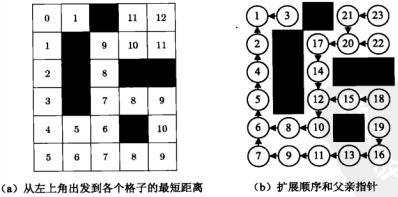
\includegraphics{maze.png}\\
\figcaption{用BFS求迷宫中最短路径}\label{fig:maze}
\end{center}

\subsubsection{代码}
\begin{Codex}[label=maze.c]
#include <stdio.h>
#include <string.h>

#define MAXN 5

// 迷宫的行数,列数
int m = MAXN, n = MAXN;
// 迷宫,0表示空地,1表示障碍物
int map[MAXN][MAXN];

// 四个方向
const char name[4] = { 'U', 'R', 'D', 'L' };
const int dx[4] = { -1, 0, 1, 0 }; // 行
const int dy[4] = { 0, 1, 0, -1 }; // 列

#ifndef __cplusplus
typedef char bool;
#define false 0
#define true 1
#endif

typedef struct state_t {
    int data;
    int action;
    int father;
} state_t;

#define STATE_MAX MAXN*MAXN  /* 状态总数 */

state_t path[STATE_MAX];

void print_action(const int end) {
    if (path[end].father == -1) return;

    print_action(path[end].father);
    putchar(name[path[end].action]);
}

void print_path(const int end) {
    if (path[end].father == -1) {
        printf("(%d, %d)\n", end / n, end % n);
        return;
    }
    print_path(path[end].father);
    printf("(%d, %d)\n", end / n, end % n);
}

int state_hash(const state_t *s);

void history_init();

bool history_contains(const state_t *s);

void history_insert(const state_t *s);

void state_extend_init(const state_t *s);

bool state_extend(const state_t *s, state_t *next);

bool state_is_target(const state_t *s);

typedef state_t queue_elem_t; // 元素的类型
/* 等价于复制粘贴,这里为了节约篇幅,使用include,在OJ上提交时请用复制粘贴 */
#include "queue.c"  /* 见“栈和队列->队列”这节,如果是C++,则使用std::queue */
queue_t q;

int bfs(state_t *start) {
    queue_init(&q, 16);
    history_init();

    start->action = -1;
    start->father = -1;

    path[state_hash(start)] = *start;
    history_insert(start);
    queue_push(&q, *start);

    while (!queue_empty(&q)) {
        const state_t s = queue_front(&q);
        queue_pop(&q);
        state_t next;
        state_extend_init(&s);
        while (state_extend(&s, &next)) {
            if (state_is_target(&next)) {
                queue_uninit(&q);
                return state_hash(&next);
            }
            queue_push(&q, next);
            history_insert(&next);
        }
    }
    queue_uninit(&q);
    return -1;
}

int main(void) {
    int i, j;
    state_t start = {0, -1, -1}; /* 左上角为起点 */
    int end;

    for (i = 0; i < m; i++) {
        for (j = 0; j < n; j++) {
            scanf("%d", &map[i][j]);
        }
    }

    end = bfs(&start);
    print_path(end);
    return 0;
}

/********** functions implement **************/
/* 哈希表容量,要大于状态总数,若存在完美哈希方案,则等于状态总数 */
#define HASH_CAPACITY STATE_MAX
bool visited[HASH_CAPACITY];

int state_hash(const state_t *s) {
    return s->data;
}

void history_init() {
    memset(visited, 0, sizeof(visited));
}

bool history_contains(const state_t *s) {
    return visited[state_hash(s)] == true;
}

void history_insert(const state_t *s) {
    visited[state_hash(s)] = true;
}

int action_cur;
#define ACTION_BEGIN 0
#define ACTION_END 4
/** 扩展点,即当前位置 */
int x, y;

void state_extend_init(const state_t *s) {
    action_cur = ACTION_BEGIN;
    x = s->data / n;
    y = s->data % n;
}

bool state_extend(const state_t *s, state_t *next) {
    while(action_cur < ACTION_END) {
        const int nx = x + dx[action_cur];
        const int ny = y + dy[action_cur];

        if (nx >= 0 && nx < m && ny >= 0 && ny < n && !map[nx][ny]) {
            next->data = nx * n + ny;

            if (!history_contains(next)) { /* 判重 */
                /* 记录路径 */
                next->action = action_cur;
                next->father = state_hash(s);
                path[state_hash(next)] = *next;

                action_cur++;  /* return前别忘了增1 */
                return true;
            }
        }
        action_cur++;
    }
    return false;
}

const state_t END = {24, -1, -1};
bool state_is_target(const state_t *s) {
    return s->data == END.data;
}
\end{Codex}

\subsubsection{相关的题目}
与本题相同的题目:
\begindot
\item 《算法竞赛入门经典》\footnote{刘汝佳,算法竞赛入门经典,清华大学出版社,2009}第108页6.4.2节
\item  POJ 3984 迷宫问题, \myurl{http://poj.org/problem?id=3984}
\myenddot

与本题相似的题目:
\begindot
\item  POJ 2049 Finding Nemo, \myurl{http://poj.org/problem?id=2049}
\myenddot


\section{八数码问题} %%%%%%%%%%%%%%%%%%%%%%%%%%%%%%
\label{subsec:eightDigits}

\subsubsection{描述}
编号为1$\sim$8的8个正方形滑块摆成3行3列,有一个格子空着,如图~\ref{fig:eightDigits}所示。

\begin{center}
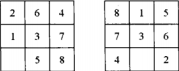
\includegraphics{eight-digits.png}\\
\figcaption{用BFS求迷宫中最短路径}\label{fig:eightDigits}
\end{center}

每次可以把与空格相邻的滑块(有公共边才算相邻)移到空格中,而它原
来的位置就成了新的空格。目标局面固定如下(用$x$表示空格):
\begin{Code}
1 2 3
4 5 6
7 8 x
\end{Code}

给定初始局面,计算出最短的移动路径。

\subsubsection{输入}
用一行表示一个局面,例如下面的这个局面:
\begin{Code}
 1  2  3
 x  4  6
 7  5  8
\end{Code}
可以表示为 1 2 3 x 4 6 7 5 8。 

\subsubsection{输出}
如果有解答,输出一个由四个字母'r','l','u','d'组成的移动路径。
如果没有,输出"unsolvable"。 

\subsubsection{样例输入}
\begin{Code}
2  3  4  1  5  x  7  6  8
\end{Code}

\subsubsection{样例输出}
\begin{Code}
ullddrurdllurdruldr
\end{Code}

\subsubsection{分析}
计算“最短”,很自然的想到BFS。

如何表示一个状态?本题是一个3*3的棋盘,状态有9!个,可以用一个32位整数表示,但15!已经超过32位整数的
范围,21!超过了64位整数的范围,因此4*4的棋盘可以用一个64位整数表示。超过4*4的棋盘,则无法用整数来
表示了,可以用一个数组来表示。

如何判重?用哈希表或者集合。哈希表的话,由于C++ STL 还没有 \fn{std::hashset},
需要自己实现哈希表,然后由于本题的特殊性,存在一种完美哈希(perfect hashing)方案。集合可以直接
使用\fn{std::set}。总结起来,有以下三个方法:
\begindot
\item 把排列变成整数,这是一种完美哈希,即不存在冲突
\item 用普通的哈希表,这种方法通用一些,速度也略慢。手工实现哈希表,把哈希值相同的组成一个单链表,
\item 用 \fn{std::set} 实现判重,代码最短,速度也最慢(本题用这个方法会TLE)。建议把该方法作为“跳板”,
先写一个STL版的程序,确保主算法正确,然后把\fn{std::set}替换成自己写的哈希表。
\myenddot

此题更优的解法还有双向BFS(见\S \ref{sec:biBFS}),A*算法(见\S \ref{sec:astar})。

\subsubsection{代码}

方案1,完美哈希,使用康托展开。

\begin{Codex}[label=eight_digits_bfs.c]
/* POJ 1077 Eight, http://poj.org/problem?id=1077 */
#include <stdio.h>
#include <string.h>

#define DIGITS 9 // 棋盘中数字的个数,也是变进制数需要的位数
#define     MATRIX_EDGE 3       // 棋盘边长

/***** 一些常量 *****/
const int SPACE_NUMBER = 0; // 空格对应着数字 0
// 上下左右四个方向
const int dx[] = {-1, 1, 0, 0};
const int dy[] = {0, 0, -1, 1};
const char name[] = { 'u', 'd', 'l', 'r' };

#ifndef __cplusplus
typedef char bool;
#define false 0
#define true 1
#endif

typedef char int8_t;

/**
 * @strut 状态
 */
typedef struct state_t {
    int8_t data[DIGITS];  /** 状态的数据. */
    int action; /* 由父状态移动到本状态的动作 */
    int father; /* 父状态在path[]中的下标,也即父状态的哈希值 */
    int count;  /** 所花费的步骤数(也即路径长度-1) */
} state_t;

// 3x3的棋盘,状态最多有 9!种
#define STATE_MAX 362880  /* 状态总数 */

state_t path[STATE_MAX+1];

/**
 * @brief 打印动作序列.
 * @param[in] end 终点状态的哈希值
 * @return 父状态
 */
void print_action(const int end) {
    if (path[end].father == -1) return;

    print_action(path[end].father);
    putchar(name[path[end].action]);
}

int state_hash(const state_t *s);

void history_init();

bool history_contains(const state_t *s);

void history_insert(const state_t *s);

void state_extend_init(const state_t *s);

bool state_extend(const state_t *s, state_t *next);

bool state_is_target(const state_t *s);

typedef state_t queue_elem_t; // 元素的类型
/* 等价于复制粘贴,这里为了节约篇幅,使用include,在OJ上提交时请用复制粘贴 */
#include "queue.c"  /* 见“栈和队列->队列”这节,如果是C++,则使用std::queue */
// 队列
queue_t q;

int bfs(state_t *start) {
    queue_init(&q, 16);
    history_init();

    start->action = -1;
    start->father = -1;
    start->count = 0;

    path[state_hash(start)] = *start;
    history_insert(start); // 千万别忘记了标记此处的访问记录
    queue_push(&q, *start);

    while (!queue_empty(&q)) {
        const state_t s = queue_front(&q);
        state_t next;
        queue_pop(&q);

        state_extend_init(&s);
        while (state_extend(&s, &next)) {
            if (state_is_target(&next)) {
                // printf("%d\n", next.count);
                queue_uninit(&q);
                return state_hash(&next);
            }
            queue_push(&q, next);
            history_insert(&next);
        }
    }
    queue_uninit(&q);
    return -1;
}

/**
 * @brief 输入.
 * @return 无
 */
void input(state_t *start) {
    int ch, i;
    for (i = 0; i < DIGITS; ++i) {
        do {
            ch = getchar();
        } while ((ch != EOF) && ((ch < '1') || (ch > '8')) && (ch != 'x'));
        if (ch == EOF) return;
        if (ch == 'x') start->data[i] = 0; // x 映射成数字 0
        else           start->data[i] = ch - '0';
    }
}

/** for wikioi 1225 */
void input1(state_t *start) {
    int i, n;
    scanf("%d", &n);

    /* 将整数转化为棋盘 */
    for(i = DIGITS-1; i >= 0; i--) {
        start->data[i] = n % 10;
        n /= 10;
    }
}

int main(void) {
    state_t start;
    int end; /* 目标状态在path[]中的下标 */
    input(&start);

    end = bfs(&start);

    print_action(end);
    printf("\n");
    return 0;
}

/********** functions implement **************/

/********** 方案1,完美哈希,使用康托展开 **************/

// 9 位变进制数(空格)能表示0到(9!-1)内的所有自然数,恰好有9!个,
// 与状态一一对应,因此可以把状态一一映射到一个9位变进制数

// 9 位变进制数,每个位数的单位,0!~8!
const int fac[] = {40320, 5040, 720, 120, 24, 6, 2, 1, 1};
/* 哈希表容量,要大于状态总数,若存在完美哈希方案,则等于状态总数 */
#define HASH_CAPACITY STATE_MAX

bool visited[HASH_CAPACITY];

int state_hash(const state_t *s) {
    int i, j;
    int key = 0;
    for (i = 0; i < DIGITS; i++) {
        int cnt = 0;  /* 逆序数 */
        for (j = i + 1; j < DIGITS; j++) if (s->data[i] > s->data[j]) cnt++;
        key += fac[i] * cnt;
    }
    return key;
}

void history_init() {
    memset(visited, 0, sizeof(visited));
}

bool history_contains(const state_t *s) {
    return visited[state_hash(s)] == true;
}

void history_insert(const state_t *s) {
    visited[state_hash(s)] = true;
}

int action_cur;
#define ACTION_BEGIN 0
#define ACTION_END 4

/* 扩展点,即0的位置 */
int z;

void state_extend_init(const state_t *s) {
    action_cur = ACTION_BEGIN;
    for (z = 0; z < DIGITS; z++) {
        if (s->data[z] == SPACE_NUMBER) {
            break;  // 找 0 的位置
        }
    }
}

bool state_extend(const state_t *s, state_t *next) {
    const int x = z / MATRIX_EDGE; // 行
    const int y = z % MATRIX_EDGE; // 列

    while (action_cur < ACTION_END) {
        const int newx = x + dx[action_cur];
        const int newy = y + dy[action_cur];
        const int newz = newx * MATRIX_EDGE + newy;

        if (newx >= 0 && newx < MATRIX_EDGE && newy >= 0 &&
                newy < MATRIX_EDGE) { // 没有越界
            *next = *s;
            next->data[newz] = SPACE_NUMBER;
            next->data[z] = s->data[newz];
            next->count = s->count + 1;
            if (!history_contains(next)) { /* 判重 */
                next->action = action_cur;
                next->father = state_hash(s);
                /* 记录路径 */
                path[state_hash(next)] = *next;
                action_cur++; /* return前别忘了增1 */
                return true;
            }
        }
        action_cur++;
    }
    return false;
}

// 目标状态
const state_t END = {{1, 2, 3, 4, 5, 6, 7, 8, 0}, -1, -1};
// for wikioi 1225
const state_t END1 = {{1, 2, 3, 8, 0, 4, 7, 6, 5}, -1, -1};

bool state_is_target(const state_t *s) {
    return memcmp(s->data, END.data, DIGITS * sizeof(int8_t)) == 0;
}
\end{Codex}

方案2,不知道是否存在完美哈希方案,但能够预估状态个数的上限,用树双亲表示法存储路径,用自己实现的哈希表判重。

\begin{Codex}[label=eight_digits_bfs2.c]
/* POJ 1077 Eight, http://poj.org/problem?id=1077 */
#include <stdio.h>
#include <string.h>
#include <assert.h>

#define DIGITS 9 // 棋盘中数字的个数,也是变进制数需要的位数
#define     MATRIX_EDGE 3       // 棋盘边长

/***** 一些常量 *****/
const int SPACE_NUMBER = 0; // 空格对应着数字 0
// 上下左右四个方向
const int dx[] = {-1, 1, 0, 0};
const int dy[] = {0, 0, -1, 1};
const char name[] = { 'u', 'd', 'l', 'r' };

#ifndef __cplusplus
typedef char bool;
#define false 0
#define true 1
#endif

typedef char int8_t;

/**
 * @strut 状态
 */
typedef struct state_t {
    int8_t data[DIGITS];  /** 状态的数据. */
    int action; /* 由父状态移动到本状态的动作 */
    int index;  /** 本状态在path[]中的下标 */
    int father; /** 父状态在path[]中的下标 */
    int count;  /** 所花费的步骤数(也即路径长度-1) */
} state_t;

// 3x3的棋盘,状态最多有 9!种
#define STATE_MAX 362880  /* 状态总数 */

state_t path[STATE_MAX+1];
int path_index = 0;

/**
 * @brief 打印动作序列.
 * @param[in] end 终点状态的哈希值
 * @return 父状态
 */
void print_action(const int end) {
    if (path[end].father == -1) return;

    print_action(path[end].father);
    putchar(name[path[end].action]);
}

void history_init();

bool history_contains(const state_t *s);

void history_insert(const state_t *s);

void state_extend_init(const state_t *s);

bool state_extend(const state_t *s, state_t *next);

bool state_is_target(const state_t *s);

typedef state_t queue_elem_t; // 元素的类型
/* 等价于复制粘贴,这里为了节约篇幅,使用include,在OJ上提交时请用复制粘贴 */
#include "queue.c"  /* 见“栈和队列->队列”这节,如果是C++,则使用std::queue */
// 队列
queue_t q;

int bfs(state_t *start) {
    queue_init(&q, 16);
    history_init();

    start->action = -1;
    start->index = path_index++;
    start->father = -1;
    start->count = 0;

    path[start->index] = *start;
    history_insert(start); // 千万别忘记了标记此处的访问记录
    queue_push(&q, *start);

    while (!queue_empty(&q)) {
        const state_t s = queue_front(&q);
        state_t next;
        queue_pop(&q);

        state_extend_init(&s);
        while (state_extend(&s, &next)) {
            if (state_is_target(&next)) {
                // printf("%d\n", next.count);
                queue_uninit(&q);
                return next.index;
            }
            queue_push(&q, next);
            history_insert(&next);
        }
    }
    queue_uninit(&q);
    return -1;
}

/**
 * @brief 输入.
 * @return 无
 */
void input(state_t *start) {
    int ch, i;
    for (i = 0; i < DIGITS; ++i) {
        do {
            ch = getchar();
        } while ((ch != EOF) && ((ch < '1') || (ch > '8')) && (ch != 'x'));
        if (ch == EOF) return;
        if (ch == 'x') start->data[i] = 0; // x 映射成数字 0
        else           start->data[i] = ch - '0';
    }
}

/** for wikioi 1225 */
void input1(state_t *start) {
    int i, n;
    scanf("%d", &n);

    /* 将整数转化为棋盘 */
    for(i = DIGITS-1; i >= 0; i--) {
        start->data[i] = n % 10;
        n /= 10;
    }
}

int main(void) {
    state_t start;
    int end;
    input(&start);

    end = bfs(&start);

    print_action(end);
    printf("\n");
    return 0;
}

/********** functions implement **************/

/********** 方案2 不知道完美哈希方案,自己实现哈希表 **************/
#define HASH_CAPACITY  10000000  /* 哈希表容量,要大于状态总数 */

int head[HASH_CAPACITY];
int next[STATE_MAX];

int state_hash(const state_t *s) {
    int i;
    int ret = 0;
    for(i = 0; i < DIGITS; i++) ret = ret * 10 + s->data[i];
    return ret % HASH_CAPACITY;
}

void history_init() {
    memset(head, 0, sizeof(head));
    memset(next, 0, sizeof(next));
}

bool history_contains(const state_t *s) {
    const int h = state_hash(s);
    int u = head[h]; // 从表头开始查找单链表
    while(u) {
        // 找到了
        if(memcmp(path[u].data, s->data,
                DIGITS * sizeof(int8_t)) == 0) return true;
        u = next[u]; // 顺着链表继续找
    }
    return false;
}

void history_insert(const state_t *s) {
    const int h = state_hash(s);
    int u = head[h]; // 从表头开始查找单链表
    while(u) {
        // 找到了,插入失败
        if(memcmp(path[u].data, path[s->index].data,
                sizeof(DIGITS * sizeof(int8_t))) == 0) return;
        u = next[u]; // 顺着链表继续找
    }
    assert(head[h] >= 0);
    next[s->index] = head[h];  /* 插入到首节点前面,头查法 */
    head[h] = s->index;
    return;
}

int action_cur;
#define ACTION_BEGIN 0
#define ACTION_END 4

/* 扩展点,即0的位置 */
int z;

void state_extend_init(const state_t *s) {
    action_cur = ACTION_BEGIN;
    for (z = 0; z < DIGITS; z++) {
        if (s->data[z] == SPACE_NUMBER) {
            break;  // 找 0 的位置
        }
    }
}

bool state_extend(const state_t *s, state_t *next) {
    const int x = z / MATRIX_EDGE; // 行
    const int y = z % MATRIX_EDGE; // 列

    while (action_cur < ACTION_END) {
        const int newx = x + dx[action_cur];
        const int newy = y + dy[action_cur];
        const int newz = newx * MATRIX_EDGE + newy;

        next->count = s->count + 1;
        if (newx >= 0 && newx < MATRIX_EDGE && newy >= 0 &&
                newy < MATRIX_EDGE) { // 没有越界
            *next = *s;
            next->data[newz] = SPACE_NUMBER;
            next->data[z] = s->data[newz];

            if (!history_contains(next)) { /* 判重 */
                next->action = action_cur;
                next->index = path_index++;
                next->father = s->index;
                /* 记录路径 */
                path[next->index] = *next;
                action_cur++; /* return前别忘了增1 */
                return true;
            }
        }
        action_cur++;
    }
    return false;
}

// 目标状态
const state_t END = {{1, 2, 3, 4, 5, 6, 7, 8, 0}, -1, -1};
// for wikioi 1225
const state_t END1 = {{1, 2, 3, 8, 0, 4, 7, 6, 5}, -1, -1};

bool state_is_target(const state_t *s) {
    return memcmp(s->data, END.data, DIGITS * sizeof(int8_t)) == 0;
}
\end{Codex}

方案3,不知道完美哈希方案,但能够预估状态个数的上限制,用树双亲表示法存储路径,用标准库的哈希表判重。

\begin{Codex}[label=eight_digits_bfs3.cpp]
//前面的代码与方案2一摸一样
//...

/********** 方案3 不知道完美哈希方案,使用标准库的哈希表 **************/

// 重载 state_t 的 == 操作符
typedef struct state_t {
    int8_t data[DIGITS];  /** 状态的数据. */
    int action; /* 由父状态移动到本状态的动作 */
    int index;  /** 本状态在path[]中的下标 */
    int father; /** 父状态在path[]中的下标 */
    int count;  /** 所花费的步骤数(也即路径长度-1) */

    bool operator==(const state_t& other) const {
        return memcmp(data, other.data, DIGITS * sizeof(int8_t)) == 0;
    }
} state_t;

#include <unordered_set>

// 定制一个哈希函数
namespace std {
template<> struct hash<state_t> {
    size_t operator()(const state_t & x) const {
        int i;
        int ret = 0;
        for (i = 0; i < DIGITS; i++)
            ret = ret * 10 + x.data[i];
        return ret;
    }
};
}

std::unordered_set<state_t> visited;

void history_init() {
    visited.clear();
}

bool history_contains(const state_t *s) {
    return visited.count(*s) > 0;
}

void history_insert(const state_t *s) {
    visited.insert(*s);
}

//...
//后面的代码也与方案2一摸一样
\end{Codex}

\subsubsection{相关的题目}
与本题相同的题目:
\begindot
\item 《算法竞赛入门经典》\footnote{刘汝佳,算法竞赛入门经典,清华大学出版社,2009} 第131页7.5.3节
\item  POJ 1077 Eight, \myurl{http://poj.org/problem?id=1077}
\item  wikioi 1225 八数码难题, \myurl{http://www.wikioi.com/problem/1225/}
\myenddot

与本题相似的题目:
\begindot
\item  POJ 2893 M × N Puzzle, \myurl{http://poj.org/problem?id=2893}
\myenddot


\section{四子连棋} %%%%%%%%%%%%%%%%%%%%%%%%%%%%%%

\subsubsection{描述}
在一个4*4的棋盘上摆放了14颗棋子,其中有7颗白色棋子,7颗黑色棋子,有两个空白地带,任何一颗黑白
棋子都可以向上下左右四个方向移动到相邻的空格,这叫行棋一步,黑白双方交替走棋,任意一方可以先走,
如果某个时刻使得任意一种颜色的棋子形成四个一线(包括斜线),这样的状态为目标棋局。

\subsubsection{输入}
一个4*4的初始棋局,黑棋子用B表示,白棋子用W表示,空格地带用O表示。

\subsubsection{输出}
移动到目标棋局的最少步数。

\subsubsection{样例输入}
\begin{Code}
BWBO
WBWB
BWBW
WBWO
\end{Code}

\subsubsection{样例输出}
\begin{Code}
5
\end{Code}

\subsubsection{分析}
求最少步数,很自然的想到广搜。

如何表示一个状态?用一个二维数组\fn{int board[4][4]}表示,还需要记录该状态是由白子还是黑子移动而导致的,走到该状态已经花费的步数。

如何扩展节点?每一步,从队列弹出一个状态,两个空格都可以向四个方向扩展,把得到的状态入队列。

如何判重?棋盘用二维矩阵存储,用0表示空格,1表示黑色,2表示白色,所以最后可以看成一个16位的三进制数。
用这个数作为棋盘的编码,就可以用来判重了。注意,本题要黑白交替走,所以我们要区分状态是由白子还是黑子移动而导致的。

可以用C++的\fn{std::map}来判重,
\begin{Code}
/* history[0]记录白子的历史,history[1]记录黑子的历史. */
std::map<int, bool> history[2];
\end{Code}

也可以开一个大数组当做哈希表,
\begin{Code}
#define HASH_MOD 43036875 /* hash表大小 */
/* history[0]记录白子的历史,history[1]记录黑子的历史. */
bool history[2][HASH_MOD];
\end{Code}

\subsubsection{代码}
\begin{Codex}[label=four_adjacent.c]
/** wikioi 1004 四子连棋  , http://www.wikioi.com/problem/1004 */
#include <stdio.h>
#include <string.h>

#define LEN 4   /* 边长 */

/* 右,左,上,下(左下角为坐标原点)*/
const int dx[] = { 1, -1, 0, 0 };
const int dy[] = { 0, 0, 1, -1 };


#ifndef __cplusplus
typedef char bool;
#define false 0
#define true 1
#endif

/**
 * @strut 状态
 */
typedef struct state_t {
    // 状态的数据
    int board[LEN][LEN]; /* 棋局,1表示黑子,2表示白子,0表示空白 */
    int color; /* 本状态是由白子还是黑子移动而导致的 */
    int count;  /** 所花费的步骤数(也即路径长度-1),求路径长度时需要 */
} state_t;

/**
 * @brief 计算状态的哈希值。
 * 棋盘用二维矩阵存储,用0表示空格,1表示黑色,2表示白色,所以最后可以看成
 * 一个16位的三进制数。最大为
 * 2222
 * 2221
 * 1111
 * 1100
 * 值为 43036875。
 * @return 棋盘所表示的三进制数转化为十进制数
 */
//TODO:共C16 7×C9 2个状态,用类似康托的方法储存
int state_hash(const state_t *s);

void history_init();

bool history_contains(const state_t *s);

void history_insert(const state_t *s);

void state_extend_init(const state_t *s);

bool state_extend(const state_t *s, state_t *next);

bool state_is_target(const state_t *s);

typedef state_t queue_elem_t; // 元素的类型
/* 等价于复制粘贴,这里为了节约篇幅,使用include,在OJ上提交时请用复制粘贴 */
#include "queue.c"  /* 见“栈和队列->队列”这节,如果是C++,则使用std::queue */
// 队列
queue_t q;

void bfs(state_t *start) {
    queue_init(&q, 16);
    history_init();

    start->count = 0;
    start->color = 1;

    history_insert(start);
    queue_push(&q, *start);

    start->color = 2;

    history_insert(start); // 千万别忘记了标记此处的访问记录
    queue_push(&q, *start);

    while (!queue_empty(&q)) {
        const state_t s = queue_front(&q);
        state_t next;
        queue_pop(&q);

        state_extend_init(&s);
        while (state_extend(&s, &next)) {
            if (state_is_target(&next)) {
                printf("%d\n", next.count);
                queue_uninit(&q);
                return;
            }
            queue_push(&q, next);
            history_insert(&next);
        }
    }
    queue_uninit(&q);
}

int main() {
    int i, j;
    char s[LEN + 1];
    state_t start;

    for (i = 0; i < LEN; i++) {
        scanf("%s", s);
        for (j = 0; j < LEN; j++) {
            if (s[j] == 'B') start.board[i][j] = 1;
            else if (s[j] == 'W') start.board[i][j] = 2;
            else start.board[i][j] = 0;
        }
    }

    bfs(&start);
    queue_uninit(&q);
    return 0;
}

/************ functions implement ************/

/* 哈希表容量,要大于状态总数,若存在完美哈希方案,则等于状态总数 */
#define HASH_CAPACITY 43036875

/** 哈希表,标记状态是否已访问过。
 * visited[0]记录白子的历史,visited[1]记录黑子的历史.
 */
bool visited[2][HASH_CAPACITY];

#define RADIX 3 /* 三进制 */

int state_hash(const state_t *s) {
    int i, j;
    int ret = 0;

    for (i = 0; i < LEN; i++) {
        for (j = 0; j < LEN; j++) {
            ret = ret * RADIX + s->board[i][j];
        }
    }
    return ret;
}

void history_init() {
    memset(visited[0], 0, sizeof(sizeof(bool) * HASH_CAPACITY));
    memset(visited[1], 0, sizeof(sizeof(bool) * HASH_CAPACITY));
}

bool history_contains(const state_t *s) {
    return visited[s->color - 1][state_hash(s)] == true;
}

void history_insert(const state_t *s) {
    visited[s->color - 1][state_hash(s)] = true;
}

/* 扩展的时候,先定空格,再定方向 */
/* 记录当前方向,例如action_cur[0]记录了第一个空格,当前在扩展哪个方向
 */
int action_cur[2];
#define ACTION_BEGIN 0
#define ACTION_END 4

typedef struct point_t {
    int x, y;
} point_t;

/* 记录当前在扩展哪一个空格,值为0或1 */
int space_cur;
/* 两个空格的位置 */
point_t extend_pos[2];

void state_extend_init(const state_t *s) {
    int i, j, k;
    action_cur[0] = ACTION_BEGIN;
    action_cur[1] = ACTION_BEGIN;
    space_cur = 0;

    k = 0;
    // 寻找两个空白的格子的位置
    for (i = 0; i < LEN; i++) {
        for (j = 0; j < LEN; j++) {
            if (s->board[i][j] == 0) {
                extend_pos[k].x = i;
                extend_pos[k].y = j;
                k++;
            }
        }
    }
}

bool state_extend(const state_t *s, state_t *next) {
    int i;

    for (i = 0; i < 2; i++) { /* 先第一个空格,再第二个空格 */
        while (action_cur[i] < ACTION_END) {
            const int x = extend_pos[i].x;
            const int y = extend_pos[i].y;
            int nextx = x + dx[action_cur[i]];
            int nexty = y + dy[action_cur[i]];
            *next = *s;
            next->count = s->count + 1;
            next->color = 3 - s->color;

            if (nextx >= 0 && nextx < LEN && nexty >= 0 && nexty < LEN
                    /* 必须黑白交替走 */
                    && next->color == s->board[nextx][nexty]) {
                /* swap */
                {
                    int temp = next->board[x][y];
                    next->board[x][y] = next->board[nextx][nexty];
                    next->board[nextx][nexty] = temp;
                }

                if (!history_contains(next)) { /* 判重 */
                    action_cur[i]++; /* return前别忘了增1 */
                    return true;
                }
            }
            action_cur[i]++;
        }
    }
    return false;
}

bool state_is_target(const state_t *s) {
    int i, j;
    for (i = 0; i < LEN; i++) {  /* 逐行检查 */
        int flag = 1;  /* 某一行全是同一颜色 */
        for (j = 1; j < LEN; j++)
            if (s->board[i][j - 1] != s->board[i][j])
                flag = 0;
        if (flag)
            return 1;
    }
    for (j = 0; j < LEN; j++) { //逐列检查
        int flag = 1;  /* 某一行全是同一颜色 */
        for (i = 1; i < LEN; i++)
            if (s->board[i][j] != s->board[i - 1][j]) flag = 0;
        if (flag) return 1;
    }
    /* 斜线 */
    if (s->board[0][0] == s->board[1][1] && s->board[1][1] == s->board[2][2]
            && s->board[2][2] == s->board[3][3])
        return 1;
    if (s->board[0][3] == s->board[1][2] && s->board[1][2] == s->board[2][1]
            && s->board[2][1] == s->board[3][0])
        return 1;
    return 0;
}
\end{Codex}

\subsubsection{相关的题目}
与本题相同的题目:
\begindot
\item  wikioi 1004 四子连棋, \myurl{http://www.wikioi.com/problem/1004/}
\myenddot

与本题相似的题目:
\begindot
\item  None
\myenddot


\section{双向BFS} %%%%%%%%%%%%%%%%%%%%%%%%%%%%%%
\label{sec:biBFS}


\subsection{八数码问题}
题目见 \S \ref{subsec:eightDigits}。

\subsubsection{代码}

\begin{Codex}[label=eight_digits_bibfs.c]

\end{Codex}


\section{A*算法} %%%%%%%%%%%%%%%%%%%%%%%%%%%%%%
\label{sec:astar}

\textbf{A*算法 = 宽搜 + 优先队列}

\subsection{八数码问题}
题目见 \S \ref{subsec:eightDigits}。

\subsubsection{代码}
\begin{Codex}[label=eight_digits_astar.c]
/** POJ 1077 Eight, http://poj.org/problem?id=1077
 简单解释几个要点,便于理解代码.
 1. 怎么判断是否有解?只要计算出的逆序个数总和为奇数,该数据必然无解
 2. 如何判断某一状态是否到过?本题存在一种完美哈希方案,即用康托展开。
    详见 http://128kj.iteye.com/blog/1699795
    2.1.将一个状态视为数字 0-8 的一个排列,将此排列转化为序数,作为此状
 态的 HASH 值。0表示空格.转化算法此处不再赘述。

    2.2.排列转化为序数,用序数作为hash值
    例,1 2 3 这三个数字的全排列,按字典序,依次为
 123 -- 0
 132 -- 1
 213 -- 2
 231 -- 3
 312 -- 4
 321 -- 5
 其中,左侧为排列,右侧为其序数。

 3.使用数据结构 —— 堆,加速挑选最优值。

 4.函数 g 的计算,此状态在搜索树中已经走过的路径的节点数.

 5.估价函数 h ,采用曼哈顿距离, 见代码 calcH 函数。曼哈顿距离的定义是,
 假设有两个点(x1,y1),(x2,y2),则曼哈顿距离L1=|x1-x2| + |y1-y2|
 */
#include <stdio.h>
#include <string.h>
#include <stdlib.h>

// 3x3的棋盘,状态最多有 9!种
// 8位变进制数(空格)能表示0到(9!-1)内的所有自然数,恰好有9!个,
// 与状态一一对应,因此可以把状态一一映射到一个8位变进制数
#define     MAX         362880

#define DIGITS 9 // 棋盘中数字的个数,也是变进制数需要的位数
#define     MATRIX_EDGE 3       // 棋盘边长

#define     MOD         10      // 按十取模

typedef struct {
    int state; // 状态
    int parent;     // 父状态
    int flag;   // -1 表示已经展开过了closed,0表示死节点,1 表示还未展开, open
    int g, h, f; // 三个评估函数
    char choice;  // 左右上下四个方向移动,见全局常量 DI DJ DC
} state_t;

state_t states[MAX];  // 全局的一条状态变化路径

int  startIndex, goalIndex; // 开始状态,目标状态对应的hash值

// 目标状态
const int GOAL = 123456780;
// 每个数字在棋盘中的位置,例如0,在(2,2)=8这个位置上
int GOAL_POS[DIGITS];
const int SPACE_NUMBER = 0; // 空格对应着数字 0

// 上下左右四个方向
const int DI[] = {-1, 1, 0, 0};
const int DJ[] = {0, 0, -1, 1};
const char DC[] = { 'u', 'd', 'l', 'r' };

// 9 位变进制数,每个位数的单位,0!~8!
const int fac[] = {40320, 5040, 720, 120, 24, 6, 2, 1, 1};

/* 计算GOAL_POS */
void calc_goal_pos() {
    int cur = GOAL;
    int i;
    for (i = DIGITS-1; i >= 0 ; i--) {
        int digit = cur % MOD;
        GOAL_POS[digit] = i;
        cur /= MOD;
    }
}

/**
 * @brief 计算状态的hash值,这里用康托展开,是完美哈希.
 *
 * @param[in] s 当前状态
 * @return 序数,作为hash值
 */
int hash(int s) {
    int i, j;
    int d[DIGITS];
    int key = 0;

    for(i = DIGITS - 1; i >=0; i--) {
        d[i] = s % MOD;
        s /= MOD;
    }

    for (i = 0; i < DIGITS; i++) {
        int c = 0; // 逆序数
        for (j = i + 1; j < DIGITS; j++) {
            if(d[j] < d[i]) {
                c++;
            }
        }
        key += c * fac[i];
    }

    return key;
}


/**
 * 估价函数h。
 * @param s 状态
 * @return 预估代价
 */
int calcH(int s) {
    int i;
    int h = 0;

    for (i = DIGITS - 1; i >= 0; --i) {
        const int p = s % 10;
        s /= 10;
        // 曼哈顿距离
        h += abs(i / MATRIX_EDGE - GOAL_POS[p] / MATRIX_EDGE) +
            abs(i % MATRIX_EDGE - GOAL_POS[p] % MATRIX_EDGE);
    }
    return h;
}

/**
 * @brief 输入.
 * @return  成功返回数字,失败返回0
 * @remark 《算法竞赛入门经典》第131页7.5.3节,是用0表示空格,
 * POJ 1077是用'x'表示空格,前者简化了一点,POJ 1077还需要把'x'映射成0
 */
int input() {
    int ch, i;
    int start = 0;
    for (i = 0; i < DIGITS; ++i) {
        do {
            ch = getchar();
        } while ((ch != EOF) && ((ch < '1') || (ch > '8')) && (ch != 'x'));
        if (ch == EOF) return 0;
        if (ch == 'x') start = start * MOD + SPACE_NUMBER; // x 映射成数字 0
        else             start = start * MOD + ch - '0';
    }
    return start;
}

/** for wikioi 1225 */
int input1() {
    int start;
    scanf("%d", &start);
    return start;
}

/**
 * 计算一个排列的逆序数,0 除外.
 */
int inversion_count(int permutation) {
    int i, j;
    int d[DIGITS];
    int c = 0; // 逆序数

    for(i = DIGITS - 1; i >=0; i--) {
        d[i] = permutation % MOD;
        permutation /= MOD;
    }

    for (i = 1; i < DIGITS; i++)  if (d[i] != SPACE_NUMBER) {
        for (j = 0; j < i; j++) {
            if(d[j] != SPACE_NUMBER) {
                if (d[j] > d[i]) {
                    c++;
                }
            }
        }
    }
    return c;
}

/**
 * 判断是否无解.
 *
 * 求出除0之外所有数字的逆序数之和,也就是每个数字后面比它小的数字的个数的和,
 * 称为这个状态的逆序。
 *
 * 若起始状态和目标状态的逆序数奇偶性相同,则可相互到达,否则不可相互到达。
 *
 * @param s 目标状态
 * @return 1表示有解,0表示无解
 */
int solvable(const int s) {
    return (inversion_count(s) + inversion_count(GOAL)) % 2 == 0;
}

// 存放 next()的输出结果
char choice[4]; // 四个防线
int nextIndex[4]; // 接下来的四个状态

/*
 * @brief 向四个方向扩展
 * @param[in] s 状态
 * @return 无
 */
void next(int s) {
    int i, j, k;
    int p[MATRIX_EDGE][MATRIX_EDGE]; // 一个状态对应的矩阵
    int i0, j0;  // 空格位置

    for (i = MATRIX_EDGE - 1; i >= 0; i--) {
        for (j = MATRIX_EDGE - 1; j >= 0; j--) {
            p[i][j] = s % MOD;
            s /= MOD;
            if (p[i][j] == SPACE_NUMBER) {
                i0 = i;
                j0 = j;
            }
        }
    }
    // 向四个方向探索
    for (k = 0; k < 4; ++k) {
        const int sx = i0 + DI[k]; // 空格的新位置(sx, sy)
        const int sy = j0 + DJ[k];
        if ((sx >= 0) && (sx < 3) && (sy >= 0) && (sy < 3)) {
            int key;
            p[i0][j0] = p[sx][sy];
            p[sx][sy] = SPACE_NUMBER;
            // 移动空格后,计算新的状态
            s = 0;
            for (i = 0; i < MATRIX_EDGE; i++)
                for (j = 0; j < MATRIX_EDGE; j++)
                    s = s * MOD + p[i][j];
            p[sx][sy] = p[i0][j0]; // 将矩阵还原,(i0, j0)可以不管

            key = nextIndex[k] = hash(s);
            choice[k] = DC[k];
            if (states[key].state == 0) { // 该状态还没有出现过
                states[key].state = s;
                states[key].h = calcH(s);
            }
        } else {// 越界了
            nextIndex[k] = -1;
        }
    }
}

/** 状态的比较函数 */
int cmp_state(const int *x, const int *y) {
    return states[*x].f - states[*y].f;
}

/* 等价于复制粘贴,这里为了节约篇幅,使用include,在OJ上提交时请用复制粘贴 */
#include "heap.c"  /* 见“树->堆”这节 */

heap_t heap;
int heapIndex[MAX + 4]; // 状态 x 在heap中的下标

/**
 * @brief A*搜索
 * @param[in] start 初始状态
 * @return 如果无解,返回0,如果有解返回1
 */
int astar(const int start) {
    int i, j, k, ng, nf;
    if (!solvable(start)) return 0;

    startIndex = hash(start);
    goalIndex  = hash(GOAL);
    if (start == GOAL) return 1;

    memset(states, 0, sizeof(states));
    states[startIndex].state = start;
    states[startIndex].flag    = 1;
    states[startIndex].g       = 0;
    states[startIndex].h       = states[startIndex].f = calcH(start);

    heap_push(&heap, startIndex);
    while(!heap_empty(&heap)) {
        i = heap_top(&heap); heap_pop(&heap);
        if (i == goalIndex) return 1; // 找到目标,返回

        states[i].flag = -1;
        ng = states[i].g + 1;
        next(states[i].state);
        for (k = 0; k < 4; ++k) {
            j = nextIndex[k];
            if (j < 0) continue;
            nf = ng + states[j].h;
            if ((states[j].flag == 0) || ((states[j].flag == 1) &&
                (nf < states[j].f))) {
                states[j].parent = i;
                states[j].choice = choice[k];
                states[j].g    = ng;
                states[j].f    = nf;
                if (states[j].flag > 0) {
                    heap_sift_up(&heap, heapIndex[j]);
                    heap_sift_down(&heap, heapIndex[j]);
                } else {
                    heap_push(&heap, j);
                    states[j].flag = 1;
                }
            }
        }
    }
    return 0;
}

/* 等价于复制粘贴,这里为了节约篇幅,使用include,在OJ上提交时请用复制粘贴 */
#include "stack.c"  /* 见“栈和队列->栈”这节 */

/**
 * @brief 打印移动序列.
 * @return 无
 */
void output() {
    int i;
    stack_t stack;
    stack_init(&stack, MAX);

    for (i = goalIndex; i != startIndex; i = states[i].parent) {
        stack_push(&stack, states[i].choice);
    }
    while(!stack_empty(&stack)) {
        printf("%c", stack_top(&stack));
        stack_pop(&stack);
    }

    printf("\n");
    stack_uninit(&stack);
}

/**
 * @brief 打印棋盘的每次变化.
 * @return 无
 */
void output1() {
    int i;
    int d[DIGITS];
    stack_t stack;
    stack_init(&stack, MAX);

    for (i = goalIndex; i != startIndex; i = states[i].parent) {
        stack_push(&stack, states[i].state);
    }
    stack_push(&stack, states[startIndex].state);

    while(!stack_empty(&stack)) {
        stack_elem_t tmp = stack_top(&stack);
        stack_pop(&stack);
        for(i = DIGITS - 1; i >=0; i--) {
            d[i] = tmp % MOD;
            tmp /= MOD;
        }
        for(i = 0; i < DIGITS; i++) {
            if((i + 1) % MATRIX_EDGE == 0) {
                printf("%d\n", d[i]);
            } else {
                printf("%d ", d[i]);
            }
        }
        printf("\n");
    }
    stack_uninit(&stack);
}

int main() {
    calc_goal_pos();
    const int start = input();
    heap_init(&heap, MAX + 4, cmp_state);

    if (astar(start))  output();
    else printf("no solution\n");

    heap_uninit(&heap);
    return 0;
}
\end{Codex}

\chapter{深度优先搜索}


\section{四色问题} %%%%%%%%%%%%%%%%%%%%%%%%%%%%%%

\subsubsection{描述}
给定$N(N \leq 8)$个点的地图,以及地图上各点的相邻关系,请输出用4种颜色将地图涂色的所有方案数(要求相邻两点不能涂成相同的颜色)。

数据中0代表不相邻,1代表相邻。

\subsubsection{输入}
第一行一个整数$N$,代表地图上有$N$个点。

接下来$N$行,每行$N$个整数,每个整数是0或者1。第i行第j列的值代表了第i个点和第j个点之间是相邻的还是不相邻,相邻就是1,不相邻就是0。我们保证a[i][j] = a[j][i]。

\subsubsection{输出}
染色的方案数

\subsubsection{样例输入}
\begin{Code}
8
0 0 0 1 0 0 1 0 
0 0 0 0 0 1 0 1 
0 0 0 0 0 0 1 0 
1 0 0 0 0 0 0 0 
0 0 0 0 0 0 0 0 
0 1 0 0 0 0 0 0 
1 0 1 0 0 0 0 0 
0 1 0 0 0 0 0 0
\end{Code}

\subsubsection{样例输出}
\begin{Code}
15552
\end{Code}

\subsubsection{分析}
这是一道经典的题目。深搜。

\subsubsection{代码}
\begin{Codex}[label=four_colors.c]
/* wikioi 1116 四色问题   , http://www.wikioi.com/problem/1116/ */
#include <stdio.h>
#include <string.h>

#define MAXN 8

int N;
int g[MAXN][MAXN];

/* 记录每个点的颜色,四种颜色用1234表示,0表示未染色. */
int history[MAXN];
int count; /* 方案个数 */

/**
 * 深搜,给第i个节点涂色.
 * @param i 第i个地点
 * @return 无
 */
void dfs(int i) {
    int j, c;
    if (i == N) {
        count++;
        return;
    }

    for (c = 1; c < 5; c++) {
        int ok = 1;
        for (j = 0; j < i; j++) {
            if (g[i][j] && c == history[j])
                ok = 0; /* 相邻且同色 */
        }
        if (ok) {
            history[i] = c;
            dfs(i + 1);
        }
    }
}

int main() {
    int i, j;

    scanf("%d", &N);
    for (i = 0; i < N; i++) {
        for (j = 0; j < N; j++) {
            scanf("%d", &g[i][j]);
        }
    }

    dfs(0);
    printf("%d\n", count);
    return 0;
}
\end{Codex}

\subsubsection{相关的题目}
与本题相同的题目:
\begindot
\item wikioi 1116 四色问题, \myurl{http://www.wikioi.com/problem/1116/}
\myenddot

与本题相似的题目:
\begindot
\item None
\myenddot


\section{全排列} %%%%%%%%%%%%%%%%%%%%%%%%%%%%%%

\subsubsection{描述}
给出一个正整数$n$, 请输出$n$的所有全排列

\subsubsection{输入}
一个整数$n(1 \leq n \leq 10)$

\subsubsection{输出}
一共$n!$行,每行$n$个用空格隔开的数,表示$n$的一个全排列。并且按全排列的字典序输出。

\subsubsection{样例输入}
\begin{Code}
3
\end{Code}

\subsubsection{样例输出}
\begin{Code}
1 2 3
1 3 2
2 1 3
2 3 1
3 1 2
3 2 1
\end{Code}

\subsubsection{分析}
这也是一道短小精悍的经典题目。深搜。从代码上看,与上一题的思路几乎一摸一样。

\subsubsection{代码}
\begin{Codex}[label=all_permutations.c]
/* wikioi 1294 全排列   , http://www.wikioi.com/problem/1294/ */
#include <stdio.h>
#include <string.h>

#define MAXN 10

int N;

int history[MAXN];
int count;

void dfs(int i) {
    int j, k;
    if (i == N) {
        count++;
        for (j = 0; j < N; j++) {
            printf("%d ", history[j]);
        }
        printf("\n");
        return;
    }

    for (k = 1; k <= N; k++) {
        int ok = 1;
        for (j = 0; j < i; j++) {
            if (history[j] == k)
                ok = 0;
        }
        if (ok) {
            history[i] = k;
            dfs(i + 1);
        }
    }
}

int main() {
    scanf("%d", &N);
    dfs(0);
    return 0;
}
\end{Codex}

\subsubsection{相关的题目}
与本题相同的题目:
\begindot
\item wikioi 1294 全排列 , \myurl{http://www.wikioi.com/problem/1294/}
\myenddot

与本题相似的题目:
\begindot
\item None
\myenddot


\section{八皇后问题} %%%%%%%%%%%%%%%%%%%%%%%%%%%%%%

\subsubsection{描述}
在8×8的棋盘上,放置8个皇后,使得她们互不攻击,每个皇后的攻击范围是
同行、同列和同对角线,要求找出所有解。如图~\ref{fig:eightQueens}所示。

\begin{center}
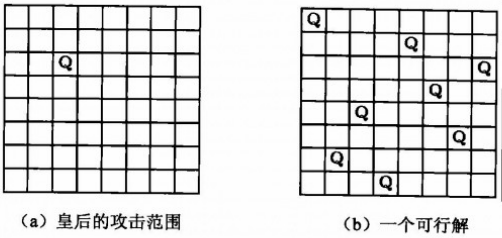
\includegraphics[width=240pt]{eight-queen.png} \\
\figcaption{八皇后问题}\label{fig:eightQueens}
\end{center}

\subsubsection{分析}
最简单的暴力枚举方法是,从64个格子中选一个子集,使得子集含有8个格子,且任意两个格子
都不在同一行、同一列或同一个对角线上。这正是子集枚举问题,然而64个格子的子集有$2^{64}$个,
太大了,这并不是一个很好的模型。

第二个思路是,从64个格子中选8个格子,这是组合生成问题。根据组合数学,有 $C_{64}^{8} \approx 4.426 \times 10^9$ 种方案,
比第一种方案优秀,但仍然不够好。

经过思考不难发现,由于每一行只能放一个皇后,那么第一行有8种选择,第二行有7中选择,…,
第8行有1中选择,总共有$8!=40320$个方案。如果用C[x]表示第x行皇后的列编号,则问题变成了一个
全排列生成问题,枚举量不会超过8!。

\subsubsection{代码}
\begin{Codex}[label=eight_queen.c]
#include <stdio.h>
#include <stdlib.h>

#define N 8 // 皇后的个数,也是棋盘的长和宽

int total = 0;  // 可行解的总数
int C[N];  // C[i]表示第i行皇后所在的列编号

/**
 * @brief 输出所有可行的棋局,按列打印.
 *
 * http://poj.grids.cn/practice/2698/ , 这题需要按列打印
 *
 * @return 无
 */
void output() {
    int i, j;
    printf("No. %d\n", total);
    for (j = 0; j < N; ++j) {
        for (i = 0; i < N; ++i) {
            if (C[i] != j) {
                printf("0 ");
            } else {
                printf("1 ");
            }
        }
        printf("\n");
    }
}

/**
 * @brief 输出所有可行的棋局,按行打印.
 * @return 无
 */
void output1() {
    int i, j;
    printf("No. %d\n", total);
    for (i = 0; i < N; ++i) {
        for (j = 0; j < N; ++j) {
            if (j != C[i]) {
                printf("0 ");
            } else {
                printf("1 ");
            }
        }
        printf("\n");
    }
}

/**
 * @brief 检查当前位置(row, column)能否放置皇后.
 *
 * @param[in] row 当前行
 * @return 能则返回1,不能则返回0
 */
int check(const int row, const int column) {
    int ok = 1;
    int i;
    for(i = 0; i < row; ++i) {
        // 两个点的坐标为(row, column), (i, C[i])
        // 检查是否在同一列,或对角线上
        if(column == C[i] || row - i == column - C[i] ||
            row - i == C[i] - column) {
            ok = 0;
            break;
        }
    }
    return ok;
}

/**
 * @brief 八皇后,深搜
 *
 * @param[in] row 搜索当前行,该在哪一列上放一个皇后
 * @return 可行解的个数
 */
int search(const int row) {
    int j;
    if (row == N) { // 终止条件,也是收敛条件,意味着找到了一个可行解
        ++total;
        output();
        return total;
    }

    for (j = 0; j < N; ++j) {  // 一列一列的试
        const int ok = check(row, j);
        if (ok) {  // 如果合法,继续递归
            C[row] = j;
            search(row + 1);
        }
    }

    return total;
}

// 表示已经放置的皇后占据了哪些列
int columns[N];
// 占据了哪些主对角线
int principal_diagonals[2 * N];
// 占据了哪些副对角线
int counter_diagonals[2 * N];

/**
 * @brief 检查当前位置(row, column)能否放置皇后.
 *
 * @param[in] row, 当前行
 * @return 能则返回1,不能则返回0
 */
int check2(const int row, const int column) {
    return columns[column] == 0 && principal_diagonals[row + column] == 0
        && counter_diagonals[row - column + N] == 0;
}

/**
 * @brief 八皇后,深搜,更优化的版本,用空间换时间
 *
 * @param[in] row 搜索当前行,该在哪一列上放一个皇后
 * @return 可行解的个数
 */
int search2(const int row) {
    int j;
    if (row == N) { // 终止条件,也是收敛条件,意味着找到了一个可行解
        ++total;
        output();
        return total;
    }

    for (j = 0; j < N; ++j) {  // 一列一列的试
        const int ok = check2(row, j);
        if (ok) {  // 如果合法,继续递归
            // 执行扩展动作
            C[row] = j;
            columns[j] = principal_diagonals[row + j] =
                    counter_diagonals[row - j + N] = 1;
            search2(row + 1);
            // 撤销动作
            C[row] = -1;  // 这句可以省略,因为C[row]会被覆盖掉
            columns[j] = principal_diagonals[row + j] =
                    counter_diagonals[row - j + N] = 0;
        }
    }

    return total;
}

int main() {
    // search(0);
    search2(0);
    return 0;
}
\end{Codex}

\subsubsection{相关的题目}
与本题相同的题目:
\begindot
\item 《算法竞赛入门经典》\footnote{刘汝佳,算法竞赛入门经典,清华大学出版社,2009} 第123页7.4.1节
\item 百练 2698 八皇后问题, \myurl{http://poj.grids.cn/practice/2698/}
\item wikioi 1295 N皇后问题, \myurl{http://www.wikioi.com/problem/1295/}
\myenddot

与本题相似的题目:
\begindot
\item POJ 1321 棋盘问题, \myurl{http://poj.org/problem?id=1321}
\myenddot


\section{还原IP地址} %%%%%%%%%%%%%%%%%%%%%%%%%%%%%%

\subsubsection{描述}
本题是 LeetCode Online Judge上的"Restore IP Addresses"。

给定一个只包含数字的字符串,还原出所有合法的IP地址。

例如:给定"25525511135",返回["255.255.11.135", "255.255.111.35"]。 (顺序无关紧要)

\subsubsection{分析}
这题很明显分为四步,有层次,因此可以尝试用回溯法解决。

\subsubsection{代码}
\begin{Codex}[label=restore_ip_adresses.cpp]
// LeetCode, Restore IP Addresses
class Solution {
public:
    vector<string> restoreIpAddresses(string s) {
        vector<string> result;
        string ip; // 存放中间结果
        dfs(s, 0, 0, ip, result);
        return result;
    }

    /**
     * @brief 解析字符串
     * @param[in] s 字符串,输入数据
     * @param[in] startIndex 从s的哪里开始
     * @param[in] step 当前步骤编号,从0开始编号,取值为0,1,2,3,4表示结束了
     * @param[out] intermediate 当前解析出来的中间结果
     * @param[out] result 存放所有可能的IP地址
     * @return 无
     */
    void dfs(string s, int start, int step, string ip,
            vector<string> &result) {
        if (s.size() - start > (4 - step) * 3)
            return;  // 非法结果,剪枝
        if (s.size() - start < (4 - step))
            return;  // 非法结果,剪枝

        if (start == s.size() && step == 4) {  // 找到一个合法解
            ip.resize(ip.size() - 1);
            result.push_back(ip);
            return;
        }

        int num = 0;
        for (int i = start; i < start + 3; i++) {
            num = num * 10 + (s[i] - '0');

            if (num <= 255) {  // 当前结点合法,则继续往下递归
                ip += s[i];
                dfs(s, i + 1, step + 1, ip + '.', result);
            }
            if (num == 0) break;  // 不允许前缀0,但允许单个0
        }
    }
};
\end{Codex}


\section{Combination Sum} %%%%%%%%%%%%%%%%%%%%%%%%%%%%%%

\subsubsection{描述}
本题是 LeetCode Online Judge上的"Combination Sum"。

给定一个数的集合(C)和一个目标数(T),找到C中所有不重复的组合,让这些被选出来的数加起来等于T。

每一个数可以被选无数次。

注意:
\begindot
\item 所有的数(包括目标)都是正整数
\item 一个组合($a_1,a_2,\cdot,a_k$)中的元素必须以非递减顺序排列
\item 一个组合不能与另一个组合重复
\myenddot

例如,给定一组数2,3,6,7,和目标7,则答案是
\begin{Code}
[7]
[2, 2, 3] 
\end{Code}

\subsubsection{分析}
这题没有固定的步骤数,但是步骤也是有限的,因此可以尝试用回溯法。

\subsubsection{代码}

\begin{Codex}[label=combination_sum.cpp]
// LeetCode, Combination Sum
class Solution {
public:
    vector<vector<int> > combinationSum(vector<int> &nums, int target) {
        sort(nums.begin(), nums.end());
        vector<vector<int> > result; // 最终结果
        vector<int> intermediate; // 中间结果
        dfs(nums, target, 0, intermediate, result);
        return result;
    }

private:
    void dfs(vector<int>& nums, int gap, int level, vector<int>& intermediate,
            vector<vector<int> > &result) {
        if (gap == 0) {  // 找到一个合法解
            result.push_back(intermediate);
            return;
        }
        for (size_t i = level; i < nums.size(); i++) { // 扩展状态
            if (gap < nums[i]) return; // 剪枝

            intermediate.push_back(nums[i]); // 执行扩展动作
            dfs(nums, gap - nums[i], i, intermediate, result);
            intermediate.pop_back();  // 撤销动作
        }
    }
};
\end{Codex}


\section{Combination Sum II} %%%%%%%%%%%%%%%%%%%%%%%%%%%%%%

\subsubsection{描述}
本题是 LeetCode Online Judge上的"Combination Sum II"。

本题与上一题唯一不同的是,每个数只能使用一次。

\subsubsection{分析}
这题没有固定的步骤数,但是步骤也是有限的,因此可以尝试用回溯法。

\subsubsection{代码}
\begin{Codex}[label=combination_sum2.cpp]
// LeetCode, Combination Sum II
class Solution {
public:
    vector<vector<int> > combinationSum2(vector<int> &nums, int target) {
        sort(nums.begin(), nums.end()); // 跟第 50 行配合,
                                             // 确保每个元素最多只用一次
        vector<vector<int> > result;
        vector<int> intermediate;
        dfs(nums, target, 0, intermediate, result);
        return result;
    }
private:
    // 使用nums[index, nums.size())之间的元素,能找到的所有可行解
    static void dfs(vector<int> &nums, int gap, int index,
            vector<int> &intermediate, vector<vector<int> > &result) {
        if (gap == 0) {  //  找到一个合法解
            result.push_back(intermediate);
            return;
        }

        int previous = -1;
        for (size_t i = index; i < nums.size(); i++) {
            // 如果上一轮循环没有选nums[i],则本次循环就不能再选nums[i],
            // 确保nums[i]最多只用一次
            if (previous == nums[i]) continue;

            if (gap < nums[i]) return;  // 剪枝

            previous = nums[i];

            intermediate.push_back(nums[i]);
            dfs(nums, gap - nums[i], i + 1, intermediate, result);
            intermediate.pop_back();  // 恢复环境
        }
    }
};
\end{Codex}


\section{小结} %%%%%%%%%%%%%%%%%%%%%%%%%%%%%%
\label{sec:dfs-template}


\subsection{适用场景}

注意,这里的总结是一种经验,一种概率,不是绝对的结论!

\textbf{输入数据}:如果是递归数据结构,如单链表,二叉树,集合,则百分之百可以用深搜;如果是非递归数据结构,如一维数组,二维数组,字符串,图,则概率小一些。

\textbf{状态转换图}:树或者图。

\textbf{求解目标}:必须要走到最深(例如对于树,必须要走到叶子节点)才能得到一个解,这种情况适合用深搜。


\subsection{思考的步骤}
\begin{enumerate}
\item 是求路径条数,还是路径本身(或动作序列)?深搜最常见的三个问题,求可行解的总数,求一个可行解,求所有可行解。
    \begin{enumerate}
    \item 如果是求路径本身,则要用一个数组\fn{path[]}存储路径。跟宽搜不同,宽搜虽然最终求的也是一条路径,但是需要存储扩展过程中的所有路径,在没找到答案之前所有路径都不能放弃;而深搜,在搜索过程中始终只有一条路径,因此用一个数组就足够了。
    \item 如果是路径条数,则不需要存储路径。
    \end{enumerate}

\item 只要求一个解,还是要求所有解?如果只要求一个解,那找到一个就可以返回;如果要求所有解,找到了一个后,还要继续扩展,直到遍历完。广搜一般只要求一个解,因而不需要考虑这个问题(广搜当然也可以求所有解,这时需要扩展到所有叶子节点,相当于在内存中存储整个状态转换图,非常占内存,因此广搜不适合解这类问题)。

\item 如何表示状态?即一个状态需要存储哪些些必要的数据,才能够完整提供如何扩展到下一步状态的所有信息。跟广搜不同,深搜的惯用写法,不是把数据记录在状态\fn{struct}里,而是添加函数参数(有时为了节省递归堆栈,用全局变量),\fn{struct}里的字段与函数参数一一对应。

\item 如何扩展状态?这一步跟上一步相关。状态里记录的数据不同,扩展方法就不同。对于固定不变的数据结构(一般题目直接给出,作为输入数据),如二叉树,图等,扩展方法很简单,直接往下一层走,对于隐式图,要先在第1步里想清楚状态所带的数据,想清楚了这点,那如何扩展就很简单了。

\item 关于判重
    \begin{enumerate}
    \item 如果状态转换图是一棵树,则不需要判重,因为在遍历过程中不可能重复。
    \item 如果状态转换图是一个图,则需要判重,方法跟广搜相同,见第 \S \ref{sec:bfs-template} 节。这里跟第8步中的加缓存是相同的,如果有重叠子问题,则需要判重,此时加缓存自然也是有效果的。
    \end{enumerate}

\item 终止条件是什么?终止条件是指到了不能扩展的末端节点。对于树,是叶子节点,对于图或隐式图,是出度为0的节点。

\item {收敛条件是什么?收敛条件是指找到了一个合法解的时刻。如果是正向深搜(父状态处理完了才进行递归,即父状态不依赖子状态,递归语句一定是在最后,尾递归),则是指是否达到目标状态;如果是逆向深搜(处理父状态时需要先知道子状态的结果,此时递归语句不在最后),则是指是否到达初始状态。

由于很多时候终止条件和收敛条件是是合二为一的,因此很多人不区分这两种条件。仔细区分这两种条件,还是很有必要的。

为了判断是否到了收敛条件,要在函数接口里用一个参数记录当前的位置(或距离目标还有多远)。如果是求一个解,直接返回这个解;如果是求所有解,要在这里收集解,即把第一步中表示路径的数组\fn{path[]}复制到解集合里。}

\item 如何加速?
    \begin{enumerate}
    \item 剪枝。深搜一定要好好考虑怎么剪枝,成本小收益大,加几行代码,就能大大加速。这里没有通用方法,只能具体问题具体分析,要充分观察,充分利用各种信息来剪枝,在中间节点提前返回。
    \item 缓存。如果子问题的解会被重复利用,可以考虑使用缓存。
        \begin{enumerate}
            \item 前提条件:子问题的解会被重复利用,即子问题之间的依赖关系是有向无环图(DAG)。如果依赖关系是树状的(例如树,单链表),没必要加缓存,因为子问题只会一层层往下,用一次就再也不会用到,加了缓存也没什么加速效果。
            \item 具体实现:可以用数组或HashMap。维度简单的,用数组;维度复杂的,用HashMap,C++有\fn{map},C++ 11以后有\fn{unordered_map},比\fn{map}快。
        \end{enumerate}
    
    \end{enumerate}
\end{enumerate}

拿到一个题目,当感觉它适合用深搜解决时,在心里面把上面8个问题默默回答一遍,代码基本上就能写出来了。对于树,不需要回答第5和第8个问题。如果读者对上面的经验总结看不懂或感觉“不实用”,很正常,因为这些经验总结是笔者做了很多深搜题后总结出来的,从思维的发展过程看,“经验总结”要晚于感性认识,所以这时候建议读者先做做后面的题目,积累一定的感性认识后,在回过头来看这一节的总结,相信会和笔者有共鸣。


\subsection{代码模板}

\begin{Codex}[label=dfs_template.cpp]
/**
 * dfs模板.
 * @param[in] input 输入数据指针
 * @param[inout] cur or gap 标记当前位置或距离目标的距离
 * @param[out] path 当前路径,也是中间结果
 * @param[out] result 存放最终结果
 * @return 路径长度,如果是求路径本身,则不需要返回长度
 */
void dfs(type *input, type *path, int cur or gap, type *result) {
    if (数据非法) return 0;   // 终止条件
    if (cur == input.size( or gap == 0)) { // 收敛条件
        将path放入result
    }

    if (可以剪枝) return;

    for(...) { // 执行所有可能的扩展动作
        执行动作,修改path
        dfs(input, step + 1 or gap--, result);
        恢复path
    }
}
\end{Codex}


\subsection{深搜与回溯法的区别}
深搜(Depth-first search, DFS)的定义见\myurl{http://en.wikipedia.org/wiki/Depth_first_search},回溯法(backtracking)的定义见\myurl{http://en.wikipedia.org/wiki/Backtracking}

\textbf{回溯法 = 深搜 + 剪枝}。一般大家用深搜时,或多或少会剪枝,因此深搜与回溯法没有什么不同,可以在它们之间画上一个等号。本书同时使用深搜和回溯法两个术语,但读者可以认为二者等价。

深搜一般用递归(recursion)来实现,这样比较简洁。

深搜能够在候选答案生成到一半时,就进行判断,抛弃不满足要求的答案,所以深搜比暴力搜索法要快。


\subsection{深搜与递归的区别}
深搜经常用递归(recursion)来实现,二者常常同时出现,导致很多人误以为他俩是一个东西。

深搜,是逻辑意义上的算法,递归,是一种物理意义上的实现,它和迭代(iteration)是对应的。深搜,可以用递归来实现,也可以用栈来实现;而递归,一般总是用来实现深搜。可以说,\textbf{递归一定是深搜,深搜不一定用递归}。

递归有两种加速策略,一种是\textbf{剪枝(prunning)},对中间结果进行判断,提前返回;一种是\textbf{加缓存}(就变成了memoization,备忘录法),缓存中间结果,防止重复计算,用空间换时间。

其实,递归+缓存,就是一种 memorization 。所谓\textbf{memorization}(翻译为备忘录法,见第 \S \ref{sec:dp-vs-memorization}节),就是"top-down with cache"(自顶向下+缓存),它是Donald Michie 在1968年创造的术语,表示一种优化技术,在top-down 形式的程序中,使用缓存来避免重复计算,从而达到加速的目的。

\textbf{memorization 不一定用递归},就像深搜不一定用递归一样,可以在迭代(iterative)中使用 memorization 。\textbf{递归也不一定用 memorization},可以用memorization来加速,但不是必须的。只有当递归使用了缓存,它才是 memorization 。

既然递归一定是深搜,为什么很多书籍都同时使用这两个术语呢?在递归味道更浓的地方,一般用递归这个术语,在深搜更浓的场景下,用深搜这个术语,读者心里要弄清楚他俩大部分时候是一回事。在单链表、二叉树等递归数据结构上,递归的味道更浓,这时用递归这个术语;在图、隐士图等数据结构上,递归的比重不大,深搜的意图更浓,这时用深搜这个术语。

\chapter{分治法}

二分查找,快速排序,归并排序,都属于分治法(Divide and Conquer)。

\section{棋盘覆盖} %%%%%%%%%%%%%%%%%%%%%%%%%%%%%%

\section{循环赛日程表} %%%%%%%%%%%%%%%%%%%%%%%%%%%%%%


\chapter{贪心法}
我们前面见过的一些算法,比如单源最短路径、最小生成树等都属于贪心法(greedy algorithm)。

如果一个问题具有以下两个要素:
\begindot
\item 最优子结构(optimal substructure)
\item 贪心选择性质(greedy-choice property)
\myenddot
则可以用贪心法求最优解。


\section{最优装载} %%%%%%%%%%%%%%%%%%%%%%%%%%%%%%


\section{哈弗曼编码} %%%%%%%%%%%%%%%%%%%%%%%%%%%%%%
\subsubsection{描述}
给定一个英文字符串,使用0和1对其进行编码,求最优前缀编码,使其所需要的比特数最少。

\subsubsection{分析}
题目很长,不过就是哈弗曼编码。

\subsubsection{代码}
\begin{Codex}[label=poj1521_entropy.cpp]
// 本题考查哈弗曼编码,但只需要统计哈弗曼编码后的总码长即可,
// 没必要建哈弗曼树得出哈弗曼编码
#include <stdio.h>
#include <string.h>
#include <queue>
#include <functional>

const int LINE_MAX = 256; // 一行最大字符数
const int MAX_ASCII = 128; // ASCII码最大值

int main_entropy() {
    char    s[LINE_MAX];
    int     count[MAX_ASCII] = {0}; // count[i]记录ASCII码为i的字符的出现次数
    int     sum;
    // 小根堆,队列头为最小元素
    std::priority_queue<int, std::vector<int>, std::greater<int> >    pq;

    while (scanf("%s", s) > 0) {
        sum = 0; // 清零
        const int len = strlen(s);

        if (strcmp(s,"END") == 0) {
            break;
        }

        for (int i = 0; i < len; i++) {
            count[s[i]]++;
        }

        for (int i = 0;i < MAX_ASCII; i++) {
            if (count[i] > 0) {
                pq.push(count[i]);
                count[i] = 0;
            }
        }
        while (pq.size() > 1) {
            const int a = pq.top(); pq.pop();
            const int b = pq.top(); pq.pop();
            sum += a + b; 
            pq.push(a + b);
        }
        if (sum == 0) {
            sum = len; // 此时pq中只有一个元素
        }
        
        while (!pq.empty()) { // clear
            pq.pop();
        }
        // 注意精度设置
        printf("%d %d %.1f\n", 8 * len, sum, ((double)8 * len) / sum);
    }
    return 0;
}
\end{Codex}

\subsubsection{类似的题目}
与本题相同的题目:
\begindot
\item POJ 1521 Entropy, \myurl{http://poj.org/problem?id=1521}
\myenddot

与本题相似的题目:
\begindot
\item  POJ 3253 Fence Repair, \myurl{http://poj.org/problem?id=3253}
\item 《算法竞赛入门经典》\footnote{刘汝佳,算法竞赛入门经典,清华大学出版社,2009} 第155页例题8-5
\item  《Introduction to Algorithms》\footnote{CLRS,Introduction to Algorithms(3rd Edition), 2009} 第16.3节
\item 《算法设计与分析(第3版)》\footnote{王晓东,计算机算法设计与分析(第3版), 2007} 第109页4.4节
\myenddot


\section{部分背包问题} %%%%%%%%%%%%%%%%%%%%%%%%%%%%%%

\chapter{动态规划}
如果一个问题具有以下两个要素:
\begindot
\item 最优子结构(optimal substructure)
\item 重叠子问题(overlap subproblem)
\myenddot
则可以用动态规划求最优解。

动态规划分为4个步骤:
\begindot
\item 描述最优解的结构。即抽象出一个状态来表示最优解。
\item 递归的定义最优解的值。找出状态转移方程,然后递归的定义
\item 计算最优解的值。典型的做法是自底向上,当然也可以自顶向下。
\item 根据计算过程中得到的信息,构造出最优解。如果我们只需要最优解的值,不需要最
优解本身,则可以忽略第4步。当执行第4步时,我们需要在第3步的过程中维护一些额外的
信息,以便我们能方便的构造出最优解。
\myenddot
在第1步中,我们需要抽象出一个“状态”,在第2步中,我们要找出“状态转移方程”,然后才能
递归的定义最优解的值。第3步和第4步就是写代码实现了。

写代码实现时有两种方式,“递归(recursive)+自顶向下(top-down)+表格(memoization)”和
“自底向上(bottom-up)+表格”。

动规用表格将各个子问题的最优解存起来,避免重复计算,是一种空间换时间。

动规与贪心的相同点:最优子结构。

不同点:1、动规的子问题是重叠的,而贪心的子问题是不重叠的(disjoint subproblems);
2、动规不具有贪心选择性质。

分治和贪心的相同点:disjoint subproblems。

\section{数字三角形} %%%%%%%%%%%%%%%%%%%%%%%%%%%%%
有一个由非负整数组成的三角形,第一行只有一个数,除了最下一行之外每个数的左下角和右下
角各有一个数,如图~~\ref{fig:numbersTriangle}所示。

\begin{center}
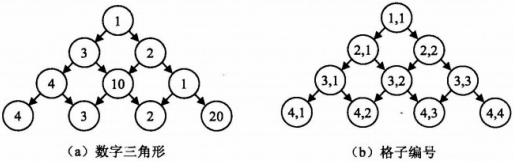
\includegraphics[width=360pt]{numbers-triangle.png}\\
\figcaption{数字三角形问题}\label{fig:numbersTriangle}
\end{center}

从第一行的数开始,每次可以往左下或右下走一格,直到走到最下行,把沿途经过的数全部加起来。
如何走才能使得这个和最大?

\textbf{Input}

Your program is to read from standard input. The first line contains one integer N: the 
number of rows in the triangle. The following N lines describe the data of the triangle. 
The number of rows in the triangle is > 1 but <= 100. The numbers in the triangle, 
all integers, are between 0 and 99.

\textbf{Output}

Your program is to write to standard output. The highest sum is written as an integer.

\textbf{Sample Input} \\
5 \\
7 \\
3 8 \\
8 1 0  \\
2 7 4 4 \\
4 5 2 6 5

\textbf{Sample Output} \\
30

\subsubsection{分析}
这是一个动态决策问题,在每层有两种选择,左下或右下,因此一个n层的数字三角形有$2^n$条路线。

可以用回溯法,用回溯法求出所有可能的路线,就可以从中选出最优路线。但是由于有$2^n$条路线,
回溯法很慢。

本题可以用动态规划来求解(具有最有子结构和重叠子问题两个要素,后面会看到)。把当前位置(i,j)看
成一个状态,然后定义状态(i,j)的指数函数d(i,j)为从位置(i,j)出发时能得到的最大和(包括格子(i,j)本
身的值a(i,j))。在这个状态定义下,原问题的解是d(1,1)。

下面来看看不同状态之间是怎样转移的。从位置(i,j)出发有两种决策,如果往左走,则走到(i+1,j)后需要求
“从(i+1,j)出发后能得到的最大和”这一子问题,即d(i+1,j),类似地,往右走之后需要求d(i+1,j+1)。应该
选择d(i+1,j)和d(i+1,j+1)中较大的一个,因此可以得到如下的状态转移方程:
$$d(i,j)=a(i,j)+\max{d(i+1,j), d(i+1,j+1)}$$

\subsubsection{代码}
版本1,自顶向下。

\begin{Codex}[label=numbers_triangle1.c]
#include<stdio.h>
#include<string.h>

#define MAXN 100

int n, a[MAXN][MAXN], d[MAXN][MAXN];

static int max(const int x, const int y) {
    return x > y ? x : y;
}

/**
 * @brief 求从位置(i,j)出发时能得到的最大和
 * @param[in] i 行
 * @param[in] j 列
 * @return 最大和
 */
static int f(const int i, const int j) {
    if(d[i][j] >= 0) {
        return d[i][j];
    } else {
        return d[i][j] = a[i][j] + (i == n-1 ? 0 : max(f(i+1, j+1), f(i+1, j)));
    }
}

int main() {
    int i, j;
    memset(d, -1, sizeof(d));

    scanf("%d", &n);
    for(i = 0; i < n; i++)
      for (j = 0; j <= i; j++) scanf("%d", &a[i][j]);
    
    printf("%d\n", f(0, 0));
    return 0;
}

\end{Codex}

版本2,自底向上。

\begin{Codex}[label=numbers_triangle2.c]
#include<stdio.h>
#include<string.h>

#define MAXN 100

int n, a[MAXN][MAXN], d[MAXN][MAXN];

static int max(const int x, const int y) {
    return x > y ? x : y;
}

/**
 * @brief 自底向上计算所有子问题的最优解
 * @return 无
 */
static void f() {
    int i, j;
    for (i = 0; i < n; ++i) {
        d[n-1][i] = a[n-1][i];
    }
    for (i = n-2; i >= 0; --i)
      for (j = 0; j <= i; ++j)
        d[i][j] = a[i][j] + max(d[i+1][j], d[i+1][j+1]);
}

int main() {
    int i, j;
    memset(d, -1, sizeof(d));

    scanf("%d", &n);
    for(i = 0; i < n; i++)
      for (j = 0; j <= i; j++) 
          scanf("%d", &a[i][j]);

    f();
    
    printf("%d\n", d[0][0]);
    return 0;
}
\end{Codex}

\subsubsection{类似的题目}
与本题相同的题目:
\begindot
\item 《算法竞赛入门经典》\footnote{刘汝佳,算法竞赛入门经典,清华大学出版社,2009}第159页9.1.1节
\item  POJ 1163 - The Triangle, \myurl{http://poj.org/problem?id=1163}
\myenddot

与本题相似的题目:
\begindot
\item  TODO
\myenddot

\section{最长公共子序列} %%%%%%%%%%%%%%%%%%%%%%%%%%%%%%

\section{0-1背包} %%%%%%%%%%%%%%%%%%%%%%%%%%%%%%
\chapter{图}
在ACM竞赛中,图一般使用邻接矩阵表示,代码框架如下;

\begin{Codex}[label=graph.c]
#define MAXN 100  // 顶点最大个数

int n; // 顶点个数
int G[MAXN][MAXN]; // 邻接矩阵
int visited_edges[MAXN][MAXN]; // 边的访问历史记录
int visited_vertices[MAXN]; // 顶点的访问历史记录
\end{Codex}

\section{深度优先搜索} %%%%%%%%%%%%%%%%%%%%%%%%%%%%%%
图的深度优先搜索的代码框架如下:

\begin{Codex}[label=graph.c]
/**
 * @brief 图的深度优先搜索代码框架,搜索边.
 * @param[in] u 出发顶点
 * @param[in] n 顶点个数
 * @param[in] G 图的临街举着
 * @param[in] visited 边的访问历史记录
 * @return 无
 * @remark 在使用的时候,为了降低递归的内存占用量,可以把
 * n, G, visited 抽出来作为全局变量
 */
void dfs(const int u, 
                const int n, const int G[][MAXN], int visited[][MAXN]) {
    int v;
    for(v = 0;  v < n; v++) if(G[u][v] && !visited[u][v]) {
        visited[u][v] = visited[v][u] = 1; // 无向图用这句
        // visited_edges[u][v] = 1; // 有向图用这句
        dfs(v, n, G, visited);
        // 这里写逻辑代码
        // printf("%d %d\n", u, v);
    }
}

/**
 * @brief 图的深度优先搜索代码框架,搜索顶点.
 * @param[in] u 出发顶点
 * @param[in] n 顶点个数
 * @param[in] G 图的临街举着
 * @param[in] visited 顶点的访问历史记录
 * @return 无
 * @remark 在使用的时候,为了降低递归的内存占用量,可以把
 * n, G, visited 抽出来作为全局变量
 */
void dfs(const int u, 
                const int n, const int G[][MAXN], int visited[MAXN]) {  
    int v;
    visited[u] = 1;
    for(v = 0;  v < n; v++) if(G[u][v] && !visited[v]) {
        dfs(v, n, G, visited);
        // 这里写逻辑代码
        // printf("%d %d\n", u, v);
    }
}
\end{Codex}

\subsection{黑白图像}

\subsubsection{描述}
输入一个n*n的黑白图像(1表示黑丝,0表示白色),任务是统计其中八连块的个数。
如果两个黑格子有公共边或者公共定点,就说它们属于同一个八连块。如图~\ref{fig:blackwhiteImage}所示的
黑白图像中有3个八连块。

\begin{center}
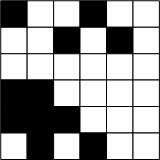
\includegraphics[width=90pt]{blackwhite-image.jpg}\\
\figcaption{拥有3个八连块的黑白图}\label{fig:blackwhiteImage}
\end{center}

\subsubsection{代码}
\begin{Codex}[label=blackwhite_image.c]
#include <stdio.h>
#include <string.h>

#define MAXN 16

int n;
// 黑白图,1 表示黑色,0表示白色,加一圈0,用于判断出界
int G[MAXN + 1][MAXN + 1];
// 记录格子(x,y)是否已经被访问过
int visitied[MAXN][MAXN];

void dfs(const int x, const int y) {
    // 曾经访问过这个格子,或者当前格子是白色
    if(G[x][y] == 0 || visitied[x][y] == 1)  return;
    
    visitied[x][y] = 1; // 标记(x,y)已访问过
    // 递归访问周围的8个格子
    dfs(x - 1, y - 1); // 左上角
    dfs(x - 1, y); // 正上方
    dfs(x - 1, y + 1); // 右上角
    dfs(x, y - 1); // 左边
    dfs(x, y + 1); // 右边
    dfs(x + 1, y - 1); // 左下角
    dfs(x + 1, y); // 正下方
    dfs(x + 1, y + 1); // 右下角
}

/*
Sample Input
6
100100
001010
000000
110000
111000
010100
Sample Output
3
*/
int main() {
    int i, j;
    char s[MAXN]; // 矩阵的一行
    int count = 0; // 八连块的个数

    scanf("%d", &n);
    memset(G, 0, sizeof(G));
    memset(visitied, 0, sizeof(visitied));

    for(i = 0; i < n; ++i) {
        scanf("%s", s);
        for(j = 0; j < n; ++j) {
            G[i + 1][j + 1] = s[j] - '0'; // 把图像往中间挪一点,空出一圈白格子
        }
    }


    for(i = 1; i <= n; ++i) {
        for(j = 1; j <= n; ++j) {
            if(visitied[i][j] == 0 && G[i][j] == 1) {
                count++;
                dfs(i, j);
            }
        }
    }
    printf("%d\n", count);
    return 0;
}
\end{Codex}

\subsubsection{相关的题目}
与本题相同的题目:
\begindot
\item 《算法竞赛入门经典》\footnote{刘汝佳,算法竞赛入门经典,清华大学出版社,2009} 第107页6.4.1节
\item  None
\myenddot

与本题相似的题目:
\begindot
\item  None
\myenddot

\subsection{欧拉回路}

\subsubsection{描述}
本题是 UVA 10054 - The Necklace。

My little sister had a beautiful necklace made of colorful beads. Two successive beads in the 
necklace shared a common color at their meeting point. The figure below shows a segment of 
the necklace:

\centerline{\fbox{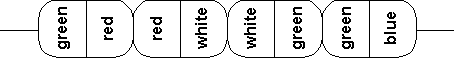
\includegraphics[width=240pt]{uva10054.png}}}

But, alas! One day, the necklace was torn and the beads were all scattered over the floor. 
My sister did her best to recollect all the beads from the floor, but she is not sure 
whether she was able to collect all of them. Now, she has come to me for help. She wants
 to know whether it is possible to make a necklace using all the beads she has in the same
 way her original necklace was made and if so in which order the bids must be put.

Please help me write a program to solve the problem.

\subsubsection{Input}
The input contains T test cases. The first line of the input contains the integer T.

The first line of each test case contains an integer $N(5 \leq N \leq 1000)$ giving the number of beads 
my sister was able to collect. Each of the next N lines contains two integers describing 
the colors of a bead. Colors are represented by integers ranging from 1 to 50.

\subsubsection{Output}
For each test case in the input first output the test case number as shown in the sample output. Then 
if you apprehend that some beads may be lost just print the sentence ``some beads may be lost" on a 
line by itself. Otherwise, print N lines with a single bead description on each line. Each bead 
description consists of two integers giving the colors of its two ends. For $1 \leq i \leq N_1$, the second integer 
on line i must be the same as the first integer on line i + 1. Additionally, the second integer 
on line N must be equal to the first integer on line 1. Since there are many solutions, any one
 of them is acceptable.

Print a blank line between two successive test cases.

\subsubsection{Sample Input}
\begin{Code}
2
5
1 2
2 3
3 4
4 5
5 6
5
2 1
2 2
3 4
3 1
2 4
\end{Code}

\subsubsection{Sample Output}
\begin{Code}
Case #1
some beads may be lost

Case #2
2 1
1 3
3 4
4 2
2 2
\end{Code}

\subsubsection{分析}
这题就是欧拉回路+打印路径。

如果能从图的某一顶点出发,每条边恰好经过一次,这样的路线称为\textbf{欧拉道路}(Eulerian Path)。
如果每条边恰好经过一次,且能回到起点,这样的路线称为\textbf{欧拉回路}(Eulerian Circuit)。

对于无向图G,当且仅当G是连通的,且最多有两个奇点,则存在欧拉道路。
如果有两个奇点,则必须从其中一个奇点出发,到另一个奇点终止。

如果没有奇点,则一定存在一条欧拉回路。

对于有向图G,当且仅当G是连通的,且每个点的入度等于出度,则存在欧拉回路。

如果有两个顶点的入度与出度不相等,且一个顶点的入度比出度小1,另一个顶点的入度比出度大1,此时,
存在一条欧拉道路,以前一个顶点为起点,以后一个顶点为终点

\subsubsection{代码}
\begin{Codex}[label=eulerian_circuit.c]
#include <stdio.h>
#include<string.h>

#define MAXN 51  // 顶点最大个数

int G[MAXN][MAXN];
int visited_vertices[MAXN]; 
int visited_edges[MAXN][MAXN];
int count[MAXN]; // 顶点的度

void dfs(const int u) {  
    int v;
    visited_vertices[u] = 1;
    for(v = 0;  v < MAXN; v++) if(G[u][v] && !visited_vertices[v]) {
        dfs(v);
    }
}

/*
 * @brief 欧拉回路,允许自环和重复边
 * @param[in] u 起点
 * @return 无
 */
void euler(const int u){
    int v;
    for(v = 0; v < MAXN; ++v) if(G[u][v]){
        --G[u][v]; --G[v][u]; // 这个技巧,即有visited的功能,又允许重复边
        euler(v);
        // 逆向打印,或者存到栈里再打印
        printf("%d %d\n", u, v);
    }
}

int main() {
    int T, N, a, b;
    int i;
    int cases=1;
    scanf("%d",&T);
    while(T--) {
        int flag = 1; // 结点的度是否为偶数
        int flag2 = 1; // 图是否是连通的
        
        memset(G, 0, sizeof(G));
        memset(count, 0, sizeof(count));

        scanf("%d",&N);
        for(i = 0; i < N; ++i){
            scanf("%d %d", &a, &b); 
            ++G[a][b];
            ++G[b][a];
            ++count[a];
            ++count[b];
        }

        printf("Case #%d\n", cases++);

        // 欧拉回路形成的条件之一,判断结点的度是否为偶数
        for(i=0; i<MAXN; ++i) {
            if(count[i] & 1){
                flag = 0;
                break;
            }
        }
        // 检查图是否连通
        if(flag) {
            memset(visited_vertices, 0, sizeof(visited_vertices));
            memset(visited_edges, 0, sizeof(visited_edges));

            for(i=0; i< MAXN; ++i) 
                if(count[i]) { 
                    dfs(i);
                    break; 
                }
            for(i=0; i< MAXN; ++i){
                if(count[i] && !visited_vertices[i]) {
                    flag2 = 0; 
                    break;
                }
            }
        }
        if (flag && flag2) {
            for(i = 0; i < MAXN; ++i) if(count[i]){
                euler(i);
                break;
            }
        } else {
            printf("some beads may be lost\n");
        }

        if(T > 0) printf("\n");
    }
    return 0;
}
\end{Codex}

\subsubsection{相关的题目}
与本题相同的题目:
\begindot
\item 《算法竞赛入门经典》\footnote{刘汝佳,算法竞赛入门经典,清华大学出版社,2009} 第111页6.4.4节
\item  None
\myenddot

与本题相似的题目:
\begindot
\item  UVa 10129 Play on Words, \myurl{http://t.cn/zTInBDX}
\myenddot


\section{广度优先搜索} %%%%%%%%%%%%%%%%%%%%%%%%%%%%%%



\section{最小生成树} %%%%%%%%%%%%%%%%%%%%%%%%%%%%%%
“最小”指的是边的权值之和最小。

构造最小生成树(Minimum Spanning Tree, MST)有多种算法。其中多数算法利用了最小生成树的一个性质(简称为MST性质):假设$N=(V, E)$是一个连通网,$U$是顶点集$V$的一个非空子集。若$(u, v)$是一条具有最小权值的边,其中$u \in U, v \in V-U$,则必存在一颗包含边$(u, v)$的最小生成树。

Prim算法和Kruskal算法是两个利用MST性质构造最小生成树的算法。它们都属于贪心法。

\subsection{Prim算法}
假设$N=(V, E)$是一个连通网,$TE$是$N$上最小生成树中边的集合。算法从$U={u_0}(u_0 \in V), TE=\{\}$开始,重复执行下述操作:在所有$u \in U, v \in V-U$的边$(u, v) \in E$中找一条代价最小的边$(u_0, v_0)$并入集合$TE$,同时$v_0$并入U,直至$U=V$为止。此时$TE$中必有$n-1$条边,则$T=(V, TE)$为$N$的最小生成树。
为实现这个算法需附设一个数组\fn{closedge},以记录从$U$到$V-U$具有最小代价的边。对每个顶点$v_i \in V-U$,在辅助数组中存在一个相应分量\fn{closedge[i-1]},它包括两个域,其中\fn{lowcost}存储该边上的权。显然,$closedge[i].lowcost=\min\left\{cost(u, v_i), u \in U\right\}$。\fn{adjvex}域存储该边依附的在U中的顶点。

图 \ref{fig:prim}所示为按Prim算法构造网的一棵最小生成树的过程,在构造过程中辅助数组中各分量值的变化如表\ref{tab:prim}所示。

\begin{center}
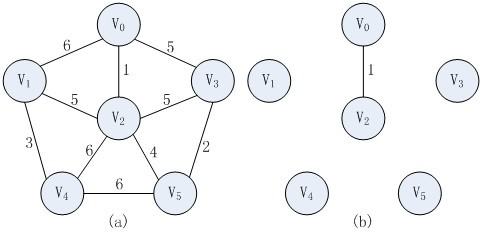
\includegraphics[width=240pt]{prim1.png}\\
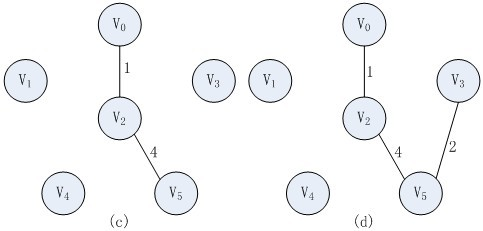
\includegraphics[width=240pt]{prim2.png}\\
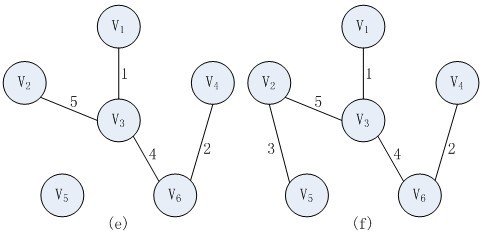
\includegraphics[width=240pt]{prim3.png}\\
\figcaption{Prim算法构造最小生成树的过程}\label{fig:prim}
\end{center}

\begin{center}
\tabcaption{构造最小生成树过程中辅助数组的变化}
\label{tab:prim}
\begin{tabular}{|c|cccccccc|}
\hline
\textbf{\diagbox{closedge}{i}} & \textbf{1} & \textbf{2} & \textbf{3} & \textbf{4}& \textbf{5}& \textbf{U}& \textbf{U-V}& \textbf{k}\\
\hline
adjvex & $v_0$ & $v_0$ & $v_0$ & & & $v_0$ & $\{v_1,v_2,v_3,v_4,v_5\}$ & \multirow{2}{*}{2} \\
lowcost & 6 & 1 & 5 & & & & & \\
\hline
adjvex & $v_2$ & & $v_1$ & $v_2$ & $v_2$ & $\{v_0,v_2\}$ & $\{v_1,v_3,v_4,v_5\}$ & \multirow{2}{*}{5} \\
lowcost & 5 & 0 & 5 & 6 & 4 & & & \\
\hline
adjvex & $v_2$ & & $v_6$ & $v_2$ & & $\{v_0,v_2,v_5\}$ & $\{v_1,v_3,v_4\}$ & \multirow{2}{*}{3} \\
lowcost & 5 & 0 & 2 & 6 & 0 & & & \\
\hline
adjvex & $v_2$ & & & $v_2$ & & $\{v_0,v_2,v_5,v_3\}$ & $\{v_1,v_4\}$ & \multirow{2}{*}{1} \\
lowcost & 5 & 0 & 0 & 6 & 0 & & & \\
\hline
adjvex & & & & $v_1$ & & $\{v_0,v_2,v_5,v_3,v_1\}$ & $\{v_4\}$ & \multirow{2}{*}{4} \\
lowcost & 0 & 0 & 0 & 3 & 0 & & & \\
\hline
adjvex & & & & & & $\{v_0,v_2,v_5,v_3,v_1,v_4\}$ & $\{\}$ & \multirow{2}{*}{} \\
lowcost & 0 & 0 & 0 & 0 & 0 & & & \\
\hline
\end{tabular}
\end{center}


\subsubsection{代码}

\begin{Codex}[label=mgraph_prim1.c]
#include <stdio.h>
#include <stdlib.h>  /* for malloc() */
#include <limits.h>  /* for INT_MAX */

/** 顶点数的最大值*/
#define MAX_VERTICES_NUM 100
/** 边的权值,对无权图,用0或1表示是否相邻;对有权图,则为权值. */
typedef int graph_weight_t;
#define GRAPH_INF INT_MAX

/**
 *@struct
 *@brief 邻接矩阵.
 */
typedef struct mgraph_t {
    int nv; /* 顶点数*/
    int ne; /* 边数*/
    /* 邻接矩阵,存放边的信息,如权重等*/
    graph_weight_t matrix[MAX_VERTICES_NUM][MAX_VERTICES_NUM];
} mgraph_t;

mgraph_t g;

typedef struct closedge_t {
    int adjvex; /* 弧头,属于U */
    /* 边 adjvex->本下标 的权值,-GRAPH_INF表示已经加入U */
    graph_weight_t lowcost;
} closedge_t;

/*
 * @brief 在V-E集合中寻找最小的边
 * @param[in] closedge MST中的边,起点为adjvex,终点为本下标
 * @param[in] n closedge数组的长度
 * @return 找到了则返回弧尾的下标,V-U为空集则返回-1,表示终止
 */
static int min_element(const closedge_t closedge[], int n) {
    int i;
    int min_value = GRAPH_INF;
    int min_loc = -1;
    for (i = 0; i < n; i++)
        if (closedge[i].lowcost > -GRAPH_INF) {
            if (min_value > closedge[i].lowcost) {
                min_value = closedge[i].lowcost;
                min_loc = i;
            }
        }
    return min_loc;
}

/**
 * @brief Prim算法,求图的最小生成树.
 * @param[in] g 图对象的指针
 * @return MST的边的权值之和
 */
graph_weight_t mgraph_prim(const mgraph_t *g) {
    graph_weight_t sum = 0; /* 权值之和 */
    int i, j;
    int u = 0; /* 从0号顶点出发 */
    const int n = g->nv;
    /* closedge[n],记录从顶点集U到V-U的边*/
    closedge_t* const closedge = (closedge_t*) malloc(n * sizeof(closedge_t));

    /* 辅助数组初始化*/
    for (i = 0; i < n; i++) if (i != u) {
        closedge[i].adjvex = u;
        closedge[i].lowcost = g->matrix[u][i];
    }
    closedge[u].lowcost = -GRAPH_INF; /* 初始, U={u} */

    for (i = 0; i < n; i++) if (i != u) { /* 其余的n-1个顶点*/
        /* 求出TE的下一个顶点k */
        const int k = min_element(closedge, n);
        /* 输出此边 closedge[k].adjvex --> k */
        printf("%c - %c : %d\n", 'A' + closedge[k].adjvex, 'A' + k,
                g->matrix[closedge[k].adjvex][k]);
        sum += g->matrix[closedge[k].adjvex][k];
        // sum += closedge[k].lowcost;  // 等价
        closedge[k].lowcost = -GRAPH_INF;  /* 顶点k并入U,表示此边加入TE */
        /* 更新k的邻接点的值,不相邻为无穷大*/
        for (j = 0; j < n; j++) {
            const graph_weight_t w = g->matrix[k][j];
            if (w < closedge[j].lowcost) {
                closedge[j].adjvex = k;
                closedge[j].lowcost = w;
            }
        }
    }
    free(closedge);
    return sum;
}

/** 读取输入,构建图. */
void read_graph() {
    int i, j, k, m, n;

    /* 读取节点和边的数目 */
    scanf("%d%d", &m, &n);
    getchar(); // 消耗回车键
    g.nv = m;
    g.ne = n;

    /* 初始化图,所有节点间距离为无穷大 */
    for (i = 0; i < m; i++) {
        for (j = 0; j < m; j++) {
            g.matrix[i][j] = GRAPH_INF;
        }
    }

    /* 读取边信息 */
    for (k = 0; k < n; k++) {
        char chx, chy;
        int w;
        scanf("%c %c %d", &chx, &chy, &w);
        getchar();
        i = chx - 'A';
        j = chy - 'A';
        g.matrix[i][j] = w;
        g.matrix[j][i] = w;
    }
}

/* test

输入数据:

7 11
A B 7
A D 5
B C 8
B D 9
B E 7
C E 5
D E 15
D F 6
E F 8
E G 9
F G 11

输出:

A - D : 5
D - F : 6
A - B : 7
B - E : 7
E - C : 5
E - G : 9
Total:39
*/
int main() {
    read_graph();
    /* 求解最小生成树 */
    printf("Total:%d\n", mgraph_prim(&g));
    return 0;
}
\end{Codex}

\subsubsection{算法分析}
假设网中有$n$个顶点,则第一个进行初始化的循环语句的频度为$n$,第二个循环语句的频度为$n-1$。其中有两个内循环:其一是在\fn{closedge[v].lowcost}中求最小值,其频度为$n-1$;其二是重新选择具有最小代价的边,其频度为$n$。因此Prim算法的时间复杂度为$O(n^2)$,与网中边数无关,因此适用于求边稠密的图的最小生成树。

Prim算法的另一种实现是使用小根堆,其流程是:小根堆中存储一个端点在生成树中,另一个端点不在生成树的边,每次从小根堆的堆顶可选出权值最小的边$(u, v)$,将其从堆中推出,加入生成树中。然后将新出现的所有一个端点在生成树中,一个端点不在生成树的边都插入小根堆中。下一轮迭代中,下一条满足要求的边又上升到堆顶。如此重复$n-1$次,最后建立起该图的最小生成树。该算法的C代码实现如下。

\subsubsection{代码}

\begin{Codex}[label=mgraph_prim2.c]
#include <stdio.h>
#include <stdlib.h>  /* for malloc() */
#include <limits.h>  /* for INT_MAX */

/** 顶点数的最大值*/
#define MAX_VERTICES_NUM 100
/** 边的权值,对无权图,用0或1表示是否相邻;对有权图,则为权值. */
typedef int graph_weight_t;
#define GRAPH_INF INT_MAX

/**
 *@struct
 *@brief 邻接矩阵.
 */
typedef struct mgraph_t {
    int nv; /* 顶点数*/
    int ne; /* 边数*/
    /* 邻接矩阵,存放边的信息,如权重等*/
    graph_weight_t matrix[MAX_VERTICES_NUM][MAX_VERTICES_NUM];
} mgraph_t;

mgraph_t g;


/**
 * @struct 边
 */
typedef struct edge_t{
    int tail;  /** 弧尾, from */
    int head;  /** 弧头, to */
    graph_weight_t w;  /** 权值 */
}edge_t;

static int edge_cmp(const edge_t *e1, const edge_t *e2) {
    return e1->w - e2->w;
}

typedef edge_t heap_elem_t; // 元素的类型

/* 等价于复制粘贴,这里为了节约篇幅,使用include,在OJ上提交时请用复制粘贴 */
#include "heap.c"  /* 见“树->堆”这节 */

/**
  * @brief Prim算法,求图的最小生成树.
  * @param[in] g 图对象的指针
  * @return MST的边的权值之和
  */
int mgraph_prim(const mgraph_t *g){
    graph_weight_t sum = 0; /* 权值之和 */
    int u = 0; /* 从0号顶点出发 */
    int i, count = 1;
    edge_t e;
    heap_t *h = heap_create(g->ne, edge_cmp);
    const int n = g->nv;
    /* 判断顶点是否已经加入最小生成树*/
    int* U = (int *)malloc(n * sizeof(int));
    for(i = 0; i < n; i++) U[i] = 0;

    /* 开始顶点加入U(所以count初始为1) */
    U[u] = 1;
    while (count < n) {
        int v;
        for(v = 0; v < n; v++) if(!U[v]) { /* 若v不在生成树,(u,v)加入堆*/
            e.tail = u;
            e.head = v;
            /* tail在树内,head不在树内*/
            e.w = g->matrix[u][v];
            heap_push(h, e);
        }
        while(!heap_empty(h) && count < n) {
            /* 从堆中退出最小权值边,存入ed */
            e = heap_top(h); heap_pop(h);
            if(!U[e.head]) {
                /* 输出生成树TE的边,即此边加入TE */
                printf("%c - %c: %d\n", 'A' + e.tail, 'A' + e.head,
                        g->matrix[e.tail][e.head]);
                sum += g->matrix[e.tail][e.head];
                u = e.head;
                /* u并入到生成树的顶点集合U */
                U[u] = 1;
                count++;
                break;
            }
        }
    }

    free(U);
    heap_destroy(h);
    return sum;
}

// ...
\end{Codex}

\subsubsection{算法分析}
该算法迭代次数为$O(n)$,每次迭代将平均$e/n$条边插入最小堆中,$e$条边从堆中删除,堆的插入和删除操作时间复杂度均为$O(\log_2 e)$,则总的时间复杂度为 $O(e\log_2e)$。

\subsection{Kruskal算法}
\label{sec:kruskal}
假设连通网$N={V, E}$,则令最小生成树的初始状态为只有$n$个顶点而无边的非连通图$T=(V, {})$,图中每个顶点自成一个连通分量。在$E$中选择代价最小的边,若该边依附的顶点落在$T$中不同的连通分量上,则将此边加入到$T$中,否则舍去此边而选择下一条代价最小的边。依次类推,直至T中所有顶点都在同一连通分量上为止。

图\ref{fig:kruskal}所示为Kruskal算法构造一棵最小生成树的过程。

\begin{center}
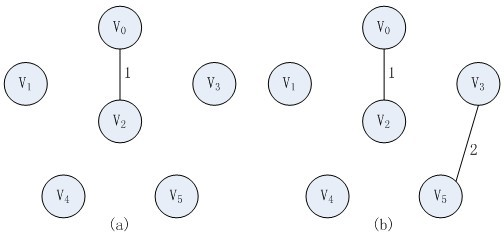
\includegraphics[width=240pt]{kruskal1.png}\\
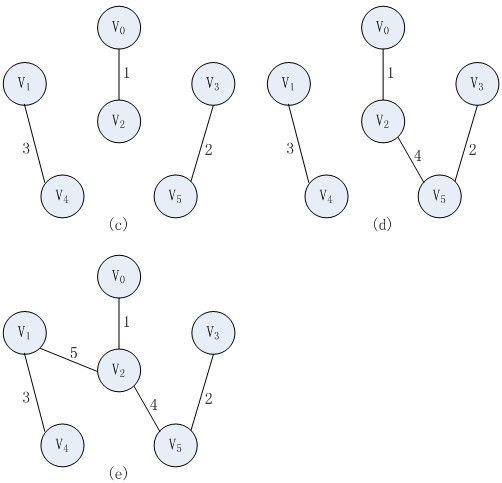
\includegraphics[width=240pt]{kruskal2.png}\\
\figcaption{Kruskal算法构造最小生成树的过程}\label{fig:kruskal}
\end{center}

下面是Kruskal算法的C语言实现。

\subsubsection{代码}

\begin{Codex}[label=kruskal.c]
#include <stdio.h>
#include <stdlib.h>  /* for malloc() */
#include <limits.h>  /* for INT_MAX */

/* 等价于复制粘贴,这里为了节约篇幅,使用include,在OJ上提交时请用复制粘贴 */
#include "ufs.c"  /* 见“树->并查集”这节 */

#define MAX_VERTICES_NO 11 /* 顶点编号最大值 */
#define MAX_EDGES 100  /* 最大边数 */
/** 边的权值,对无权图,用0或1表示是否相邻;对有权图,则为权值. */
typedef int graph_weight_t;

/**
 * @struct 无向图的边.
 */
typedef struct edge_t{
    int u;  /** 顶点编号 */
    int v;  /** 顶点编号 */
    graph_weight_t w;  /** 权值 */
} edge_t;

edge_t edges[MAX_EDGES];

static int edge_cmp(const edge_t *e1, const edge_t *e2) {
    return e1->w - e2->w;
}

typedef edge_t heap_elem_t; // 元素的类型

/* 等价于复制粘贴,这里为了节约篇幅,使用include,在OJ上提交时请用复制粘贴 */
#include "heap.c"  /* 见“树->堆”这节 */

/*
  * @brief Kruskal算法,求图的最小生成树.
  * @param[in] edges 边的数组
  * @param[in] n 边数,一定要大于或等于(顶点数-1)
  * @param[in] m 顶点数
  * @return MST的边的权值之和
  */
graph_weight_t kruskal(const edge_t edges[], int n, int m) {
    int i;
    graph_weight_t sum = 0;
    heap_t *h = heap_create(n, edge_cmp);
    ufs_t *s = ufs_create(MAX_VERTICES_NO);  /* 并查集,0位置未用  */
    if (n < m - 1) return -1;

    /* 把所有边插入堆中*/
    for (i = 0; i < n; i++) {
        heap_push(h, edges[i]);
    }

    for (i = 0; i < n; i++) {
        /* 从堆中退出最小权值边 */
        const edge_t e = heap_top(h);
        int u, v;
        heap_pop(h);
        /* 取两顶点所在集合的根*/
        u = ufs_find(s, e.u);
        v = ufs_find(s, e.v);
        if (u != v) { /* 不是同一集合,说明不连通*/
            ufs_union(s, u, v); /* 合并,连通成一个分量*/
            /* 输出生成树TE的边,即此边加入TE */
            printf("%d - %d\n", e.u, e.v);
            sum += e.w;
        }
    }

    heap_destroy(h);
    ufs_destroy(s);
    return sum;
}

static int edge_cmp1(const void *e1, const void *e2) {
    const edge_t* const ee1 = (const edge_t *)e1;
    const edge_t* const ee2 = (const edge_t *)e2;
    return ee1->w - ee2->w;
}

/** Kruskal算法,快排+并查集. */
graph_weight_t kruskal1(edge_t edges[], int n, int m) {
    int i;
    graph_weight_t sum = 0;
    ufs_t *s = ufs_create(MAX_VERTICES_NO);  /* 并查集,0位置未用  */
    if (n < m - 1) return -1;

    qsort(edges, n, sizeof(edge_t), edge_cmp1);

    for (i = 0; i < n; i++) {
        /* 从堆中退出最小权值边,存入ed */
        const edge_t e = edges[i];
        /* 取两顶点所在集合的根*/
        const int u = ufs_find(s, e.u);
        const int v = ufs_find(s, e.v);
        if (u != v) { /* 不是同一集合,说明不连通*/
            ufs_union(s, u, v); /* 合并,连通成一个分量*/
            /* 输出生成树TE的边,即此边加入TE */
            printf("%d - %d\n", e.u, e.v);
            sum += e.w;
        }
    }
    ufs_destroy(s);
    return sum;
}

/* test
输入数据:
7 11
0 1 7
0 3 5
1 2 8
1 3 9
1 4 7
2 4 5
3 4 15
3 5 6
4 5 8
4 6 9
5 6 11

输出:
0 - 3
2 - 4
3 - 5
0 - 1
1 - 4
4 - 6
Total:39
*/
int main() {
    int i, m, n;

    /* 读取顶点数,边数目*/
    scanf("%d%d", &m, &n);

    /* 读取边信息 */
    for (i = 0; i < n; i++) {
        scanf("%d %d %d", &edges[i].u, &edges[i].v, &edges[i].w);
    }

    /* 求解最小生成树 */
    printf("Total:%d\n", kruskal(edges, n, m));
    return 0;
}
\end{Codex}

\subsubsection{算法分析}
如果采用邻接矩阵作为图的存储结构,则在建立小根堆时需要检测图的邻接矩阵,这需要$O(n^2)$的时间。此外,需要将$e$条边组成初始的小根堆。如果直接从空堆开始,依次插入各边,需要$O(e\log_2e)$的时间。在构造最小生成树的过程中,需要进行$O(e)$次出堆操作\fn{heap_remove()}、$2e$次并查集的\fn{ufs_find()}操作以及$n-1$次\fn{ufs_union()}操作,计算时间分别为$O(e\log_2e)$、$O(\log_2n)$和$O(n)$,所以总时间为$O(n^2+e\log_2e)$。

如果采用邻接表作为图的存储结构,则在建立小根堆时需要检测图的邻接表,这需要$O(n+e)$的时间。为建成初始的小根堆,需要$O(e\log_2e)$的时间。在构造最小生成树的过程中,需要进行$O(e)$次出堆操作\fn{heap_remove()}、$2e$次并查集的\fn{ufs_find()}操作以及$n-1$次\fn{ufs_union()}操作,计算时间分别为$O(e\log_2e)$、$O(e\log_2n)$和$O(n)$,所以总时间为$O(n+e\log_2e)$。


\subsection{Highways}
\subsubsection{描述}
一个名叫Flatopia的岛国地势非常平坦。不幸的是Flatopia的公共高速公路系统很差劲。Flatopia的政府也意识到了这个问题,已经建造了许多高速公路用来连接比较重要的城镇。不过,仍然有一些城镇没有接入高速公路。因此,很有必要建造更多的高速公路,让任意两个城镇之间可以通过高速公路连接。

Flatopia的城镇从1到$N$编号,城镇i的位置由笛卡尔坐标$(x_i,y_i)$表示。每条高速公路仅连接两个城镇。所有的高速公路都是直线,因此它们的长度就等于两个城镇之间的欧氏距离。所有的高速公路是双向的,高速公路之间可以相交,但是司机只能在公路的端点(也即城镇)换道。

Flatopia政府希望能最小化建造高速公路的代价。由于Flatopia地势平坦,一条高速公路的代价正比于它的长度。因此,应该让高速公路的总长度最小。

\subsubsection{输入}
输入由两部分组成。第一部分描述所有的城镇,第二部分描述所有已经建造好的高速公路。

第一行包含一个整数$N(1 \leq N \leq 750)$,表示城镇的数目。接下来的$N$行每行包含一对整数,$x_i$和$y_i$,由空格隔开,表示第$i$个城镇的坐标。坐标的绝对值不会超过10000。每个城镇的坐标都不重叠。

接下来一行包含一个整数$M(0 \leq M \leq 1000)$,表示已经存在的高速公路的数目。接下来的$M$行每行包含一对整数,给出了一对城镇编号,表示这两个城镇被一条高速公路连接起来。每两个城镇之间最多被一条高速公路连接。

\subsubsection{输出}
输出所有需要新建的高速公路。每行一个高速公路,用一对城镇编号表示。

如果不需要新建高速公路,输出为空。

\subsubsection{样例输入}
\begin{Code}
9
1 5
0 0 
3 2
4 5
5 1
0 4
5 2
1 2
5 3
3
1 3
9 7
1 2
\end{Code}

\subsubsection{样例输出}
\begin{Code}
1 6
3 7
4 9
5 7
8 3
\end{Code}

\subsubsection{分析}
很明显,最小生成树。

题中的网络是一个完全图,任意两个城镇之间都有边,权值是两点间的距离。因此Prim算法比Kruskal算法效率更高。

对于已经存在的高速公路,令它们权值为0,可以保证它们一定会被选中。

因为题目只需要输出新建的高速公路的两个端点,不需要输出最小生成树的长度,所以计算距离的时候不用sqrt,也就不用double了。

\subsubsection{代码}
\begin{Codex}[label=poj_1751_highways_prim.c]
/* POJ 1751 Highways, http://poj.org/problem?id=1751 */

/* 等价于复制粘贴,这里为了节约篇幅,使用include,在OJ上提交时请用复制粘贴 */
#include "mgraph_prim1.c"  /* 见“图->最小生成树->Prim算法”这节 */

// 1. 修改范围
#define MAX_VERTICES_NUM 750
// 2. 重写 read_graph()
// 3. 重写 main()
// 4. 修改 mgraph_prim()里的printf,权值大于0才打印出来
if (g->matrix[closedge[k].adjvex][k] > 0)
    printf("%d %d\n", closedge[k].adjvex+1,  k+1);

/* 输入数据 */
int n, m, x[MAX_VERTICES_NUM], y[MAX_VERTICES_NUM];

/*
 * @brief 两点之间的距离.
 *
 * 因为题目只需要输出新建的高速公路的两个端点,不需要输出最小生成
 * 树的长度,所以计算距离的时候不用sqrt,也就不用double了。
 *
 * @param[in] i 编号为i+1的城镇
 * @param[in] j 编号为j+1的城镇
 *
 * @return 欧氏距离的平方
 */
static int distance(int i,int j) {
    return (x[i]-x[j]) * (x[i]-x[j]) + (y[i]-y[j]) * (y[i]-y[j]);
}

/** 读取输入,构建图. */
void read_graph() {
    int i, j;
    scanf("%d", &n);
    g.nv = n;
    g.ne = n * (n - 1) / 2;

    for (i = 0; i < n; i++)
        scanf("%d %d", &x[i], &y[i]);
    for (i = 0; i < n; i++)
        for (j = i; j < n; j++)
            g.matrix[i][j] = g.matrix[j][i] = distance(i, j);

    scanf("%d", &m);
    for (i = 0; i < m; i++) {
        int a, b;
        scanf("%d %d", &a, &b);
        g.matrix[a - 1][b - 1] = g.matrix[b - 1][a - 1] = 0;
    }
}

int main() {
    read_graph();
    mgraph_prim(&g);
    return 0;
}
\end{Codex}

\subsubsection{相关的题目}
与本题相同的题目:
\begindot
\item POJ 1751 Highways, \myurl{http://poj.org/problem?id=1751}
\myenddot

与本题相似的题目:
\begindot
\item POJ 2485 Highways, \myurl{http://poj.org/problem?id=2485}
\item POJ 1861 Network, \myurl{http://poj.org/problem?id=1861}
\item POJ 2395 Out of Hay, \myurl{http://poj.org/problem?id=2395}
\item POJ 2377 Bad Cowtractors, \myurl{http://poj.org/problem?id=2377}
\item POJ 2421 Constructing Roads, \myurl{http://poj.org/problem?id=2421}
\item POJ 1679 The Unique MST, \myurl{http://poj.org/problem?id=1679}
\item POJ 1258 Agri-Net, \myurl{http://poj.org/problem?id=1258}
\item POJ 1251 Jungle Roads, \myurl{http://poj.org/problem?id=1251}
\item POJ 3625 Building Roads, \myurl{http://poj.org/problem?id=3625}
\item POJ 1789 Truck History, \myurl{http://poj.org/problem?id=1789}
\myenddot


\subsection{最优布线问题 }
\subsubsection{描述}
学校需要将n台计算机连接起来,不同的2台计算机之间的连接费用可能是不同的。为了节省费用,我们考虑采用间接数据传输结束,就是一台计算机可以间接地通过其他计算机实现和另外一台计算机连接。

为了使得任意两台计算机之间都是连通的(不管是直接还是间接的),需要在若干台计算机之间用网线直接连接,现在想使得总的连接费用最省,让你编程计算这个最小的费用。

\subsubsection{输入}
输入第一行为两个整数$n,m(2 \leq n \leq 100000,2\leq m \leq 100000)$,表示计算机总数,和可以互相建立连接的连接个数。接下来$m$行,每行三个整数$a,b,c$ 表示在机器$a$和机器$b$之间建立连接的话费是$c$。(题目保证一定存在可行的连通方案, 数据中可能存在权值不一样的重边,但是保证没有自环)

\subsubsection{输出}
输出只有一行一个整数,表示最省的总连接费用。

\subsubsection{样例输入}
\begin{Code}
3 3
1 2 1
1 3 2
2 3 1
\end{Code}

\subsubsection{样例输出}
\begin{Code}
2
\end{Code}

\subsubsection{分析}
本题是非常直白的kruskal算法,可以直接使用第 \S \ref{sec:kruskal}节的样例代码。

\subsubsection{代码}
\begin{Codex}[label=wiring.c]
/* wikioi 1231 最优布线问题, http://www.wikioi.com/problem/1231/ */
// 1. 修改范围
#define MAX_VERTICES_NO 100001 /* 顶点编号最大值 */
#define MAX_EDGES 100000  /* 最大边数 */
// 2. 注释掉 kruskal()里的printf()
// 3. sum类型改为 long long,kruskal()返回值改为 long long
// 4. main()里的printf改为 %lld

/* 等价于复制粘贴,这里为了节约篇幅,使用include,在OJ上提交时请用复制粘贴 */
#include "kruskal.c"  /* 见“图->最小生成树->Kruskal算法”这节 */
\end{Codex}

\subsubsection{相关的题目}
与本题相同的题目:
\begindot
\item wikioi 1231 最优布线问题, \myurl{http://www.wikioi.com/problem/1231/}
\myenddot

与本题相似的题目:
\begindot
\item None
\myenddot


\section{最短路径} %%%%%%%%%%%%%%%%%%%%%%%%%%%%%%

\subsection{单源最短路径——Dijkstra算法}
\label{sec:dijkstra}

假设$S$为已求得最短路径的点的集合,则可证明:下一条最短路径(设其终点为$x$)或者是弧$(v, x)$,或者是中间只经过$S$中的顶点而最后到达顶点$x$的路径。

Dijkstra算法流程如下:
\begin{enumerate}
\item $S$为已找到从$v$出发的最短路径的终点的集合,它的初始状态为空集。\fn{dist[i]}存放的是$v$到$v_i$的最短路径长度,根据前面所述性质,\fn{dist[i]=min\{dist[i],weight(v,$v_i$)\}}。\fn{path[i]}存放的是最短路径上指向$v_i$的弧尾顶点。那么从$v$出发到图上其余$v_i$的最短路径长度的初值为:
$$
\text{dist}[i] = \text{weight}(v, v_i), v_i \in V
$$
\item 选择$v_j$,使得
$$
\text{dist}[j]=\min\left\{\text{dist}[j], \text{weight}(v, v_j)|v_j \in V-S\right\}
$$
将$v_j$加入到$S$,
$$
S = S \cup {v_j}
$$
\item 修改从$v$出发到集合$V-S$上任一顶点$v_k$可达的最短路径长度,并记录下这条边。
\begin{Code}
if(dist[j] + weight(j, k) < dist[k]) {
    dist[k] = dist[j] + weight(j, k);
    path[k] = j; /* 修改到k的最短路径 */
}
\end{Code}
\item 重复2,3共$n-1$次。
\end{enumerate}

例如,对图\ref{fig:dijkstra}所示的有向图及其邻接矩阵运行运行Dijkstra算法,

\begin{center}
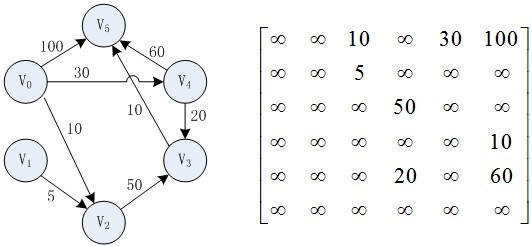
\includegraphics[width=240pt]{dijkstra.png}\\
\figcaption{有向图及其邻接矩阵}\label{fig:dijkstra}
\end{center}

运算过程中$v_0$到其余个顶点的最短路近,\fn{dist[]}向量的变化情况如表\ref{tab:dijkstra}所示(从一列到下一列只需要更新新加入点的邻接点)。

\begin{center}
\tabcaption{Dijkstra算法过程中dist[]向量的变化情况}
\label{tab:dijkstra}
\begin{tabular}{|c|ccccc|}
\hline
\textbf{\textbf{终点}} & \textbf{i=1} & \textbf{i=2} & \textbf{i=3} & \textbf{i=4} & \textbf{i=5}\\
\hline
$v_1$ & $\infty$ & $\infty$ & $\infty$ & $\infty$ & $\infty$\\
\hline
\multirow{2}{*}{$v_2$} & \textbf{10}          & & & & \\
                       & $\mathbf{(v_0,v_2)}$ & & & & \\
\hline
\multirow{2}{*}{$v_3$} & $\infty$ &          60     &     \textbf{50}          & & \\
                       &          & $(v_0,v_2,v_3)$ & $\mathbf{(v_0,v_4,v_5)}$ & & \\
\hline
\multirow{2}{*}{$v_4$} &     30      &      \textbf{30}     & & & \\
                       & $(v_0,v_4)$ & $\mathbf{(v_0,v_4)}$ & & & \\
\hline
\multirow{2}{*}{$v_5$} &     100     &     100     &       90        &         \textbf{60}          & \\
                       & $(v_0,v_5)$ & $(v_0,v_5)$ & $(v_0,v_4,v_5)$ & $\mathbf{(v_0,v_4,v_3,v_5)}$ & \\
\hline
$v_j$ & $v_2$ & $v_4$ & $v_3$ & $v_5$ & \\
\hline
$S$ & $(v_0,v_2)$ & $(v_0,v_2,v_4)$ & $(v_0,v_2,v_3,v_4)$ & $(v_0,v_2,v_3,v_4,v_5)$ & \\
\hline
\end{tabular}
\end{center}

Dijkstra算法的C语言实现如下。

\subsubsection{代码}

\begin{Codex}[label=mgraph_dijkstra.c]
#include <stdio.h>
#include <stdlib.h>  /* for malloc() */
#include <limits.h>  /* for INT_MAX */

/** 顶点数的最大值*/
#define MAX_VERTICES_NUM 100
/** 边的权值,对无权图,用0或1表示是否相邻;对有权图,则为权值. */
typedef int graph_weight_t;
#define GRAPH_INF INT_MAX

/**
 *@struct
 *@brief 邻接矩阵.
 */
typedef struct mgraph_t {
    int nv; /* 顶点数*/
    int ne; /* 边数*/
    /* 邻接矩阵,存放边的信息,如权重等*/
    graph_weight_t matrix[MAX_VERTICES_NUM][MAX_VERTICES_NUM];
} mgraph_t;

mgraph_t g;

/** path[i]存放的是最短路径上指向vi的弧尾顶点 */
int path[MAX_VERTICES_NUM];
/** dist[i]存放的是v到vi的最短路径长度 */
graph_weight_t dist[MAX_VERTICES_NUM];


/*
  * @brief Dijkstra算法求单源最短路径.
  * @param[in] g 图对象的指针
  * @param[in] v 起点
  * @param[out] dist dist[i]存放的是v到vi的最短路径长度
  * @param[out] path path[i]存放的是最短路径上指向vi的弧尾顶点
  * @return 无
  */
void mgraph_dijkstra(const mgraph_t *g, int v, graph_weight_t dist[], int path[]) {
    int i, j;
    const int n = g->nv;

    /* 初始化S集合 */
    int *S = (int*)calloc(n, sizeof(int));
    S[v] = 1; /* 初始化,顶点u加入S */

    /* 初始化dist和path */
    for(i = 0; i < n; i++) if (i !=v) {
        dist[i] = g->matrix[v][i];
        if(dist[i] < GRAPH_INF) {
            path[i] = v;
        }  else {
            path[i] = -1; /* 没有顶点指向i */
        }
    }
    dist[v] = 0;
    path[v] = -1;

    for(i = 0; i < n; i++) if (i !=v) {
        /* 选不在S中的最短路径顶点 u */
        int u = -1;
        graph_weight_t min = GRAPH_INF;
        for(j = 0; j < n; j++) {
            if(!S[j] && dist[j] < min) {
                u = j;
                min = dist[j];
            }
        }
        if (u < 0) break; /* 结束 */
        S[u] = 1;
        for(j = 0; j < n; j++) {
            const graph_weight_t w = g->matrix[u][j];
            /* 顶点j未就加入S,且经过u到j可缩短路径*/
            if(!S[j] && w < GRAPH_INF &&
                dist[u] + w < dist[j]) {
                dist[j] = dist[u] + w;
                path[j] = u; /* 修改到j的最短路径*/
            }
        }
    }
    free(S);
}

/*
 * @brief 打印从起点到v的最短路径
 * @param[in] v 终点
 * @param[in] path Dijkstra计算好的path
 * @return 无
 */
static void print_path_r(int v, const int path[]) {
    if (path[v] == -1) {
        printf("%c", 'A' + v);
    } else {
        print_path_r(path[v], path);
        printf("->%c", 'A' + v);
    }
}

/**
 * @brief 打印 u到其他所有点的最短路径
 * @param[in] path Dijkstra计算好的path
 * @param[in] n path的长度
 * @return 无
 */
void print_path(const int path[], int n) {
    int i;
    for (i = 0; i < n; i++) if (path[i] != -1) {
        print_path_r(i, path);
        printf("\n");
    }
}

/**
 * @brief 读取输入,构建图.
 */
void read_graph() {
    int i, j, k;

    /* 读取节点和边的数目 */
    scanf("%d%d", &g.nv, &g.ne);

    /* 初始化图,所有节点间距离为无穷大 */
    for (i = 0; i < g.nv; i++) {
        for (j = 0; j < g.nv; j++) {
            g.matrix[i][j] = GRAPH_INF;
        }
    }

    /* 读取边信息 */
    getchar(); // 消耗回车键
    for (k = 0; k < g.ne; k++) {
        char chx, chy;
        graph_weight_t w;
        scanf("%c %c %d", &chx, &chy, &w);
        getchar();
        i = chx - 'A';
        j = chy - 'A';
        g.matrix[i][j] = w;
    }
}

/* test

输入数据:

6 8
A C 10
A E 30
A F 100
B C 5
C D 50
D 5 10
E D 20
E F 60

输出:

A->C
A->E->D
A->E
A->E->F
*/
int main() {
    read_graph();

    /* 求 V0 到其他所有顶点的最短路径 */
    mgraph_dijkstra(&g, 0, dist, path);
    print_path(path, g.nv);
    return 0;
}
\end{Codex}

\subsubsection{算法分析}
该算法包含了两个并列的for循环,第一个for循环做辅助数组的初始化工作,计算时间为$O(n)$,第二个for循环是二重嵌套循环,进行最短路径的求解工作,由于对图中几乎每个顶点都要做计算,每个顶点的又要对集合S内的顶点进行检测,对集合$V-S$内中的顶点进行修改,所以运算时间复杂度为$O(n^2)$。算法总的时间复杂度为$O(n^2)$。


\subsection{每点最短路径——Floyd算法}
Floyd算法的基本思想是:假设求从定点$v_i$到$v_j$的最短路径。初始时,若$v_i$与$v_j$之间存在边,则最短路径长度为此边的权值;若不存在边,则最短路径长度为无穷大。以后逐步在路径中加入顶点$k(k=0,1,...,n-1)$作为中间顶点,如果加入中间顶点后,得到的路径比原来的路径长度减少了,则以新路径代替原路径。

首先比较$(v_i,v_j)$和$(v_i,v_0,v_j)$的路径长度,取较短者为从$v_i$到$v_j$的中间顶点的序号不大于0的最短路径。如果$(v_i,v_0,v_j)$较短,则取$(v_i,v_0,v_j)$作为最短路径。假如在路径上再增加一个顶点$v_1$,也就是说,如果$(v_i,...,v_1)$和$(v_1,...,v_j)$分别是当前找到的中间定点的序号不大于0的最短路径,那么$(vi,...,v1,...,vj)$就有可能是从$v_i$到$v_j$的中间顶点的序号不大于1的最短路径,将它和已经得到的从$v_i$到$v_j$的中间顶点的序号不大于0的最短路径相比较,选出较短者作为从$v_i$到$v_j$的中间顶点的序号不大于1的最短路径。再增加一个顶点$v_2$,继续进行试探,依此类推。一般的,若$(v_i,...,v_k)$和$(v_k,...,v_j)$分别是从$v_i$到$v_k$和从$v_k$到$v_j$的中间定点的序号不大于$k-1$的最短路径,则将$(v_i,...,v_k,...,v_j)$和已经得到的从$v_i$到$v_j$的中间顶点的序号不大于$k-1$的最短路径相比,较短者便是从$v_i$到$v_j$的中间顶点的序号不大于$k$的最短路径。这样,在经过$n$次比较后,最后求得的必是从$v_i$到$v_j$的最短路径。

现定义一个$n$阶方阵序列,
$$
D^{(-1)}, D^{(0)} , D^{(1)},..., , D^{(k)},..., , D^{(n-1)}
$$
其中,
\begin{eqnarray}
D^{(-1)}[i][j] &=& \text{g->matrix}[i][j],  \nonumber \\
D^{(k)}[i][j] &=& \min\left\{D^{(k-1)}[i][j], D^{(k-1)}[i][k] + D^{(k-1)}[k][j]\right\},0 \leq k \leq n-1 \nonumber
\end{eqnarray}

上述公式中,$D^{(k)}[i][j]$是从$v_i$到$v_j$的中间顶点的序号不大于$k$的最短路径的长度;$D^{(n-1)}[i][j]$是从$v_i$到$v_j$的最短路径的长度。

例如,对图\ref{fig:floyd}所示的有向图及其邻接矩阵运行Floyd算法,

\begin{center}
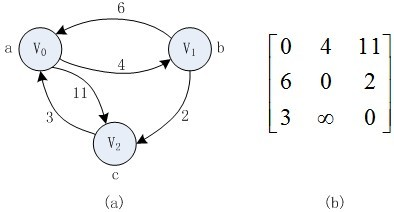
\includegraphics[width=180pt]{floyd.png}\\
\figcaption{有向图及其邻接矩阵}\label{fig:floyd}
\end{center}

运算过程中矩阵D的变化如表\ref{tab:floyd}所示。

\begin{center}
\tabcaption{Floyd算法过程中方阵和最短路径的变化}
\label{tab:floyd}
\begin{tabular}{|c|ccc|ccc|ccc|ccc|}
\hline
\multirow{2}{*}{$\mathbf{D}$} & \multicolumn{3}{|c|}{$\mathbf{D^{(0)}}$} & \multicolumn{3}{|c|}{$\mathbf{D^{(1)}}$} & \multicolumn{3}{|c|}{$\mathbf{D^{(2)}}$} & \multicolumn{3}{|c|}{$\mathbf{D^{(3)}}$} \\
 & 0 & 1 & 2 & 0 & 1 & 2 & 0 & 1 & 2 & 0 & 1 & 2 \\
\hline
0 & 0 & 4 & 11 & 0 & 4 & 11 & 0 & 4 & 6 & 0 & 4 & 6 \\
1 & 6 & 0 & 2 & 6 & 0 & 2 & 6 & 0 & 2 & 5 & 0 & 2 \\
2 & 3 & $\infty$ & 0 & 3 & 7 & 0 & 3 & 7 & 0 & 3 & 7 & 0 \\
\hline
\multirow{2}{*}{$\mathbf{P}$} & \multicolumn{3}{|c|}{$\mathbf{P^{(0)}}$} & \multicolumn{3}{|c|}{$\mathbf{P^{(1)}}$} & \multicolumn{3}{|c|}{$\mathbf{P^{(2)}}$} & \multicolumn{3}{|c|}{$\mathbf{P^{(3)}}$} \\
 & 0 & 1 & 2 & 0 & 1 & 2 & 0 & 1 & 2 & 0 & 1 & 2 \\
\hline
\multirow{2}{*}{0} & & A & A & & AB & A & & AB & AB & & AB & AB \\
                   & & B & C & & & C & & & C & & & C \\
\hline
\multirow{2}{*}{1} & B & & B & B & & B & B & & BC & BC & & BC \\
                   & A & & C & A & & C & A & & & A & & \\
\hline
\multirow{2}{*}{2} & C & & & C & CA & & C & CA & & CA & CA & \\
                   & A & & & A & B & & A & B & & & B & \\
\hline
\end{tabular}
\end{center}

Floyd算法的C语言实现如下。

\subsubsection{代码}

\begin{Codex}[label=mgraph_floyd.c]
#include <stdio.h>
#include <stdlib.h>  /* for malloc() */
#include <limits.h>  /* for INT_MAX */

/** 顶点数的最大值*/
#define MAX_VERTICES_NUM 100
/** 边的权值,对无权图,用0或1表示是否相邻;对有权图,则为权值. */
typedef int graph_weight_t;
#define GRAPH_INF (INT_MAX / 2)   /* 确保加法不溢出 */

/**
 *@struct
 *@brief 邻接矩阵.
 */
typedef struct mgraph_t {
    int nv; /* 顶点数*/
    int ne; /* 边数*/
    /* 邻接矩阵,存放边的信息,如权重等*/
    graph_weight_t matrix[MAX_VERTICES_NUM][MAX_VERTICES_NUM];
} mgraph_t;


mgraph_t g;
/** dist[i][j]是顶点i和j之间最短路径长度 */
graph_weight_t dist[MAX_VERTICES_NUM][MAX_VERTICES_NUM];
/** path[i][j]是最短路径上i和j之间的顶点 */
int path[MAX_VERTICES_NUM][MAX_VERTICES_NUM];


/*
  * @brief Floyd算法求每点之间最短路径.
  * @param[in] g 图对象的指针
  * @param[out] dist dist[i][j]是顶点i和j之间最短路径长度
  * @param[out] path path[i][j]是最短路径上i和j之间的顶点
  * @return 无
  */
void mgraph_floyd(const mgraph_t *g,
       graph_weight_t dist[][MAX_VERTICES_NUM],
       int path[][MAX_VERTICES_NUM]) {
    int i, j, k;
    const int n = g->nv;

    for(i = 0; i < n; i++) {
        for(j = 0; j < n; j++) {
            if(i != j) {
                dist[i][j] = g->matrix[i][j];
                path[i][j] = i;
            } else {
                dist[i][j] = 0;
                path[i][j] = -1;
            }
        }
    }
    for(k = 0; k < n; k++) {
        for(i = 0; i < n; i++) {
            for(j = 0; j < n; j++) {
                /* i到j的路径上加入顶点k可以缩短路径长度*/
                if(dist[i][k] + dist[k][j] < dist[i][j]) {
                    dist[i][j] = dist[i][k] + dist[k][j];
                    path[i][j] = k;
                }
            }
        }
    }
}

/*
 * @brief 打印从u到v的最短路径
 * @param[in] u 起点
 * @param[in] v 终点
 * @param[in] path Floyd 计算好的path
 * @return 无
 */
static void print_path_r(int u, int v, const int path[][MAX_VERTICES_NUM]) {
    if (path[u][v] == -1) {
        printf("%c", 'A' + u);
    } else {
        print_path_r(u, path[u][v], path);
        printf("->%c", 'A' + v);
    }
}

/**
 * @brief 打印 u到其他所有点的最短路径
 * @param[in] path Dijkstra计算好的path
 * @param[in] n path的长度
 * @return 无
 */
void print_path(const mgraph_t *g, const int path[][MAX_VERTICES_NUM]) {
    int i, j;
    for (i = 0; i < g->nv; i++) {
        for (j = 0; j < g->nv; j++) {
            if (i != j) {
                print_path_r(i, j, path);
                printf("\n");
            }
        }
        printf("\n");
    }
}

/**
 * @brief 读取输入,构建图.
 */
void read_graph() {
    int i, j, k;

    /* 读取节点和边的数目 */
    scanf("%d%d", &(g.nv), &(g.ne));

    /* 初始化图,所有节点间距离为无穷大 */
    for (i = 0; i < g.nv; i++) {
        for (j = 0; j < g.nv; j++) {
            g.matrix[i][j] = GRAPH_INF;
        }
    }

    /* 读取边信息 */
    getchar(); // 消耗回车键
    for (k = 0; k < g.ne; k++) {
        char chx, chy;
        graph_weight_t w;

        scanf("%c %c %d", &chx, &chy, &w);
        getchar();
        i = chx - 'A';
        j = chy - 'A';
        g.matrix[i][j] = w;
    }
}

/* test

输入数据:

3 5
A B 4
A C 11
B A 6
B C 2
C A 3

输出:

A->B
A->B->C

B->C->A
B->C

C->A
C->A->B
*/
int main() {
    read_graph();
    /* 求两两之间的最短路径 */
    mgraph_floyd(&g, dist, path);
    print_path(&g, path);
    return 0;
}
\end{Codex}

\subsubsection{算法分析}
该算法中有两个并列的for循环,第一个循环是个二重循环,用于初始化方阵$D$;第二个循环是个三重循环,逐步生成$D^{(0)}, D^{(1)} ,...,D^{(n-1)}$。所以算法总的时间复杂度为$O(n^3)$。

Dijkstra算法权值不能为负,Floyd权值可以为负,但环路之和不能为负。


\subsection{例题:HDU 2544 最短路}
\subsubsection{描述}
在每年的校赛里,所有进入决赛的同学都会获得一件很漂亮的t-shirt。但是每当我们的工作人员把上百件的衣服从商店运回到赛场的时候,却是非常累的!所以现在他们想要寻找最短的从商店到赛场的路线,你可以帮助他们吗?

\subsubsection{输入}
输入包括多组数据。每组数据第一行是两个整数$N,M(N \leq 100,M \leq 10000)$,$N$表示成都的大街上有几个路口,标号为1的路口是商店所在地,标号为$N$的路口是赛场所在地,$M$则表示在成都有几条路。$N=M=0$表示输入结束。接下来$M$行,每行包括3个整数$A,B,C(1 \leq A,B \leq N,1 \leq C \leq 1000)$,表示在路口$A$与路口$B$之间有一条路,我们的工作人员需要$C$分钟的时间走过这条路。
输入保证至少存在1条商店到赛场的路线。

\subsubsection{输出}
对于每组输入,输出一行,表示工作人员从商店走到赛场的最短时间

\subsubsection{样例输入}
\begin{Code}
2 1
1 2 3
3 3
1 2 5
2 3 5
3 1 2
0 0
\end{Code}

\subsubsection{样例输出}
\begin{Code}
3
2
\end{Code}

\subsubsection{分析}
单源最短路径,用Dijkstra算法,将第\S\ref{sec:dijkstra}节中的代码稍加修改即可。

注意,街道是双向的,所以给边赋值时要对称赋值。

\subsubsection{代码}
\begin{Codex}[label=hdu_2544.c]
/* HDU 2544 最短路, http://acm.hdu.edu.cn/showproblem.php?pid=2544 */

/* 等价于复制粘贴,这里为了节约篇幅,使用include,在OJ上提交时请用复制粘贴 */
#include "mgraph_dijkstra.c"  /* 见“图->最短路径”这节 */

// 1. 修改范围
#define MAX_VERTICES_NUM 100
// 2. 重写 read_graph()
// 3. 重写 main()

/** 读取输入,构建图. */
void read_graph() {
    int i, j, k;
    /* 读取节点和边的数目 */
    scanf("%d%d", &g.nv, &g.ne);

    /* 初始化图,所有节点间距离为无穷大 */
    for (i = 0; i < g.nv; i++) {
        for (j = 0; j < g.nv; j++) {
            g.matrix[i][j] = GRAPH_INF;
        }
    }

    /* 读取边信息 */
    for (k = 0; k < g.ne; k++) {
        int x, y;
        graph_weight_t w;
        scanf("%d %d %d", &x, &y, &w);
        i = x - 1;
        j = y - 1;
        g.matrix[i][j] = w;
        g.matrix[j][i] = w;  // 注意,街道是双向的
    }

}

int main() {
    while (1) {
        read_graph();
        if (g.nv <= 0 || g.ne <= 0) break;
        /* 求 商店(即路口1) 到其他所有顶点的最短路径 */
        mgraph_dijkstra(&g, 0, dist, path);
        /* 打印商店(即路口1)到赛场(即路口N)的最短路径长度 */
        printf("%d\n", dist[g.nv - 1]);
    }
    return 0;
}
\end{Codex}

\subsubsection{相关的题目}
与本题相同的题目:
\begindot
\item HDU 2544 最短路, \myurl{http://acm.hdu.edu.cn/showproblem.php?pid=2544}
\myenddot

与本题相似的题目:
\begindot
\item POJ 2253 Frogger, \myurl{http://poj.org/problem?id=2253}
\item POJ 3268 Silver Cow Party, \myurl{http://poj.org/problem?id=3268}
\item POJ 1797 Heavy Transportation, \myurl{http://poj.org/problem?id=1797}
\item POJ 1847 Tram, \myurl{http://poj.org/problem?id=1847}
\myenddot


\subsection{例题:POJ 1125 Stockbroker Grapevine}
\subsubsection{描述}
Stockbrokers are known to overreact to rumours. You have been contracted to develop a method of spreading disinformation amongst the stockbrokers to give your employer the tactical edge in the stock market. For maximum effect, you have to spread the rumours in the fastest possible way. 

Unfortunately for you, stockbrokers only trust information coming from their "Trusted sources" This means you have to take into account the structure of their contacts when starting a rumour. It takes a certain amount of time for a specific stockbroker to pass the rumour on to each of his colleagues. Your task will be to write a program that tells you which stockbroker to choose as your starting point for the rumour, as well as the time it will take for the rumour to spread throughout the stockbroker community. This duration is measured as the time needed for the last person to receive the information.

\subsubsection{输入}
Your program will input data for different sets of stockbrokers. Each set starts with a line with the number of stockbrokers. Following this is a line for each stockbroker which contains the number of people who they have contact with, who these people are, and the time taken for them to pass the message to each person. The format of each stockbroker line is as follows: The line starts with the number of contacts ($n$), followed by n pairs of integers, one pair for each contact. Each pair lists first a number referring to the contact (e.g. a '1' means person number one in the set), followed by the time in minutes taken to pass a message to that person. There are no special punctuation symbols or spacing rules. 

Each person is numbered 1 through to the number of stockbrokers. The time taken to pass the message on will be between 1 and 10 minutes (inclusive), and the number of contacts will range between 0 and one less than the number of stockbrokers. The number of stockbrokers will range from 1 to 100. The input is terminated by a set of stockbrokers containing 0 (zero) people. 

\subsubsection{输出}
For each set of data, your program must output a single line containing the person who results in the fastest message transmission, and how long before the last person will receive any given message after you give it to this person, measured in integer minutes. 

It is possible that your program will receive a network of connections that excludes some persons, i.e. some people may be unreachable. If your program detects such a broken network, simply output the message "disjoint". Note that the time taken to pass the message from person A to person B is not necessarily the same as the time taken to pass it from B to A, if such transmission is possible at all.

\subsubsection{样例输入}
\begin{Code}
3
2 2 4 3 5
2 1 2 3 6
2 1 2 2 2
5
3 4 4 2 8 5 3
1 5 8
4 1 6 4 10 2 7 5 2
0
2 2 5 1 5
7        
2 2 6 7 1
0  
3 1 5 2 8 4 7
0
2 2 9 4 10
2 3 8 4 7
2 5 8 6 3
7        
2 2 6 7 8
0  
3 1 5 2 8 4 7
0
2 2 9 4 10
2 3 8 4 7
2 5 8 6 3
0
\end{Code}

\subsubsection{样例输出}
\begin{Code}
3 2  
3 10
1 12
7 17
\end{Code}

\subsubsection{分析}
用Floyd算法求出每点之间的最短路径,输出距离最大的。

\subsubsection{代码}
\begin{Codex}[label=poj_1125.c]
/* poj 1125 Stockbroker Grapevine, http://poj.org/problem?id=1125 */

/* 等价于复制粘贴,这里为了节约篇幅,使用include,在OJ上提交时请用复制粘贴 */
#include "mgraph_floyd.c"  /* 见“图->最短路径”这节 */

// 1. 修改范围
#define MAX_VERTICES_NUM 100
// 2. 添加 max_len 数组
/** 存放每个点的最短路径的最长者 */
graph_weight_t max_len[MAX_VERTICES_NUM];
// 3. 添加 max_element()和min_element
// 4. 重写 read_graph()
// 5. 重写 main()

static int max_element(const graph_weight_t w[], int begin, int end) {
    int i;
    int max_value = -GRAPH_INF;
    int max_pos = -1;
    for (i = begin; i < end; i++) {
        if (max_value < w[i]) {
            max_value = w[i];
            max_pos = i;
        }
    }
    return max_pos;
}

static int min_element(const graph_weight_t w[], int begin, int end) {
    int i;
    int min_value = INT_MAX;
    int min_pos = -1;
    for (i = begin; i < end; i++) {
        if (min_value > w[i]) {
            min_value = w[i];
            min_pos = i;
        }
    }
    return min_pos;
}


/** 读取输入,构建图. */
void read_graph() {
    int i, j;
    scanf("%d", &(g.nv));
    g.ne = 0;

    /* 初始化图,所有节点间距离为无穷大 */
    for (i = 0; i < g.nv; i++) {
        for (j = 0; j < g.nv; j++) {
            g.matrix[i][j] = GRAPH_INF;
        }
    }

    /* 读取边信息 */
    for (i = 0; i < g.nv; i++) {
        int m;
        graph_weight_t w;
        scanf("%d", &m);
        g.ne += m;
        while (m--) {
            scanf("%d %d", &j, &w);
            --j;
            g.matrix[i][j] = w;
        }
    }
}

int main() {
    /* 读取顶点数 */
    while (1) {
        int i, min_pos;
        read_graph();
        if (g.nv == 0)
            break;

        /* 求两两之间的最短路径 */
        mgraph_floyd(&g, dist, path);

        /* 找最短路径的最长着 */
        for (i = 0; i < g.nv; i++) {
            max_len[i] = dist[i][max_element(dist[i], 0, g.nv)];
        }
        /* 找 max_len 的最小者 */
        min_pos = min_element(max_len, 0, g.nv);

        if (max_len[min_pos] == GRAPH_INF) {
            printf("disjoint\n");
        } else {
            printf("%d %d\n", min_pos + 1, max_len[min_pos]);
        }
    }
    return 0;
}
\end{Codex}

\subsubsection{相关的题目}
与本题相同的题目:
\begindot
\item POJ 1125 Stockbroker Grapevine, \myurl{http://poj.org/problem?id=1125}
\myenddot

与本题相似的题目:
\begindot
\item POJ 3615 Cow Hurdles, \myurl{http://poj.org/problem?id=3615}
\item POJ 3660 Cow Contest, \myurl{http://poj.org/problem?id=3660}
\item POJ 2502 Subway, \myurl{http://poj.org/problem?id=2502}
\item HDU 3631 Shortest Path, \myurl{http://acm.hdu.edu.cn/showproblem.php?pid=3631}
\myenddot


\section{拓扑排序} %%%%%%%%%%%%%%%%%%%%%%%%%%%%%%
由某个集合上的一个偏序得到该集合上的一个全序,这个操作称为\textbf{拓扑排序}。

拓扑序列的特点是:若有向边$<V_i, V_j>$是途中的弧,则在序列中顶点$V_i$必须排在顶点$V_j$之前。

如果用有向图表示一个工程,顶点表示活动,用有向边$<v_i,v_j>$表示活动必须先于活动进行。这种有向图叫做顶点表示活动的网络(Activity On Vertext Network),简称\textbf{AOV网络}。

检测AOV网络是否存在环的方法是对AOV网络构造其顶点的拓扑有序序列。拓扑排序的基本步骤是:
\begin{enumerate}
\item 在有向图中选一个没有前驱的顶点且输出之;
\item 从图中删除该顶点和所有以它为尾的弧线。
\end{enumerate}
重复以上两步,直至全部顶点输出,或当前图中不存在无前驱的顶点为止(这种情况说明图中存在环)。

拓扑排序的C语言实现如下。

\subsubsection{代码}

\begin{Codex}[label=mgraph_topo_sort.c]
#include <stdio.h>
#include <stdlib.h>  /* for malloc() */
#include <limits.h>  /* for INT_MAX */

/** 顶点数的最大值*/
#define MAX_VERTICES_NUM 100
/** 边的权值,对无权图,用0或1表示是否相邻;对有权图,则为权值. */
typedef int graph_weight_t;
#define GRAPH_INF INT_MAX

/**
 *@struct
 *@brief 邻接矩阵.
 */
typedef struct mgraph_t {
    int nv; /* 顶点数*/
    int ne; /* 边数*/
    /* 邻接矩阵,存放边的信息,如权重等*/
    graph_weight_t matrix[MAX_VERTICES_NUM][MAX_VERTICES_NUM];
} mgraph_t;

mgraph_t g;
/** 拓扑排序的结果. */
int topological[MAX_VERTICES_NUM];

/* 等价于复制粘贴,这里为了节约篇幅,使用include,在OJ上提交时请用复制粘贴 */
#include "stack.c"  /* 见“栈和队列->栈”这节 */

/*
  * @brief 拓扑排序.
  * @param[in] g 图对象的指针
  * @param[out] topological 保存拓扑排序的结果
  * @return 无环返回 1,有环返回 0
  */
int mgraph_topo_sort(const mgraph_t *g, int topological[]) {
    int i, j, u;
    int count = 0; /* 拓扑序列的元素个数*/
    const int n = g->nv;
    /* in_degree[i]是顶点i的入度 */
    int *in_degree = (int*)malloc(n * sizeof(int));
    stack_t *s = stack_create(n * sizeof(int));

    memset(in_degree, 0, n * sizeof(int));
    for (i = 0; i < n; i++) {
        for (j = 0; j < n; j++) {
            if (g->matrix[i][j] < GRAPH_INF)
                in_degree[j]++;
        }
    }

    for(i = 0; i < n; i ++) {
        if(in_degree[i] == 0)
            stack_push(s, i);
    }

    while(!stack_empty(s)) {
        u = stack_top(s); stack_pop(s);
        topological[count++] = u;
        for (i = 0; i < n; i++) if (g->matrix[u][i] < GRAPH_INF) {
            if(--in_degree[i] == 0) stack_push(s, i);
        }
    }

    free(in_degree);
    stack_destroy(s);
    if(count != n) { /* 有环*/
        return 0;
    } else { /* 无环*/
        return 1;
    }
}

/** 读取输入,构建图. */
void read_graph() {
    int i, j, k;
    char buf[10]; /* 和 gets()配合消除回车键 */
    /* 读取节点和边的数目 */
    scanf("%d %d", &g.nv, &g.ne);
    gets(buf); // 消耗回车键

    /* 初始化图,所有节点间距离为无穷大 */
    for (i = 0; i < g.nv; i++) {
        for (j = 0; j < g.nv; j++) {
            g.matrix[i][j] = GRAPH_INF;
        }
    }

    /* 读取边信息 */
    for (k = 0; k < g.ne; k++) {
        char chx, chy;
        graph_weight_t w;
        scanf("%c %c %d", &chx, &chy, &w);
        gets(buf); // 消耗回车键
        i = chx - 'A';
        j = chy - 'A';
        g.matrix[i][j] = w;
    }
}

/* test

输入数据:

6 8
A C 10
A E 30
A F 100
B C 5
C D 50
D 5 10
E D 20
E F 60

输出:

B A E F C D
*/
int main() {
    int i;
    read_graph();
    /* 拓扑排序 */
    mgraph_topo_sort(&g, topological);
    for (i = 0; i < g.nv; i++) {
        printf("%c ", 'A'+topological[i]);
    }
    return 0;
}
\end{Codex}

\subsubsection{算法分析}
对有$n$个顶点和$e$条边的AOV网络而言,求各顶点的入度所需时间为$O(e)$,建立零入度顶点栈所需时间为$O(n)$;在拓扑排序过程中,若有向图无环,每个顶进一次栈出一次栈,顶点入度减1的操作共执行了$e$次。所以总的时间复杂度为$O(n+e)$。

当有向图中无环时,也可以利用深度优先搜索进行拓扑排序。因为图中无环,深度优先遍历不会死循环。进行深度优先遍历时,最先退出DFS函数的顶点即为出度为零的顶点,是拓扑有序序列的最后一个顶点。由此,按退出DFS函数的先后次序记录下来的顶点序列即为逆向的拓扑有序序列。


\subsection{例题:POJ 1094 Sorting It All Out}
\subsubsection{描述}
An ascending sorted sequence of distinct values is one in which some form of a less-than operator is used to order the elements from smallest to largest. For example, the sorted sequence $A, B, C, D$ implies that $A < B, B < C$ and $C < D$. in this problem, we will give you a set of relations of the form $A < B$ and ask you to determine whether a sorted order has been specified or not.

\subsubsection{输入}
Input consists of multiple problem instances. Each instance starts with a line containing two positive integers $n$ and $m$. the first value indicated the number of objects to sort, where $2 \leq n \leq 26$. The objects to be sorted will be the first $n$ characters of the uppercase alphabet. The second value $m$ indicates the number of relations of the form $A < B$ which will be given in this problem instance. Next will be $m$ lines, each containing one such relation consisting of three characters: an uppercase letter, the character "<" and a second uppercase letter. No letter will be outside the range of the first $n$ letters of the alphabet. Values of $n = m = 0$ indicate end of input.

\subsubsection{输出}
For each problem instance, output consists of one line. This line should be one of the following three: 

Sorted sequence determined after $xxx$ relations: $yyy...y$.

Sorted sequence cannot be determined. 

Inconsistency found after $xxx$ relations.

where $xxx$ is the number of relations processed at the time either a sorted sequence is determined or an inconsistency is found, whichever comes first, and $yyy...y$ is the sorted, ascending sequence.

\subsubsection{样例输入}
\begin{Code}
4 6
A<B
A<C
B<C
C<D
B<D
A<B
3 2
A<B
B<A
26 1
A<Z
6 6
A<F
B<D
C<E
F<D
D<E
E<F
0 0
\end{Code}

\subsubsection{样例输出}
\begin{Code}
Sorted sequence determined after 4 relations: ABCD.
Inconsistency found after 2 relations.
Sorted sequence cannot be determined.
Inconsistency found after 6 relations.
\end{Code}

\subsubsection{分析}
根据题目的要求,我们要每输入一次就要进行一次拓扑排序\fn{topological_sort()},这样才能做到不成功(即发现有环)时,能知道是哪步不成功,并且给出输出。

还有要注意的就是如果我们可以提前判断结果了,但后面还有输入没完成,那么我们必须继续完成输入,不然剩下的输入会影响下一次case的输入。

\subsubsection{代码}
\begin{Codex}[label=poj_1094.c]
#include <stdio.h>
#include <stdlib.h>  /* for malloc() */
#include <limits.h>  /* for INT_MAX */

/** 顶点数的最大值*/
#define MAX_VERTICES_NUM 26
/** 边的权值,对无权图,用0或1表示是否相邻;对有权图,则为权值. */
typedef int graph_weight_t;
#define GRAPH_INF INT_MAX

/**
 *@struct
 *@brief 邻接矩阵.
 */
typedef struct mgraph_t {
    int nv; /* 顶点数*/
    int ne; /* 边数*/
    /* 邻接矩阵,存放边的信息,如权重等*/
    graph_weight_t matrix[MAX_VERTICES_NUM][MAX_VERTICES_NUM];
} mgraph_t;

mgraph_t g;
/** 拓扑排序的结果. */
int topological[MAX_VERTICES_NUM];

/* 等价于复制粘贴,这里为了节约篇幅,使用include,在OJ上提交时请用复制粘贴 */
#include "stack.c"  /* 见“栈和队列->栈”这节 */

/**
  * @brief 拓扑排序.
  * @param[in] g 图对象的指针
  * @param[out] topological 保存拓扑排序的结果
  * @return 无环返回 1,有环返回 0
  */
int mgraph_topological_sort(const mgraph_t *g, int topological[]) {
    int i, j, u;
    int count = 0; /* 拓扑序列的元素个数*/
    int insufficient = 0;  /* 条件不足 */
    const int n = g->nv;
    /* in_degree[i]是顶点i的入度 */
    int *in_degree = (int*)malloc(n * sizeof(int));
    stack_t *s = stack_create(n * sizeof(int));

    memset(in_degree, 0, n * sizeof(int));
    for (i = 0; i < n; i++) {
        for (j = 0; j < n; j++) {
            if (g->matrix[i][j] < GRAPH_INF)
                in_degree[j]++;
        }
    }

    for(i = 0; i < n; i ++) {
        if(in_degree[i] == 0) {
            stack_push(s, i);
        }
    }

    while(!stack_empty(s)) {
        // 栈内应该始终只有一个元素
        if (stack_size(s) > 1) insufficient = 1;
        // 删除顶点u
        u = stack_top(s); stack_pop(s);
        topological[count++] = u;
        --in_degree[u];  // 变成 -1,表示已经输出
        // 更新入度
        for (i = 0; i < n; i++) if (g->matrix[u][i] < GRAPH_INF) {
            --in_degree[i];
        }
        // 选择入度为0的顶点
        for (i = 0; i < n; i++) if (g->matrix[u][i] < GRAPH_INF) {
            if (in_degree[i] == 0) stack_push(s, i);
        }
    }

    free(in_degree);
    stack_destroy(s);
    if(count < n) { /* 有环*/
        return 0;
    } else { /* 无环*/
        if (insufficient) {  /* 有孤立点,说明条件不足 */
            return -1;
        } else {
            return 1;
        }
    }
}

int main() {
    int i, j, k, m;  // m不一定是边的数目,因为输入边可能有重复

    /* 读取节点和边的数目 */
    while (scanf("%d %d", &(g.nv), &m)
            && g.nv > 0 && m > 0) {
        char s[4];
        int ok;  // 是否有环,0 表示有环
        int finished = 0;  // 排序完成,结束,发现有环,可以提前结束

        /* 初始化图,所有节点间距离为无穷大 */
        for (i = 0; i < g.nv; i++) {
            for (j = 0; j < g.nv; j++) {
                g.matrix[i][j] = GRAPH_INF;
            }
        }

        /* 读取边信息 */
        for (k = 0; k < m; k++) {
            scanf("%s", s);
            i = s[0] - 'A';
            j = s[2] - 'A';
            g.matrix[i][j] = 1;

            if (finished) continue;    // 完成,则 continue,消耗输入

            /* 拓扑排序 */
            ok = mgraph_topological_sort(&g, topological);

            if (ok == 0) {  // 有环存在
                printf("Inconsistency found after %d relations.\n", k + 1);
                finished = 1;  // 提前结束,记住要继续消耗输入
            }
            if (ok == 1 && k) {
                printf("Sorted sequence determined after %d relations: ", k+1);
                for (i = 0; i < g.nv; i++) {
                    printf("%c", 'A' + topological[i]);
                }
                printf(".\n");
                finished = 1;
            }
            // ok==-1, continue
        }
        if (finished == 0) {
            printf("Sorted sequence cannot be determined.\n");
        }
    }
    return 0;
}
\end{Codex}

\subsubsection{相关的题目}
与本题相同的题目:
\begindot
\item POJ 1094 Sorting It All Out, \myurl{http://poj.org/problem?id=1094}
\myenddot

与本题相似的题目:
\begindot
\item POJ 3267 The Cow Lexicon, \myurl{http://poj.org/problem?id=3267}
\item POJ 3687 Labeling Balls, \myurl{http://poj.org/problem?id=3687}
\myenddot


\section{关键路径} %%%%%%%%%%%%%%%%%%%%%%%%%%%%%%
用有向边上的权值表示活动的持续时间,用顶点表示时间,这样的有向图叫做边表示的活动网络(Activity On Edge Network),简称\textbf{AOE网络}。

路径最长的路径叫做\textbf{关键路径}(Critical Path)。假设开始点为$v_1$,从$v_1$到$v_i$的最长路径长度叫做事件$v_i$的最早发生时间。这个事件决定了所有以$v_i$为尾的弧所表示的活动的最早开始时间。我们用$e(i)$表示活动$a_i$的最早开始时间。还可以定义一个活动的最迟开始时间$l(i)$,这是在不推迟整个工程完成的前提下,活动$a_i$最迟必须开始进行的时间。两者之差$l(i)-e(i)$意味着完成活动$a_i$的时间余量。我们把$l(i)=e(i)$的活动叫做关键活动。

设活动$a_i$由弧$<j, k>$表示,为了求得活动的$e(i)$和$l(i)$,首先应求得事件的最早发生时间$ve(j)$和最迟发生时间$vl(j)$,其持续时间记为$dut(<j, k>)$,则有如下关系
\begin{eqnarray}
e(i) &=& ve(j) \nonumber \\
l(i) &=& vl(k)-dut(<j, k>) \nonumber
\end{eqnarray}

求$ve(j)$和$vl(k)$需分两步进行:
\begin{enumerate}
\item 从$ve(0)=0$开始向前递推
$$
ve(j)=\max\left\{ve(i)+dut(<i, j>)\right\}, <i, j> \in T
$$
其中$T$是所有以顶点$j$为弧头的边的集合。
\item 从$vl(n-1)=ve(n-1)$起向后递推
$$
vl(j)=\min\left\{vl(k)-dut(<j, k>)\right\}, <j, k> \in S
$$
其中$S$是所有以顶点$j$为弧尾的边的集合。
\end{enumerate}

例如,对图\ref{fig:criticalpath}(a)所示AOE网络的计算过程如表\ref{tab:criticalpath}所示,可见$a_2$、$a_5$和$a_7$为关键活动,组成一条从起点到终点的关键路径,如图\ref{fig:criticalpath}(b)所示。

\begin{center}
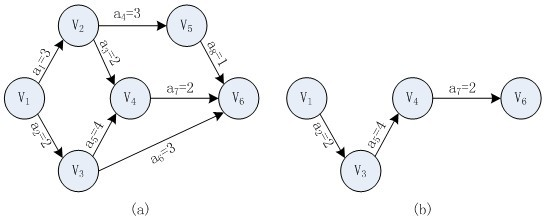
\includegraphics[width=240pt]{criticalpath.png}\\
\figcaption{有向图及其邻接矩阵}\label{fig:criticalpath}
\end{center}

\begin{center}
\tabcaption{图\ref{fig:criticalpath}(a)所示AOE网络的关键路径的计算过程}
\label{tab:criticalpath}
\begin{tabular}{|ccccc|cccc|}
\hline
\textbf{顶点} & \textbf{ve} & & \textbf{vl} & & \textbf{活动} & \textbf{e} & \textbf{l} & \textbf{l-e} \\
\hline
$v_1$ & 0 & \multirow{8}{*}{$\downarrow$} & 0 & \multirow{8}{*}{$\uparrow$} & $a_1$ & 0 & 1 & 1 \\
$v_2$ & 3 &                               & 4 &                             & $a_2$ & 0 & 0 & 0 \\
$v_3$ & 2 &                               & 2 &                             & $a_3$ & 3 & 4 & 1 \\
$v_4$ & 6 &                               & 6 &                             & $a_4$ & 3 & 4 & 1 \\
$v_5$ & 6 &                               & 7 &                             & $a_5$ & 2 & 2 & 0 \\
$v_6$ & 8 &                               & 8 &                             & $a_6$ & 2 & 5 & 3 \\
      &   &                               &   &                             & $a_7$ & 6 & 6 & 0 \\
      &   &                               &   &                             & $a_8$ & 6 & 7 & 1 \\
\hline
\end{tabular}
\end{center}


邻接矩阵上的关键路径的C语言实现如下。

\subsubsection{代码}

\begin{Codex}[label=mgraph_critical_path.c]
#include <stdio.h>
#include <stdlib.h>  /* for malloc() */
#include <limits.h>  /* for INT_MAX */

/** 顶点数的最大值*/
#define MAX_VERTICES_NUM 100
/** 边的权值,对无权图,用0或1表示是否相邻;对有权图,则为权值. */
typedef int graph_weight_t;
#define GRAPH_INF INT_MAX

/**
 *@struct
 *@brief 邻接矩阵.
 */
typedef struct mgraph_t {
    int nv; /* 顶点数*/
    int ne; /* 边数*/
    /* 邻接矩阵,存放边的信息,如权重等*/
    graph_weight_t matrix[MAX_VERTICES_NUM][MAX_VERTICES_NUM];
} mgraph_t;

mgraph_t g;
/** 拓扑排序的结果. */
int topological[MAX_VERTICES_NUM];
/** 关键路径,其余顶点为-1. */
int path[MAX_VERTICES_NUM];

/* 等价于复制粘贴,这里为了节约篇幅,使用include,在OJ上提交时请用复制粘贴 */
#include "stack.c"  /* 见“栈和队列->栈”这节 */

/*
  * @brief 按照拓扑排序的顺序,计算所有顶点的最早发生时间 ve.
  * @param[in] g 图对象的指针
  * @param[out] topological 保存拓扑排序的结果
  * @param[out] ve 所有事件的最早发生时间
  * @return 无环返回 1,有环返回 0
  */
static int mgraph_toposort_ve(const mgraph_t *g, int topological[],
        graph_weight_t ve[]) {
    int i, j, u;
    int count = 0; /* 拓扑序列的元素个数*/
    const int n = g->nv;
    /* in_degree[i]是顶点i的入度 */
    int *in_degree = (int*)malloc(n * sizeof(int));
    stack_t *s = stack_create(n * sizeof(int));

    memset(in_degree, 0, n * sizeof(int));
    for (i = 0; i < n; i++) {
        for (j = 0; j < n; j++) {
            if (g->matrix[i][j] < GRAPH_INF)
                in_degree[j]++;
        }
    }

    for(i = 0; i < n; i ++) {
        if(in_degree[i] == 0) {
            stack_push(s, i);
        }
    }

    memset(ve, 0, n * sizeof(graph_weight_t));

    while(!stack_empty(s)) {
        // 删除顶点u
        u = stack_top(s); stack_pop(s);
        topological[count++] = u;
        --in_degree[u];  // 变成 -1,表示已经输出
        // 更新入度
        for (i = 0; i < n; i++) if (g->matrix[u][i] < GRAPH_INF) {
            --in_degree[i];
        }
        // 更新邻接点的 ve
        for (i = 0; i < n; i++) if (g->matrix[u][i] < GRAPH_INF) {
            if (ve[i] < ve[u] + g->matrix[u][i])
                ve[i] = ve[u] + g->matrix[u][i];
        }
        // 选择入度为0的顶点
        for (i = 0; i < n; i++) if (g->matrix[u][i] < GRAPH_INF) {
            if (in_degree[i] == 0) stack_push(s, i);
        }
    }

    free(in_degree);
    stack_destroy(s);
    if(count < n) { /* 有环*/
        return 0;
    } else { /* 无环*/
        return 1;
    }
}

/**
  * @brief 求关键路径,第一个顶点为起点,最后一个顶点为终点.
  * @param[in] g 图对象的指针
  * @param[out] ve 所有事件的最早发生时间
  * @param[inout] path 关键路径
  * @return 无环返回关键路径的顶点个数,有环返回 0
  */
int mgraph_critical_path(const mgraph_t *g, int path[MAX_VERTICES_NUM]) {
    int i, j;
    int count = 0;    // 关键路径的顶点个数
    graph_weight_t *ve = (graph_weight_t*) malloc(
            g->nv * sizeof(graph_weight_t));
    graph_weight_t *vl = (graph_weight_t*) malloc(
            g->nv * sizeof(graph_weight_t));

    if (!mgraph_toposort_ve(g, topological, ve)) return 0;  // 有环

    for (i = 0; i < MAX_VERTICES_NUM; i++) path[i] = -1;
    // 初始化 vl 为最大
    for (i = 0; i < g->nv; i++) vl[i] = ve[g->nv-1];

    // 逆序计算vl
    for (i = g->nv-1; i >=0; i--) {
        int k = topological[i];
        for (j = 0; j < g->nv; j++) {
            if (g->matrix[j][k] < GRAPH_INF) {
                if (vl[j] > vl[k] - g->matrix[j][k])
                    vl[j] = vl[k] - g->matrix[j][k];
            }
        }
    }
    for (i = 0; i < g->nv; i++) {
        for (j = 0; j < g->nv; j++) {
            int e = ve[i];
            int l = vl[j] - g->matrix[i][j];
            if (e == l) {
                if (i == 0) {
                    path[count++] = i;
                    path[count++] = j;
                } else {
                    path[count++] = j;
                }
            }
        }
    }

    free(ve);
    free(vl);
    return count;
}

/** 读取输入,构建图. */
void read_graph() {
    int i, j, k;

    /* 读取节点和边的数目 */
    scanf("%d%d", &g.nv, &g.ne);

    /* 初始化图,所有节点间距离为无穷大 */
    for (i = 0; i < g.nv; i++) {
        for (j = 0; j < g.nv; j++) {
            g.matrix[i][j] = GRAPH_INF;
        }
    }

    /* 读取边信息 */
    getchar(); // 消耗回车键
    for (k = 0; k < g.ne; k++) {
        char chx, chy;
        graph_weight_t w;
        scanf("%c %c %d", &chx, &chy, &w);
        getchar();
        i = chx - 'A';
        j = chy - 'A';
        g.matrix[i][j] = w;
    }
}

/* test

输入数据:
6 8
A B 3
A C 2
C D 4
B D 2
C F 3
B E 3
E F 1
D F 2

输出: A C D F

*/
int main() {
    int i, count;
    read_graph();
    /* 拓扑排序 */
    count = mgraph_critical_path(&g, path);
    for (i = 0; i < count; i++) {
        printf("%c ", 'A' + path[i]);
    }
    return 0;
}
\end{Codex}

\subsubsection{算法分析}
一次正向,复杂度为$O(n^2)$,一次逆向,复杂度为$O(n^2)$,因此,该算法的复杂度为$O(n^2)$。

\chapter{数学方法与常见模型}
数学对于算法很重要。没有好的数学基础,很难在算法上达到一定高度。本章介绍算法竞赛中常用的数学方法和模型。

\section{数论} %%%%%%%%%%%%%%%%%%%%%%%%%%%%%%

\subsection{欧几里德算法}

求最大公约数(greates common divisor)有很多方法,最经典的方法是欧几里德算法(Euclidean algorithm\footnote{\myurl{http://en.wikipedia.org/wiki/Euclid_algorithm}}),又称辗转相除法。

\begin{Codex}[label=gcd.c]
/**
 * @brief 求最大公约数,欧几里德算法,也即辗转相除法
 *
 * @param[in] a a
 * @param[in] b b
 * @return a和b的最大公约数
 */
unsigned int gcd(unsigned int a, unsigned int b) {
    if (b == 0) return a;
    return gcd(b, a % b);
}

/**
 * @brief 求最大公约数,欧几里德算法,迭代版本
 *
 * @param[in] a a
 * @param[in] b b
 * @return a和b的最大公约数
 */
unsigned int gcd1(unsigned int a, unsigned int b) {
    while (b != 0) {
        unsigned int tmp = b;
        b = a % b;
        a = tmp;
    }
    return a;
}

/**
 * @brief 求最大公约数,欧几里德算法,迭代版本,基于减法
 *
 * @param[in] a a
 * @param[in] b b
 * @return a和b的最大公约数
 */
unsigned int gcd2(unsigned int a, unsigned int b) {
    while (a != b) {
        if (a > b) {
            a -= b;
        } else {
            b -= a;
        }
    }
    return a;
}
\end{Codex}

求出了最大公约数,可以利用它来求最小公倍数(least common multiple), $\mathrm{lcm}(a,b)=a \times b / \gcd(a,b)$。

\subsubsection{例题}
\begindot
\item wikioi 1212 最大公约数 ,\myurl{http://www.wikioi.com/problem/1212/}
\myenddot


\subsection{扩展欧几里德算法}
定理:对于不完全为$0$的非负整数$a,b$,必然存在整数对 $x,y$ ,使得 $\gcd(a,b)=ax+by$。

这里$x$和$y$不一定是正数。扩展欧几里德算法(Extended Euclidean algorithm\footnote{\myurl{http://en.wikipedia.org/wiki/Extended_Euclidean_algorithm}})就是用来求$x$和$y$的。

\begin{Codex}[label=ex_gcd.c]
/**
 * @brief 扩展欧几里德算法
 * @param[in] a a
 * @param[in] b b
 * @param[out] x
 * @param[out] y
 * @return gcd(a,b)
 */
unsigned int ex_gcd(unsigned int a, unsigned int b, int *x, int *y) {
    if(b == 0) {
        *x = 1; *y = 0; return a;
    } else {
        const unsigned int tmp = ex_gcd(b, a % b, y, x);
        *y -= (*x)*(a/b);
        return tmp;
    }
}
\end{Codex}

扩展欧几里德算法的应用主要有以下三个:
\begindot
\item 求解不定方程;
\item 求解模线性方程(线性同余方程);
\item 求解模的逆元;
\myenddot


\subsubsection{求解不定方程}
求不定方程$ax+by=c$的整数解$x,y$,其中$a > b \geq c \geq 0$。

设$g=\gcd(a,b)$,方程$ax+by=g$的一组解是$(x_0,y_0)$,则当$c$是$g$的倍数时$ax+by=c$的一组解是$(x_0,y_0)$。证明略。

\begin{Code}
/**
 * @brief 求解不定方程ax+by=c
 * @param[in] a a
 * @param[in] b b
 * @param[in] c c
 * @param[out] x x
 * @param[out] y y
 * @return 是否有解,1表示有解,0表示无解
 */
int linear_equation(unsigned int a, unsigned int b, unsigned int c,
        int *x, int *y) {
    unsigned int k;
    const unsigned int g = ex_gcd(a, b, x, y);
    if (c % g) return 0;

    k = c / g;
    (*x) *= k; (*y) *= k;
    return 1;
}
\end{Code}


\subsubsection{求解模线性方程}
解方程$ax \equiv b\bmod n$,其中$a,b,n$是正整数。

$ax \equiv b\bmod n$的含义是“$ax$和$b$除以$n$的余数相同”,设这个倍数为$y$,则$ax-b=ny$,这恰好就是前面介绍过的不定方程。接下来的步骤就不用说了吧。

\begin{Code}
/**
 * @brief 求解模线性方程 ax = b mod n
 * @param[in] a
 * @param[in] b
 * @param[in] n n>0
 */
int modular_linear_equation(unsigned int a, unsigned int b, unsigned int n) {
    int x, y, x0, i;
    unsigned int k;
    unsigned int g = ex_gcd(a, n, &x, &y);
    if(b % g) return 0;

    k = b / g;
    x0 = (k * x) % n;   //特解
    for (i = 0; i < g; i++)
        printf("%d\n", (x0 + i * (n/g)) % n);
    return 1;
}
\end{Code}


\subsubsection{求解模的逆元}
有一个特殊情况要引起读者重视,当$b=1$时,$ax \equiv 1\bmod n$的解称为$a$关于模$n$的逆(inverse),它类似于“倒数”的概念。什么时候$a$的逆存在呢?根据上面的讨论,方程$ax-ny=1$要有解,这样,1必须是$\gcd(a,n)$的倍数,因此$a$和$n$必须互素。

\subsection{素数判定}
素数判定,又称素数测试(Primality test\footnote{\myurl{http://en.wikipedia.org/wiki/Primality_test}}),即给定一个正整数$n$,判断它是否是素数。

\subsubsection{暴力枚举法}
从2到$n$,依次作为除数,让$n$除以它们,只要有一个能整除$n$,则$n$不是素数。

\begin{Code}
/**
 * @brief 判断正整数n是否是素数
 * @param[in] n 正整数
 * @return 是,返回1,否,返回0
 */
int is_prime(unsigned int n) {
    int i;
    if (n < 2) return 0;
    for (i = 2; i < n; i++) {
        if (n % i == 0) return 0;
    }
    return 1;
}
\end{Code}

可以稍微做一点改进,从1到$\sqrt n$,依次作为除数。

\begin{Code}
/**
 * @brief 判断正整数n是否是素数,上界改为sqrt(n)
 * @param[in] n 正整数
 * @return 是,返回1,否,返回0
 */
int is_prime(unsigned int n) {
    int i;
    if (n < 2) return 0;
    const int upper = sqrt(n);

    for (i = 2; i <= upper; i++) {
        if (n % i == 0) return 0;
    }
    return 1;
}

/**
 * @brief 判断正整数n是否是素数,上界改为sqrt(n),但不使用sqrt()函数
 * @param[in] n 正整数
 * @return 是,返回1,否,返回0
 */
int is_prime1(unsigned int n) {
    int i;
    if (n < 2) return 0;
    for (i = 2; i*i <= n; i++) {
        if (n % i == 0) return 0;
    }
    return 1;
}
\end{Code}

\subsubsection{Eratosthenes筛法}
更高效的素数判定方法应该是预先计算出一张素数表,当判断一个数是否是素数时,直接查表即可。

怎样计算?用Eratosthenes筛法(Sieve of Eratosthenes\footnote{\myurl{http://en.wikipedia.org/wiki/Sieve_of_Eratosthenes}})

给出要筛数值的范围$n$,找出$\sqrt{n}$以内的素数$p_{1},p_{2},\dots,p_{k}$。先用2去筛,即把2留下,把2的倍数剔除掉;再用下一个质数,也就是3筛,把3留下,把3的倍数剔除掉;接下去用下一个质数5筛,把5留下,把5的倍数剔除掉;不断重复下去......。

\begin{Code}
#define MAXN 30000
/** prime_table[i]==1表示i是素数,等于0则不是素数 */
int prime_table[MAXN+1];

void compute_prime_table() {
    int i, j;
    const int upper = sqrt(MAXN);

    for (i = 2; i <= MAXN; i++) prime_table[i] = 1;
    prime_table[0] = 0;
    prime_table[1] = 0;

    for (i = 2; i < upper; i++) if(prime_table[i]) {
        for (j = 2; j * i <= MAXN; j++) prime_table[j*i] = 0;
    }
}

int is_prime(unsigned int n) {
    return prime_table[n];
}
\end{Code}

\subsubsection{暴力枚举法优化版}
下面这段代码是从 GNU GMP(\myurl{http://gmplib.org/})的源代码中抠出来的。

\begin{Code}
int is_prime(unsigned int n) {
    unsigned int q, r, d;    /* 商,余数,除数 */

    /* 把这个常数展开成二进制就容易理解了 */
    if (n < 32) return (0xa08a28acUL >> n) & 1;
    if ((n & 1) == 0) return 0;
    if (n % 3 == 0) return 0;
    if (n % 5 == 0) return 0;
    if (n % 7 == 0) return 0;

    for (d = 11;;) {
        q = n / d;
        r = n - q * d;
        if (q < d) return 1;    /* 保证 d 不超过 sqrt(n) */
        if (r == 0) break;

        d += 2;
        q = n / d;
        r = n - q * d;
        if (q < d) return 1;
        if (r == 0) break;

        d += 4;
    }
    return 0;
}
\end{Code}


\subsubsection{例题}
\begindot
\item wikioi 1430 素数判定,\myurl{http://www.wikioi.com/problem/1430/}
\myenddot


\subsection{大整数取模} %%%%%%%%%%%%%%%%%%%%%%%%%%%%%%
\subsubsection{描述}
求$a \bmod b, 1 \leq a \leq 10^{1000},1 \leq b \leq 100000$。

\subsubsection{输入}
每行2个整数$a$和$b$

\subsubsection{输出}
对每一行输出结果 $a \bmod b$

\subsubsection{样例输入}
\begin{Code}
2 3
12 7
152455856554521 3250
\end{Code}

\subsubsection{样例输出}
\begin{Code}
2
5
1521
\end{Code}

\subsubsection{代码}
\begin{Codex}[label=bigint_mod.c]
#include<stdio.h>
#include<string.h>

/* 一个数组元素表示4个十进制位,即数组是万进制的 */
#define BIGINT_MOD 10000
#define MOD_LEN 4
#define MAX_LEN (1000/MOD_LEN+1)  /* 整数的最大位数 */

char    a[MAX_LEN * MOD_LEN];
int     x[MAX_LEN], y;

/**
 * @brief 将输入的字符串转化为大整数,用数组表示,低位在低地址.
 * @param[in] s 输入的字符串
 * @param[out] x 大整数
 * @return 无
 */
void bigint_input(const char s[], int x[]) {
    int i, j = 0;
    const int len = strlen(s);
    for (i = 0; i < MAX_LEN; i++) x[i] = 0;

    /* for (i = len - 1; i >= 0; i--) a[j++] = s[i] - '0'; */
    for (i = len; i > 0; i -= MOD_LEN) {  /* [i-MOD_LEN, i) */
        int temp = 0;
        int k;
        const int low = i-MOD_LEN > 0 ? i-MOD_LEN : 0;
        for (k = low; k < i; k++) {
            temp = temp * 10 + s[k] - '0';
        }

        x[j++] = temp;
    }
}

/**
 * @brief 计算 x mod y
 * @param[in] x 大整数
 * @param[in] y 模
 * @return x mod y
 */
int bigint_mod(const int x[MAX_LEN], int y) {
    int ret = 0;
    int i;
    for (i = MAX_LEN-1; i >= 0; i--) {
        ret = (ret * BIGINT_MOD + x[i]) % y;
    }
    return ret;
}

int main() {
    while(scanf("%s%d", a, &y) > 1) {
        bigint_input(a, x);
        printf("%d\n", bigint_mod(x, y));
    }
    return 0;
}
\end{Codex}

\subsubsection{相关的题目}
与本题相同的题目:
\begindot
\item HDU 1212 Big Number, \myurl{http://acm.hdu.edu.cn/showproblem.php?pid=1212}
\myenddot

与本题相似的题目:
\begindot
\item  TODO
\myenddot


\section{组合数学} %%%%%%%%%%%%%%%%%%%%%%%%%%%%%%


\chapter{大整数运算}
在32位CPU下,C/C++中的int能表示的范围是$[-2^{32}, 2^{32}-1]$,unsigned int能表示的范围是$[0, 2^{32}]$。所以,int 和 unsigned int都不能保存超过 10位的整数(解方程$10^x \leq 2^{32}$,可得$x \leq 9.63$)。有时我们需要参与运算的整数,可能会远远不止10位,我们称这种基本数据类型无法表示的整数为大整数。如何表示和存放大整数呢?基本的思想是:用数组模拟大整数。一个数组元素,存放大整数中的一位。

例如,一个200位的十进制整数,可以用 \fn{int x[200]}来表示,一个数组元素对应一个位。这样做有点浪费空间,因为一个int可以表示的范围远远大于10。因此,我们可以用一个数组元素,表示4个数位(一个int可以表示的范围也远远大于10000,为什么一个数组元素只表示4个数位,可不可以表示9个数位?留给读者思考),这时,数组不再是10进制,而是10000进制。使用万进制,数组长度可以缩减到原来的1/4。

\section{大整数加法} %%%%%%%%%%%%%%%%%%%%%%%%%%%%%%
\subsubsection{描述}
求两个非负的大整数相加的和。

\subsubsection{输入}
有两行,每行是一个不超过200位的非负整数,可能有多余的前导0。

\subsubsection{输出}
一行,即相加后的结果。结果里不能有多余的前导0,即如果结果是342,那么就不能输出为0342。

\subsubsection{样例输入}
\begin{Code}
22222222222222222222 
33333333333333333333
\end{Code}

\subsubsection{样例输出}
\begin{Code}
55555555555555555555
\end{Code}

\subsubsection{代码}
\begin{Codex}[label=bigint_add.c]
#include<stdio.h>
#include<string.h>

/* 一个数组元素表示4个十进制位,即数组是万进制的 */
#define BIGINT_MOD 10000
#define MOD_LEN 4
#define MAX_LEN (200/MOD_LEN+1)  /* 整数的最大位数 */

char    a[MAX_LEN * MOD_LEN], b[MAX_LEN * MOD_LEN];
int     x[MAX_LEN], y[MAX_LEN], z[MAX_LEN + 1];

/**
 * @brief 打印大整数.
 * @param[in] x 大整数,用数组表示,低位在低地址
 * @param[in] n 数组x的长度
 * @return 无
 */
void bigint_print(const int x[], const int n) {
    int i;
    int start_output = 0;  /* 用于跳过前导0 */
    for (i = n - 1; i >= 0; --i) {
        if (start_output) {  /* 如果多余的0已经都跳过,则输出 */
            printf("%04d", x[i]);
        } else if (x[i] > 0) {
            printf("%d", x[i]);
            start_output = 1; /* 碰到第一个非0的值,就说明多余的0已经都跳过 */
        }
    }

    if(!start_output) printf("0");  /* 当x全为0时 */
}

/**
 * @brief 将输入的字符串转化为大整数.
 * @param[in] s 输入的字符串
 * @param[out] x 大整数
 * @return 无
 */
void bigint_input(const char s[], int x[]) {
    int i, j = 0;
    const int len = strlen(s);
    for (i = 0; i < MAX_LEN; i++) x[i] = 0;

    // for (i = len - 1; i >= 0; i--) a[j++] = s[i] - '0';
    for (i = len; i > 0; i -= MOD_LEN) {  /* [i-MOD_LEN, i) */
        int temp = 0;
        int k;
        const int low = i-MOD_LEN > 0 ? i-MOD_LEN : 0;
        for (k = low; k < i; k++) {
            temp = temp * 10 + s[k] - '0';
        }

        x[j++] = temp;
    }
}

/**
 * @brief 大整数加法
 * @param[in] x x
 * @param[in] y y
 * @param[out] z z=x+y
 * @return 无
 */
void bigint_add(const int x[], const int y[], int z[]) {
    int i;
    for (i = 0; i < MAX_LEN + 1; i++) z[i] = 0;

    for (i = 0; i < MAX_LEN; i++) {  /* 逐位相加 */
        z[i] += x[i] + y[i];
        if (z[i] >= BIGINT_MOD) {  /* 看是否要进位 */
            z[i] -= BIGINT_MOD;
            z[i+1] ++;  /* 进位 */
        }
    }
}


int main() {
    scanf("%s%s", a, b);

    bigint_input(a, x);
    bigint_input(b, y);

    bigint_add(x, y, z);
    bigint_print(z, MAX_LEN + 1);
    printf("\n"); 
    return 0;
}
\end{Codex}

\subsubsection{类似的题目}
与本题相同的题目:
\begindot
\item 《程序设计导引及在线实践》\footnote{李文新,程序设计导引及在线实践, 清华大学出版社, 2007}第144页7.1节
\item 百练 2981 大整数加法, \myurl{http://poj.grids.cn/practice/2981/}
\myenddot

与本题相似的题目:
\begindot
\item  TODO
\myenddot


\section{大整数减法} %%%%%%%%%%%%%%%%%%%%%%%%%%%%%%
\subsubsection{描述}
求两个非负的大整数相减的差。

\subsubsection{输入}
第1行是测试数据的组数T,每组测试数据占2行,第1行是被减数a,第2行是减数b(a > b),每行数据不超过100个字符,没有多余的前导0。每组测试数据之间有一个空行。

\subsubsection{输出}
每组测试数据输出一行,即相应的差

\subsubsection{样例输入}
\begin{Code}
2
9999999999999999999999999999999999999
9999999999999

5409656775097850895687056798068970934546546575676768678435435345
1
\end{Code}

\subsubsection{分析}
模拟小学生列竖式做加法,从个位开始逐位相加,超过或达到10(这里用万进制,则是10000)则进位。

两个200位的大整数相加,结果可能会有201位。

\subsubsection{样例输出}
\begin{Code}
9999999999999999999999990000000000000
5409656775097850895687056798068970934546546575676768678435435344
\end{Code}

\subsubsection{代码}
\begin{Codex}[label=bigint_sub.c]
#include<stdio.h>
#include<string.h>

/* 一个数组元素表示4个十进制位,即数组是万进制的 */
#define BIGINT_MOD 10000
#define MOD_LEN 4
#define MAX_LEN (100/MOD_LEN+1)  /* 整数的最大位数 */

char    a[MAX_LEN * MOD_LEN], b[MAX_LEN * MOD_LEN];
int     x[MAX_LEN], y[MAX_LEN], z[MAX_LEN];

/**
 * @brief 打印大整数.
 * @param[in] x 大整数,用数组表示,低位在低地址
 * @param[in] n 数组x的长度
 * @return 无
 */
void bigint_print(const int x[], const int n) {
    int i;
    int start_output = 0;  /* 用于跳过前导0 */
    for (i = n - 1; i >= 0; --i) {
        if (start_output) {  /* 如果多余的0已经都跳过,则输出 */
            printf("%04d", x[i]);
        } else if (x[i] > 0) {
            printf("%d", x[i]);
            start_output = 1; /* 碰到第一个非0的值,就说明多余的0已经都跳过 */
        }
    }

    if(!start_output) printf("0");  /* 当x全为0时 */
}

/**
 * @brief 将输入的字符串转化为大整数.
 * @param[in] s 输入的字符串
 * @param[out] x 大整数
 * @return 无
 */
void bigint_input(const char s[], int x[]) {
    int i, j = 0;
    const int len = strlen(s);
    for (i = 0; i < MAX_LEN; i++) x[i] = 0;

    // for (i = len - 1; i >= 0; i--) a[j++] = s[i] - '0';
    for (i = len; i > 0; i -= MOD_LEN) {  /* [i-MOD_LEN, i) */
        int temp = 0;
        int k;
        const int low = i-MOD_LEN > 0 ? i-MOD_LEN : 0;
        for (k = low; k < i; k++) {
            temp = temp * 10 + s[k] - '0';
        }

        x[j++] = temp;
    }
}

/**
 * @brief 大整数减法.
 *
 * @param[in] x x
 * @param[in] y y, x>y
 * @param[out] z z=x-y
 * @return 无
 */
void bigint_sub(const int x[], const int y[], int z[]) {
    int i;
    for (i = 0; i < MAX_LEN; i++) z[i] = 0;

    for (i = 0; i < MAX_LEN; i++) {  /* 逐位相减 */
        z[i] += x[i] - y[i];
        if (z[i] < 0) {  /* 看是否要借位 */
            z[i] += BIGINT_MOD;
            z[i+1] --;  /* 借位 */
        }
    }
}

int main() {
    int T;    
    scanf("%d", &T);

    while (T-- > 0) {
        scanf("%s%s",a,b);

        bigint_input(a, x);
        bigint_input(b, y);

        bigint_sub(x, y, z);
        bigint_print(z, MAX_LEN);
        printf("\n"); 
    }
    return 0;
}
\end{Codex}

\subsubsection{类似的题目}
与本题相同的题目:
\begindot
\item 百练 2736 大整数减法, \myurl{http://poj.grids.cn/practice/2736/}
\myenddot

与本题相似的题目:
\begindot
\item  TODO
\myenddot


\section{大整数乘法} %%%%%%%%%%%%%%%%%%%%%%%%%%%%%%
\label{sec:bigintmul}
\subsubsection{描述}
求两个非负的大整数相乘的积。

\subsubsection{输入}
有两行,每行是一个不超过200位的非负整数,没有多余的前导0。 

\subsubsection{输出}
一行,即相乘后的结果。结果里不能有多余的前导0。 

\subsubsection{样例输入}
\begin{Code}
12345678900
98765432100
\end{Code}

\subsubsection{样例输出}
\begin{Code}
1219326311126352690000
\end{Code}

\subsubsection{分析}
两个200位的数相乘,积最多会有400位。

计算的过程基本上和小学生列竖式做乘法相同。为编程方便,并不急于处理进位,而将进位问题留待最后统一处理。 

现以$835 \times 49$为例来说明程序的计算过程。

先算$835 \times9$。$5 \times 9$得到45个1 ,$3 \times 9$ 得到27 个10,$8 \times 9$ 得到 72个100。由于不急于处理进位,所以$835 \times 9$ 算完后,aResult 如下:
\begin{center}
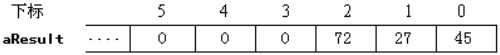
\includegraphics[width=260pt]{bigintmul1.png}\\
\end{center}

接下来算$4 \times 5$ 。此处$4 \times 5$的结果代表20个10 ,因此要 aResult[1]+=20,变为:
\begin{center}
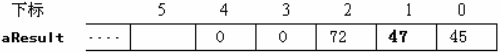
\includegraphics[width=260pt]{bigintmul2.png}\\
\end{center}

再下来算$4 \times 3$。此处$4 \times 3$的结果代表12个100,因此要 aResult[2]+= 12,变为:
\begin{center}
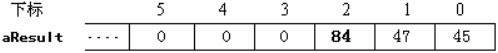
\includegraphics[width=260pt]{bigintmul3.png}\\
\end{center}

最后算$4 \times 8$。此处$4 \times 8$的结果代表32个1000 ,因此要 aResult[3]+= 32,变为:
\begin{center}
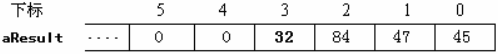
\includegraphics[width=260pt]{bigintmul4.png}\\
\end{center}

乘法过程完毕。接下来从 aResult[0] 开始向高位逐位处理进位问题。aResult[0]留下5,把4 加到aResult[1]上,aResult[1]变为 51 后,应留下 1 ,把5 加到aResult[2]上……最终使得aResult 里的每个元素都是 1 位数,结果就算出来了:
\begin{center}
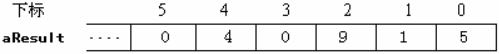
\includegraphics[width=260pt]{bigintmul5.png}\\
\end{center}

总结一个规律,即一个数的第i位和另一个数的第j位相乘所得的数,一定是要累加到结果的第i+j位上。这里i, j都是从右往左,从0开始数。

\subsubsection{代码}
\begin{Codex}[label=bigint_mul.c]
#include<stdio.h>
#include<string.h>

/* 一个数组元素表示4个十进制位,即数组是万进制的 */
#define BIGINT_MOD 10000
#define MOD_LEN 4
#define MAX_LEN (200/MOD_LEN+1)  /* 整数的最大位数 */

char    a[MAX_LEN * MOD_LEN], b[MAX_LEN * MOD_LEN];
int     x[MAX_LEN], y[MAX_LEN], z[MAX_LEN * 2];

/**
 * @brief 打印大整数.
 * @param[in] x 大整数,用数组表示,低位在低地址
 * @param[in] n 数组x的长度
 * @return 无
 */
void bigint_print(const int x[], const int n) {
    int i;
    int start_output = 0;  /* 用于跳过前导0 */
    for (i = n - 1; i >= 0; --i) {
        if (start_output) {  /* 如果多余的0已经都跳过,则输出 */
            printf("%04d", x[i]);
        } else if (x[i] > 0) {
            printf("%d", x[i]);
            start_output = 1; /* 碰到第一个非0的值,就说明多余的0已经都跳过 */
        }
    }

    if(!start_output) printf("0");  /* 当x全为0时 */
}

/**
 * @brief 将输入的字符串转化为大整数.
 * @param[in] s 输入的字符串
 * @param[out] x 大整数
 * @return 无
 */
void bigint_input(const char s[], int x[]) {
    int i, j = 0;
    const int len = strlen(s);
    for (i = 0; i < MAX_LEN; i++) x[i] = 0;

    // for (i = len - 1; i >= 0; i--) a[j++] = s[i] - '0';
    for (i = len; i > 0; i -= MOD_LEN) {  /* [i-MOD_LEN, i) */
        int temp = 0;
        int k;
        const int low = i-MOD_LEN > 0 ? i-MOD_LEN : 0;
        for (k = low; k < i; k++) {
            temp = temp * 10 + s[k] - '0';
        }

        x[j++] = temp;
    }
}

/**
 * @brief 大整数乘法.
 * @param[in] x x
 * @param[in] y y
 * @param[out] z z=x*y
 * @return 无
 */
void bigint_mul(const int x[], const int y[], int z[]) {
    int i, j;
    for (i = 0; i < MAX_LEN * 2; i++) z[i] = 0;

    for (i = 0; i < MAX_LEN; i++) {
        for (j = 0; j < MAX_LEN; j++) { /*用y[i],去乘以x的各位*/
            z[i + j] += y[i] * x[j];  /* 两数第i, j位相乘,累加到结果的第i+j位 */
        }
    }
    
    for (i = 0; i < MAX_LEN * 2; i++) {  /* 统一处理进位问题 */
        if (z[i] >= BIGINT_MOD) {  /* 看是否要进位 */
            z[i+1] += z[i] / BIGINT_MOD;  /* 进位 */
            z[i] %= BIGINT_MOD;
        }
    }
}


int main() {
    scanf("%s%s", a, b);

    bigint_input(a, x);
    bigint_input(b, y);

    bigint_mul(x, y, z);
    bigint_print(z, MAX_LEN * 2);
    printf("\n"); 
    return 0;
}
\end{Codex}

\subsubsection{类似的题目}
与本题相同的题目:
\begindot
\item 《程序设计导引及在线实践》\footnote{李文新,程序设计导引及在线实践, 清华大学出版社, 2007}第146页7.2节
\item 百练 2980 大整数乘法, \myurl{http://poj.grids.cn/practice/2980/}
\myenddot

与本题相似的题目:
\begindot
\item  TODO
\myenddot


\section{大整数除法} %%%%%%%%%%%%%%%%%%%%%%%%%%%%%%
\subsubsection{描述}
求两个非负的大整数相除的商。

\subsubsection{输入}
第1行是测试数据的组数T,每组测试数据占2行,第1行是被除数,第2行是除数,每行数据不超过100 个字符。每组测试数据之间有一个空行。

\subsubsection{输出}
每组测试数据输出一行,即相应的整数商

\subsubsection{样例输入}
\begin{Code}
3
2405337312963373359009260457742057439230496493930355595797660791082739646
2987192585318701752584429931160870372907079248971095012509790550883793197894

10000000000000000000000000000000000000000
10000000000

5409656775097850895687056798068970934546546575676768678435435345
1
\end{Code}

\subsubsection{样例输出}
\begin{Code}
0
1000000000000000000000000000000
5409656775097850895687056798068970934546546575676768678435435345
\end{Code}

\subsubsection{分析}
基本的思想是反复做减法,看看从被除数里最多能减去多少个除数,商就是多少。一个一个减显然太慢,如何减得更快一些呢?以 7546 除以23为例来看一下:开始商为0。先减去23的100倍,就是2300,发现够减3次,余下646。于是商的值就增加300。然后用646减去230,发现够减 2 次,余下 186,于是商的值增加20。最后用186减去23,够减8次,因此最终商就是328。

所以本题的核心是要写一个大整数的减法函数,然后反复调用该函数进行减法操作。

计算除数的10倍、100倍的时候,不用做乘法,直接在除数后面补0即可。

\subsubsection{代码}
\begin{Codex}[label=bigint_div.c]
#include <stdio.h>
#include <stdlib.h>
#include <string.h>

/* 一个数组元素表示4个十进制位,即数组是万进制的 */
#define BIGINT_MOD 10000
#define MOD_LEN 4
#define MAX_LEN (100/MOD_LEN+1)  /* 整数的最大位数 */

char    a[MAX_LEN * MOD_LEN], b[MAX_LEN * MOD_LEN];
int     x[MAX_LEN], y[MAX_LEN], z[MAX_LEN];

/**
 * @brief 打印大整数.
 * @param[in] x 大整数,用数组表示,低位在低地址
 * @param[in] n 数组x的长度
 * @return 无
 */
void bigint_print(const int x[], const int n) {
    int i;
    int start_output = 0;  /* 用于跳过前导0 */
    for (i = n - 1; i >= 0; --i) {
        if (start_output) {  /* 如果多余的0已经都跳过,则输出 */
            printf("%04d", x[i]);
        } else if (x[i] > 0) {
            printf("%d", x[i]);
            start_output = 1; /* 碰到第一个非0的值,就说明多余的0已经都跳过 */
        }
    }

    if(!start_output) printf("0");  /* 当x全为0时 */
}

/**
 * @brief 将输入的字符串转化为大整数.
 * @param[in] s 输入的字符串
 * @param[out] x 大整数
 * @return 无
 */
void bigint_input(const char s[], int x[]) {
    int i, j = 0;
    const int len = strlen(s);
    for (i = 0; i < MAX_LEN; i++) x[i] = 0;

    // for (i = len - 1; i >= 0; i--) a[j++] = s[i] - '0';
    for (i = len; i > 0; i -= MOD_LEN) {  /* [i-MOD_LEN, i) */
        int temp = 0;
        int k;
        const int low = i-MOD_LEN > 0 ? i-MOD_LEN : 0;
        for (k = low; k < i; k++) {
            temp = temp * 10 + s[k] - '0';
        }

        x[j++] = temp;
    }
}

/**
 * @brief 计算大整数的位数.
 *
 * @param[inout] x 大整数
 * @return 位数
 */
static int length(const int x[]) {
    int i;
    int result = 0;
    for (i = MAX_LEN - 1; i >= 0; i--) if (x[i] > 0) {
        result = i + 1;
        break;
    }
    return result;
}

/**
 * @brief 大整数减法.
 *
 * @param[inout] x x
 * @param[in] y y
 * @return 如果x < y,返回-1,如果x=y,返回0,如果x>y,返回1
 */
static int bigint_sub(int x[], const int y[]) {
    int i;
    const int lenx = length(x);
    const int leny = length(y);

    /* 判断x是否比y大 */
    if (lenx < leny) return -1;
    else if (lenx == leny) {
        int larger = 0;
        for (i = lenx - 1; i >= 0; i--) {
            if (x[i] > y[i]) {
                larger = 1;
            } else if (x[i] < y[i]) {
                if (!larger) return -1;
            }
        }
    }
    
    for (i = 0; i < MAX_LEN; i++) {  /* 逐位相减 */
        x[i] -= y[i];
        if (x[i] < 0) {  /* 看是否要借位 */
            x[i] += BIGINT_MOD;
            x[i+1] --;  /* 借位 */
        }
    }

    return 1;
}

/**
 * @brief 大整数除法.
 *
 * @param[inout] x x
 * @param[in] y y
 * @param[out] z z=x/y
 * @return 无
 */
void bigint_div(int x[], const int y[], int z[]) {
    int i;
    int *yy; /* y的副本 */
    const int xlen = length(x);
    int ylen = length(y);
    const int times = xlen - ylen;

    for (i = 0; i < MAX_LEN; i++) z[i] = 0;
    if (times < 0) return;

    yy = (int*)malloc(sizeof(int) * MAX_LEN);
    memcpy(yy, y, sizeof(int) * MAX_LEN);


    /* 将yy右移times位,使其长度和x相同,即 yy 乘以 10000 的times次幂 */
    for (i = xlen - 1; i >= 0; i--) {
        if (i >= times) yy[i] = yy[i - times];
        else yy[i] = 0;
    }

    /* 先减去若干个 y×(10000的 times次方), 
      不够减了,再减去若干个 y×(10000的 times-1次方)
      一直减到不够减为止 */
    ylen = xlen;
    for (i = 0; i <= times; i++) {
        int j;
        while (bigint_sub(x, yy) >= 0) {
            z[times - i]++;
        }

        /* yy 除以BIGINT_MOD,即左移一位 */
        for (j = 1; j < ylen; j++) {
            yy[j - 1] = yy[j];
        }
        yy[--ylen] = 0;
    }

    /* 下面的循环统一处理进位 */
    for (i = 0; i < MAX_LEN - 1; i++) {
        if (z[i] >= BIGINT_MOD) {  /* 看是否要进位 */
            z[i+1] += z[i] / BIGINT_MOD;  /* 进位 */
            z[i] %= BIGINT_MOD;
        }
    }
    free(yy);
}

int main() {
    int T;    
    scanf("%d", &T);

    while (T-- > 0) {
        scanf("%s%s",a,b);

        bigint_input(a, x);
        bigint_input(b, y);

        bigint_div(x, y, z);
        bigint_print(z, MAX_LEN);
        printf("\n"); 
    }
    return 0;
}
\end{Codex}

\subsubsection{类似的题目}
与本题相同的题目:
\begindot
\item 《程序设计导引及在线实践》\footnote{李文新,程序设计导引及在线实践, 清华大学出版社, 2007}第149页7.3节
\item 百练 2737 大整数除法, \myurl{http://poj.grids.cn/practice/2737/}
\myenddot

与本题相似的题目:
\begindot
\item  TODO
\myenddot

\chapter{基础功能}
在面试和笔试中,经常会出现这类题目,把C++, Java标准库中的一些函数单独拿出来,让你重新实现。这类题目短小精悍,很能考验一个人的基本功是否扎实。

\section{下一个排列} %%%%%%%%%%%%%%%%%%%%%%%%%%%%%%
\label{sec:nextpermutation}

\subsubsection{描述}
实现C++ STL 中的 \fn{next_permutation()},函数原型如下:

\begin{Code}
/**
 * @brief 返回下一个排列,例如当前排列是12345,下一个是12354
 * @param[inout] num 当前排列,例如 12345
 * @param[in] len num的长度
 * @return 无
 */
void next_permutation(int num[], int len);
\end{Code}

\subsubsection{分析}
算法过程如图~\ref{fig:permutation}所示(来自\myurl{http://fisherlei.blogspot.com/2012/12/leetcode-next-permutation.html})。

\begin{center}
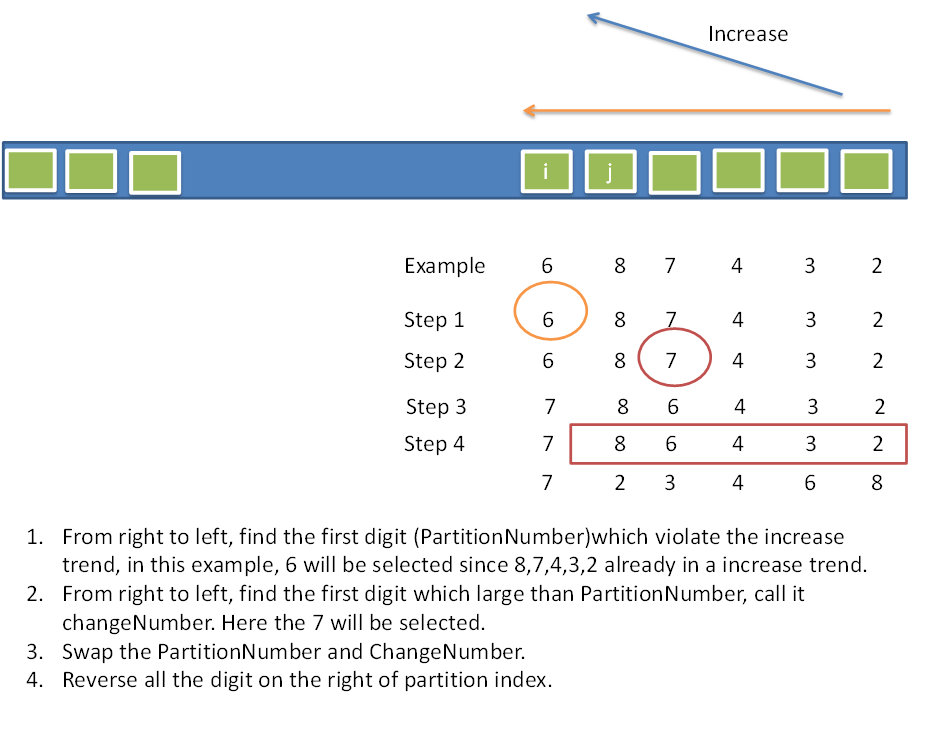
\includegraphics[width=360pt]{next-permutation.png}\\
\figcaption{下一个排列算法流程}\label{fig:permutation}
\end{center}

\subsubsection{代码}

\begin{Codex}[label=next_permutation.c]
static void swap(int array[], int i, int j) {
    const int tmp = array[i];
    array[i] = array[j];
    array[j] = tmp;
}

static void reverse(int array[], int first, int last) { //左闭右开区间
    last--;
    while (first < last)
        swap(array, first++, last--);
}

/**
 * @brief 返回下一个排列,例如当前排列是12345,下一个是12354
 * @param[inout] num 当前排列,例如 12345
 * @param[in] first 开始位置
 * @param[in] last 结束位置,左闭右开区间
 * @return 成功返回 0,失败返回 -1
 */
int next_permutation(int num[], int first, int last) {
    int i, j;

    i = last - 2;  // partition number's index
    while (i >= 0 && num[i] >= num[i + 1])
        i--;

    if (i == -1) {
        reverse(num, first, last);
        return -1;
    }

    j = last - 1;  // change number's index
    while (num[j] <= num[i])
        --j;
    swap(num, i, j);
    reverse(num, i + 1, last);

    return 0;
}
\end{Codex}

\subsubsection{相关的题目}
与本题相同的题目:
\begindot
\item LeetCode -  Next Permutation, \myurl{http://leetcode.com/onlinejudge\#question_31}
\myenddot


\section{数组循环右移} %%%%%%%%%%%%%%%%%%%%%%%%%%%%%%

\subsubsection{描述}
将一个长度为n的数组A的元素循环右移(ROR, Rotate Right)k位,比如数组 {1, 2, 3, 4, 5}循环右移3位之后就变成{3, 4, 5, 1, 2}。

\subsubsection{方法一}
最直接的做法是另开一个大小一样的数组B,遍历一下,令$B[(i + k) \% n] = A[i]$,再将B的内容写回到A即可。这个方法的时间复杂度为O(n),空间复杂度也为O(n)。代码如下:

\begin{Codex}[label=ror.c]
void ror1(int array[], int n, int k) {
    int i;
    int *B = (int*) malloc(n * sizeof(int));

    k %= n;
    if (k == 0)
        return;

    for (i = 0; i < n; i++) {
        B[(i + k) % n] = array[i];
    }
    for (i = 0; i < n; i++) {
        array[i] = B[i];
    }
}
\end{Codex}

\subsubsection{方法二}
另一种简单的做法,每次将数组中的所有元素右移一位,循环k次。这个方法的时间复杂度为O(n*k),空间复杂度为O(1)。代码如下:

\begin{Codex}[label=ror.c]
void ror2(int array[], int n, int k) {
    int i, tmp;
    k %= n;
    if (k == 0)
        return;

    while (k--) {
        tmp = array[n - 1];
        for (i = n - 1; i > 0; i--) {
            array[i] = array[i - 1];
        }
        array[0] = tmp;
    }
}
\end{Codex}

\subsubsection{方法三}
先将A的元素倒置,即{1, 2, 3, 4, 5}变成{5, 4, 3, 2, 1},然后将前k位倒置,即{3, 4, 5, 2, 1},再将后n-k位倒置,即{3, 4, 5, 1, 2},完成。

证明:记A的前n-k位为X,后k位为Y,则A=XY,将A循环右移k位后,应该得到YX。根据该算法,先将A整体倒置,得到$(XY)^T=Y^TX^T$,然后将前k位倒置,得到$YX^T$,最后将后n-k位倒置,得到YX,正好是所求的结果,证毕。

这个方法的时间复杂度为O(2n),空间复杂度为O(1)。代码如下:

\begin{Codex}[label=ror.c]
static void swap(int array[], int i, int j) {
    const int temp = array[i];
    array[i] = array[j];
    array[j] = temp;
}

static void reverse(int array[], int begin, int end) { //左闭右开区间
    end--;
    while (begin < end)
        swap(array, begin++, end--);
}

void ror3(int *array, int n, int k) {
    k %= n;
    if (k == 0)
        return;

    reverse(array, 0, n);
    reverse(array, 0, k);
    reverse(array, k, n - k);
}
\end{Codex}

这种方法需要对每个位置写入2次,看上去也不怎么好,那有没有更好的呢?

\subsubsection{方法四}
我们要做的只是把每个元素放到它应该在的位置,比如开头的例子,1应该放在4的位置,把1放好之后,4就没地方了,那4应该在哪呢,在2的位置,依此类推,就可以把所有的元素都放好,而且只放了一次。看上去这样做很完美,但仔细想想就能想出反例子,比如{1, 2, 3, 4, 5, 6, 7, 8, 9}右移3位,就是1放在4个位置,4放在7的位置,然后7放回1,这时候一圈兜完了,但只排好了3个元素,剩下的6个元素没有动过,怎么办呢?继续下一个,就是2,然后2、5、8也排好了,继续3、6、9,这时候下一个元素是1了,应该停止了(因为1、4、7已经排好了),那程序怎么会知道停在这里了,于是就想到了最大公约数,9和3的最大公约数是3,于是做前3个数的循环就可以了,为什么上一个例子只需做一次,因为元素个数(5)和移动位数(3)互质。具体的数学证明略。

代码如下:

\begin{Codex}[label=ror.c]
static int gcd(int a, int b) {
    assert(a >= b);
    if (b == 0) {
        return a;
    }

    while (b > 0) {
        int tmp = a % b;
        a = b;
        b = tmp;
    }

    return a;
}

void ror4(int *array, int n, int k) {
    int i;
    const int g = gcd(n, k);

    k %= n;
    if (k == 0)
        return;

    for (i = 0; i < g; ++i) {
        int j = i;
        int cur = array[j], tmp;

        do {
            tmp = array[(j + k) % n];
            array[(j + k) % n] = cur;
            cur = tmp;
            j = (j + k) % n;
        } while (j != i);
    }
}

// test
int main(void) {
    int i;
    int a[] = { 1, 2, 3, 4, 5 };
    ror4(a, 5, 3);
    for (i = 0; i < 5; i++) {
        printf("%d ", a[i]);
    }

    return EXIT_SUCCESS;
}
\end{Codex}


\appendix % 开始附录,章用字母编号
\printindex

\end{document}
